% ===== Document Class & Packages =====
\documentclass[12pt,hidelinks]{book}
    \usepackage{url}
    \usepackage{acronym}
    \usepackage{adjustbox}
    \usepackage[backend=bibtex, sorting=none, defernumbers=true]{biblatex}
    \addbibresource{./Chapters/Bibliography/c++.bib}
    \addbibresource{./Chapters/Bibliography/idioms.bib}
    \addbibresource{./Chapters/Bibliography/memorymanagement.bib}
    \addbibresource{./Chapters/Bibliography/smartpointers.bib}
    \addbibresource{./Chapters/Bibliography/containers.bib}
    \addbibresource{./Chapters/Bibliography/concurrency.bib}
    \addbibresource{./Chapters/Bibliography/linuxprocesses.bib}
    \addbibresource{./Chapters/Bibliography/memorymodel.bib}
    \addbibresource{./Chapters/Bibliography/cacheperformance.bib}
    \addbibresource{./Chapters/Bibliography/numa.bib}
    \addbibresource{./Chapters/Bibliography/linuxnetworking.bib}
    \addbibresource{./Chapters/Bibliography/eventdrivenio.bib}
    \addbibresource{./Chapters/Bibliography/memorymapping.bib}
    \addbibresource{./Chapters/Bibliography/kernelbypass.bib}
    \addbibresource{./Chapters/Bibliography/lowlatency.bib}
    \addbibresource{./Chapters/Bibliography/algorithms.bib}
    \addbibresource{./Chapters/Bibliography/designpatterns.bib}
    \addbibresource{./Chapters/Bibliography/solidprinciples.bib}
    \addbibresource{./Chapters/Bibliography/umlandoop.bib}
    \addbibresource{./Chapters/Bibliography/python.bib}
    \addbibresource{./Chapters/Bibliography/testing.bib}
    \addbibresource{./Chapters/Bibliography/ai.bib}
    \addbibresource{./Chapters/Bibliography/dictionary.bib}
    % Shared bibliography helpers. .bib files are the single source of truth.
\newcommand{\printbibsection}[3]{%
    \printbibliography[heading=#1,keyword={#2},title={#3}]%
}


    \usepackage{layouts}
    \usepackage{layout}
    \usepackage{tocbibind}
	\usepackage{lipsum} 
	\usepackage[explicit]{titlesec}
	\usepackage{titletoc}
	\usepackage{tocloft}
	\usepackage{charter}
	\usepackage[many]{tcolorbox}
	\usepackage{amssymb,amsmath,amsthm}
    \newtheorem{theorem}{Theorem}
    \newtheorem{definition}{Definition}
    \usepackage{mathtools} % Bonus
    \usepackage{subcaption}
	\usepackage{graphicx}
	\usepackage{wrapfig}
    \usepackage{todonotes}
    \usepackage{float}
    \usepackage{subcaption}
    \usepackage{colortbl}
	\usepackage{xcolor}
	\usepackage{tikz,lipsum,lmodern}
    \usetikzlibrary{arrows,arrows.meta}
    \usepackage{pgf-umlcd}
    \renewcommand{\umldrawcolor}{black}
    \renewcommand{\umlfillcolor}{white}
    \usetikzlibrary{positioning}
    \usetikzlibrary{shapes.geometric,shapes.multipart}
    \usetikzlibrary{decorations.text}
	\usetikzlibrary{calc}
	\usepackage[english]{babel}
	\usepackage{fancyhdr}
	\usepackage{mathrsfs}
	\usepackage{empheq}
	\usepackage{fourier}% change to lmodern if fourier is no available
	\usepackage{wrapfig}
	\usepackage{fancyref}
	\usepackage{hyperref}
	\usepackage{cleveref}
	\usepackage{listings}
	\usepackage{varwidth}
	\usepackage{longfbox}
	\usepackage{geometry}
	\usepackage{marginnote}
    \usepackage{multicol, multirow}
    \usepackage{tabularx}
    \usepackage{caption}
	\tcbuselibrary{theorems}
	\tcbuselibrary{breakable, skins}
	\tcbuselibrary{listings, documentation}
	\geometry{
		a4paper,
		left=33mm,
		right=33mm,
		top=20mm}
    \usepackage{ifthen}
    
% ========= Path to images ============
%   - Direct the computer on the path 
% 	  to the folder containg the images
% =====================================
\graphicspath{{./images/}}

% ========= Caption Setup =============
\DeclareCaptionFormat{custom}
{
    \textbf{#1#2}\textit{\small #3}
}
\captionsetup{format=custom}

% ============= Macros ================
\newcommand{\fillin}{\underline{\hspace{.75in}}{\;}}
\newcommand{\solution}{\textcolor{mordantred19}{Solution:}}
\setlength{\parindent}{0pt}
\addto{\captionsenglish}{\renewcommand*{\contentsname}{Table of Contents}}
\linespread{1.2}

% ======= Sections redefinitions ======
\newcommand{\nparagraph}[1]{\paragraph{#1}\mbox{}\\}
\newcommand{\toclessnparagraph}[1]{\paragraph*{#1}\mbox{}\\}
\newcommand{\nsubparagraph}[1]{\subparagraph{#1}\mbox{}\\}
\newcommand{\toclessnsubparagraph}[1]{\subparagraph*{#1}\mbox{}\\}

% ======== Dictionary Entries =========
% Defines the command to print each word on the page,
% \markboth{}{} prints the first word on the page in the top left header and the last word in the top right
\newcommand{\dictentry}[2]{\markboth{#1}{#1}\textbf{#1} \ $\bullet$\ {#2}}  

% ======== Class Diagrams ====
\newcommand{\operationtt}[1]{\operation{\footnotesize{\texttt{#1}}}}
\newcommand{\attributett}[1]{\attribute{\footnotesize{\texttt{#1}}}}

% ========== Defined Commands =========
\def\CC{{C\nolinebreak[4]\hspace{-.05em}\raisebox{.4ex}{\tiny\bf ++}}}

% ======== Fancy Pagestyles ===========
\fancypagestyle{basicstyle}{
    \renewcommand{\headrulewidth}{0pt}
    \fancyhead{}
    \fancyfoot{}
    \fancyfoot[C]{\textbf{\thepage}}}

\fancypagestyle{dictionarystyle}{
    \renewcommand{\headrulewidth}{0.4pt}
    \pagestyle{fancy}
    \fancyhead{}
    \fancyfoot{}
    \fancyfoot[C]{\textbf{\thepage}}
    \fancyhead[LE,LO]{\textbf{\rightmark}}
    \fancyhead[RE,RO]{\textbf{\leftmark}}
    }
    
% =====================================
\renewcommand{\thechapter}{\arabic{chapter}}
\renewcommand{\thesection}{\thechapter.\arabic{section}}
\renewcommand{\thesubsection}{\thesection.\arabic{subsection}}
\newcommand\sectionnumfont{% font specification for the number
	\fontsize{380}{130}\color{myblueii}\selectfont}
\newcommand\sectionnamefont{% font specification for the name "PART"
	\normalfont\color{white}\scshape\small\bfseries }
    
% ============= Colors ================
% ----- Red
\definecolor{mordantred19}{rgb}{0.68, 0.05, 0.0}
% ----- Blue
\definecolor{st.patrick\'sblue}{rgb}{0.14, 0.16, 0.48}
\definecolor{teal}{rgb}{0.0, 0.5, 0.5}
\definecolor{beaublue}{rgb}{0.74, 0.83, 0.9}
\definecolor{mybluei}{RGB}{0,173,239}
\definecolor{myblueii}{RGB}{63,200,244}
\definecolor{myblueiii}{RGB}{199,234,253}
% ----- Yellow
\definecolor{blond}{rgb}{0.98, 0.94, 0.75}
\definecolor{cream}{rgb}{1.0, 0.99, 0.82}
% ----- Green
\definecolor{emerald}{rgb}{0.31, 0.78, 0.47}
\definecolor{darkspringgreen}{rgb}{0.09, 0.45, 0.27}
% ----- White
\definecolor{ghostwhite}{rgb}{0.97, 0.97, 1.0}
\definecolor{splashedwhite}{rgb}{1.0, 0.99, 1.0}
% ----- Grey
\definecolor{whitesmoke}{rgb}{0.96, 0.96, 0.96}
\definecolor{lightgray}{rgb}{0.92, 0.92, 0.92}
\definecolor{floralwhite}{rgb}{1.0, 0.98, 0.94}

% ----- Colors added by me
% Oblivion 2 (Geany) token colors — listing background stays light
\definecolor{obliviondefault}{HTML}{2E3436}
\definecolor{oblivionkeyword}{HTML}{4E9A06}
\definecolor{obliviontype}{HTML}{3465A4}
\definecolor{oblivionstring}{HTML}{C4A000}
\definecolor{oblivioncomment}{HTML}{888A85}
\definecolor{oblivionnumber}{HTML}{CC0000}
\definecolor{oblivionpreproc}{HTML}{75507B}
\definecolor{oblivionnamespace}{HTML}{75507B}
\definecolor{codegreen}{HTML}{888A85}
\definecolor{codegray}{HTML}{888A85}
\definecolor{codepurple}{HTML}{C4A000}
\definecolor{backcolour}{rgb}{0.95,0.95,0.92}

\definecolor{shadecolor}{RGB}{0,140,69}      
\definecolor{textcolor}{RGB}{0, 61, 165}  

% ========== Text Highlight ===========
\definecolor{tpgray}{gray}{0.90}
\newtcbox\tcbtp{hbox, on line, colback=tpgray, enhanced, frame hidden, boxrule=0pt, 
    top=-2pt, bottom=-2pt, right=-2pt, left=-2pt, rounded corners}
\newcommand{\highlight}[2][textcolor]{\tcbtp{{\color{#1}{#2}}}}
\newcommand{\highlightit}[2][textcolor]{\tcbtp{\textit{\color{#1}{#2}}}}
\newcommand{\highlighttt}[2][textcolor]{\tcbtp{\texttt{\color{#1}{#2}}}}
\newcommand{\highlightbf}[2][textcolor]{\tcbtp{\textbf{\color{#1}{#2}}}}
\newcommand{\inlinecode}[1]{\tcbtp{\texttt{\color{textcolor}{#1}}}}


% ======= Part Title Format ========
\titleformat{\part}[display]
{\normalfont\huge\filleft}
{}
{20pt}
{\begin{tikzpicture}[remember picture,overlay]
    \fill[myblueiii]
    (current page.north west) rectangle ([yshift=-13cm]current page.north east);
\node[
    fill=mybluei,
    text width=2\paperwidth,
    rounded corners=6cm,
    text depth=18cm,
    anchor=center,
    inner sep=0pt] at (current page.north east) (partbanner) {};
\node[
    anchor=south east,
    inner sep=0pt,
    outer sep=0pt] (partnum) at ([xshift=-20pt]partbanner.south)
    {\sectionnumfont\thepart};
\node[
    anchor=south,
    inner sep=0pt] (partname) at ([yshift=2pt]partnum.south)
    {\sectionnamefont PART};
\node[
    anchor=north east,
    align=right,
    inner xsep=0pt] at ([yshift=-0.5cm]partname.east|-partnum.south)
    {\parbox{.7\textwidth}{\raggedleft#1}};
\end{tikzpicture}%
}

% ======= Chapter Title Format ========
\titleformat{\chapter}
{\normalfont\huge\filleft}
{}
{20pt}
{\begin{tikzpicture}[remember picture,overlay]
    \fill[myblueiii] 
    (current page.north west) rectangle ([yshift=-13cm]current page.north east);   
\node[
    fill=mybluei,
    text width=2\paperwidth,
    rounded corners=6cm,
    text depth=18cm,
    anchor=center,
    inner sep=0pt] at (current page.north east) (parttop)
    {\thepart};%
\node[
    anchor=south east,
    inner sep=0pt,
    outer sep=0pt] (partnum) at ([xshift=-20pt]parttop.south) 
    {\sectionnumfont\thechapter}; % changed \thesection to \thechapter
\node[
    anchor=south,
    inner sep=0pt] (partname) at ([yshift=2pt]partnum.south)   
    {\sectionnamefont CHAPTER}; % chandeg SECTION to CHAPTER
\node[
    anchor=north east,
    align=right,
    inner xsep=0pt] at ([yshift=-0.5cm]partname.east|-partnum.south) 
    {\parbox{.7\textwidth}{\raggedleft#1}};
\end{tikzpicture}%
}

% Chapter titles use a TikZ overlay banner; push body text below it globally.
\titlespacing*{\chapter}{0pt}{0pt}{10.5cm}


% ============= Hyper Ref =============
\hypersetup{
	colorlinks,
	linkcolor={red!50!black},
	citecolor={blue!50!black},
	urlcolor={blue!80!black}
}

% ====== lstlisting environment =======
% Token colors inspired by Geany "Oblivion 2" (on light listing background).
% Built-in language keywords -> green. Custom types/namespaces use emph (morekeywords
% inside a style are cleared when language=C++/Python is set on a listing).
\lstdefinestyle{mystyle}{
    backgroundcolor=\color{backcolour},
    basicstyle=\ttfamily\footnotesize\color{obliviondefault},
    keywordstyle={\color{oblivionkeyword}\bfseries},
    commentstyle={\color{oblivioncomment}\itshape},
    stringstyle={\color{oblivionstring}},
    numberstyle=\tiny\color{codegray},
    alsoletter={_},
    % Types / typedefs (add new names here as examples need them)
    emph={bool,char,short,int,long,float,double,void,unsigned,signed,const,volatile,auto,
          size_t,ssize_t,pid_t,uint8_t,uint16_t,uint32_t,uint64_t,
          int8_t,int16_t,int32_t,int64_t,char8_t,char16_t,char32_t,byte,nullptr_t,
          string,string_view,wstring_view,thread,jthread,vector,array,map,unordered_map,span,optional,variant,any,
          mutex,atomic,atomic_flag,unique_ptr,shared_ptr,weak_ptr,lock_guard,unique_lock,
          condition_variable,future,promise,pair,initializer_list,
          cpu_set_t,sched_param,pthread_t,sockaddr,sockaddr_in,enable_if_t,remove_reference_t,is_same_v,integer_sequence,
          steady_clock,system_clock,high_resolution_clock,time_point,duration,complex,path,iostream,
          True,False,None,str,list,dict,set,tuple,bytes},
    emphstyle={\color{obliviontype}\bfseries},
    % Namespaces (std::thread -> std purple, thread blue above)
    emph={[2]std,this_thread,chrono,filesystem},
    emphstyle={[2]\color{oblivionnamespace}\bfseries},
    % Methods / free functions you care to highlight in examples
    emph={[3]get_id,native_handle,getpid,pthread_self,syscall,make_unique,make_shared},
    emphstyle={[3]\color{obliviontype}},
    breakatwhitespace=false,
    breaklines=true,
    captionpos=b,
    keepspaces=true,
    numbers=left,
    numbersep=8pt,
    numberfirstline=true,
    frame=single,
    framerule=0.4pt,
    rulecolor=\color{codegray},
    framesep=4pt,
    xleftmargin=1.6em,
    xrightmargin=0.4em,
    aboveskip=\medskipamount,
    belowskip=\medskipamount,
    showspaces=false,
    showstringspaces=false,
    showtabs=false,
    tabsize=2
}

\lstdefinelanguage{C+++}{%
  language     = C++,
  otherkeywords = {::, *, &, &&},
}

\lstset{style=mystyle}

% Re-apply emph after each language=... switch (listings drops style morekeywords).
\makeatletter
\lst@AddToHook{SetLanguage}{%
  \lstset{%
    alsoletter={_},%
    emph={bool,char,short,int,long,float,double,void,unsigned,signed,const,volatile,auto,
          size_t,ssize_t,pid_t,uint8_t,uint16_t,uint32_t,uint64_t,
          int8_t,int16_t,int32_t,int64_t,char8_t,char16_t,char32_t,byte,nullptr_t,
          string,string_view,wstring_view,thread,jthread,vector,array,map,unordered_map,span,optional,variant,any,
          mutex,atomic,atomic_flag,unique_ptr,shared_ptr,weak_ptr,lock_guard,unique_lock,
          condition_variable,future,promise,pair,initializer_list,
          cpu_set_t,sched_param,pthread_t,sockaddr,sockaddr_in,enable_if_t,remove_reference_t,is_same_v,integer_sequence,
          steady_clock,system_clock,high_resolution_clock,time_point,duration,complex,path,iostream,
          True,False,None,str,list,dict,set,tuple,bytes},%
    emphstyle={\color{obliviontype}\bfseries},%
    emph={[2]std,this_thread,chrono,filesystem},%
    emphstyle={[2]\color{oblivionnamespace}\bfseries},%
    emph={[3]get_id,native_handle,getpid,pthread_self,syscall,make_unique,make_shared},%
    emphstyle={[3]\color{obliviontype}},%
  }%
}
\makeatother

% ========= Example Boxes =============
\tcbset{
	defstyle/.style={
		fonttitle=\bfseries\upshape, 
		fontupper=\slshape,
		arc=0mm, 
		beamer,
		colback=blue!5!white,
		colframe=blue!75!black},
	theostyle/.style={
		fonttitle=\bfseries\upshape, 
		fontupper=\slshape,
		colback=red!10!white,
		colframe=red!75!black},
	visualstyle/.style={
		height=6.5cm,
		breakable,
		enhanced,
		leftrule=0pt,
		rightrule=0pt,
		bottomrule=0pt,
		outer arc=0pt,
		arc=0pt,
		colframe=mordantred19,
		colback=lightgray,
		attach boxed title to top left,
		boxed title style={
			colback=mordantred19,
			outer arc=0pt,
			arc=0pt,
			top=3pt,
			bottom=3pt,
		},
		fonttitle=\sffamily,},
	discussionstyle/.style={
		height=6.5cm,
		breakable,
		enhanced,
		rightrule=0pt,
		toprule=0pt,
		outer arc=0pt,
		arc=0pt,
		colframe=mordantred19,
		colback=lightgray,
		attach boxed title to top left,
		boxed title style={
			colback=mordantred19,
			outer arc=0pt,
			arc=0pt,
			top=3pt,
			bottom=3pt,
		},
		fonttitle=\sffamily},
	mystyle/.style={
		height=6.5cm,
		breakable,
		enhanced,
		rightrule=0pt,
		leftrule=0pt,
		bottomrule=0pt,
		outer arc=0pt,
		arc=0pt,
		colframe=mordantred19,
		colback=lightgray,
		attach boxed title to top left,
		boxed title style={
			colback=mordantred19,
			outer arc=0pt,
			arc=0pt,
			top=3pt,
			bottom=3pt,
		},
		fonttitle=\sffamily},
	aastyle/.style={
			height=3.5cm,
			enhanced,
			colframe=teal,
			colback=lightgray,
			colbacktitle=floralwhite,
			fonttitle=\bfseries,
			coltitle=black,
		attach boxed title to top center={
	  		yshift=-0.25mm-\tcboxedtitleheight/2,
	   		yshifttext=2mm-\tcboxedtitleheight/2}, 
		boxed title style={boxrule=0.5mm,
			frame code={ \path[tcb fill frame] ([xshift=-4mm]frame.west)
				-- (frame.north west) -- (frame.north east) -- ([xshift=4mm]frame.east)
				-- (frame.south east) -- (frame.south west) -- cycle; },
			interior code={ 
				\path[tcb fill interior] ([xshift=-2mm]interior.west)
				-- (interior.north west) -- (interior.north east)
				-- ([xshift=2mm]interior.east) -- (interior.south east) -- (interior.south west)
				-- cycle;} }
				},
	examstyle/.style={
		height=9.5cm,
		breakable,
		enhanced,
		rightrule=0pt,
		leftrule=0pt,
		bottomrule=0pt,
		outer arc=0pt,
		arc=0pt,
		colframe=mordantred19,
		colback=lightgray,
		attach boxed title to top left,
		boxed title style={
			colback=mordantred19,
			outer arc=0pt,
			arc=0pt,
			top=3pt,
			bottom=3pt,
		},
		fonttitle=\sffamily},
	doc head command={
		interior style={
			fill,
			left color=yellow!20!white, 
			right color=white}},
	doc head environment={
		boxsep=4pt,
		arc=2pt,
		colback=yellow!30!white,
		},
	doclang/environment content=text
}
% ============= Boxes ================
\newtcolorbox[auto counter,number within=section]{example}[1][]{
	mystyle,
	title=Example~\thetcbcounter,
	overlay unbroken and first={
		\path
		let
		\p1=(title.north east),
		\p2=(frame.north east)
		in
		node[anchor=
			west,
			font=\sffamily,
			color=st.patrick\'sblue,
			text width=\x2-\x1] 
		at (title.east) {#1};
	}
}
\newtcolorbox[auto counter,number within=section]{longexample}[1][]{
	examstyle,
	title=Example~\thetcbcounter,
	overlay unbroken and first={
		\path
		let
		\p1=(title.north east),
		\p2=(frame.north east)
		in
		node[anchor=
		west,
		font=\sffamily,
		color=st.patrick\'sblue,
		text width=\x2-\x1] 
		at (title.east) {#1};
	}
}
\newtcolorbox[auto counter,number within=section]{example2}[1][]{
	aastyle,
	title=Example~\thetcbcounter,{}
}
\newtcolorbox[auto counter,number within=section]{discussion}[1][]{
	discussionstyle,
	title=Discussion~\thetcbcounter,
	overlay unbroken and first={
		\path
		let
		\p1=(title.north east),
		\p2=(frame.north east)
		in
		node[anchor=
		west,
		font=\sffamily,
		color=st.patrick\'sblue,
		text width=\x2-\x1] 
		at (title.east) {#1};
	}
}
\newtcolorbox[auto counter,number within=section]{visualization}[1][]{
	visualstyle,
	title=Visualization~\thetcbcounter,
	overlay unbroken and first={
		\path
		let
		\p1=(title.north east),
		\p2=(frame.north east)
		in
		node[anchor=
		west,
		font=\sffamily,
		color=st.patrick\'sblue,
		text width=\x2-\x1] 
		at (title.east) {#1};
	}
}
% --------- Theorems ---------
\newtcbtheorem[number within=subsection,crefname={definition}{definitions}]%
	{Definition}{Definition}{defstyle}{def}%
\newtcbtheorem[use counter from=Definition,crefname={theorem}{theorems}]%
	{Theorem}{Theorem}{theostyle}{theo}
	%
\newtcbtheorem[use counter from=Definition]{theo}{Theorem}%
{
	theorem style=plain,
	enhanced,
	colframe=blue!50!black,
	colback=yellow!20!white,
	coltitle=red!50!black,
	fonttitle=\upshape\bfseries,
	fontupper=\itshape,
	drop fuzzy shadow=blue!50!black!50!white,
	boxrule=0.4pt}{theo}
\newtcbtheorem[use counter from=Definition]{DashedDefinition}{Definition}%
 {
 	enhanced,
 	frame empty,
 	interior empty,
 	colframe=darkspringgreen!50!white,
	coltitle=darkspringgreen!50!black,
	fonttitle=\bfseries,
	fonttitle=\bfseries,colbacktitle=darkspringgreen!15!white,
	borderline={0.5mm}{0mm}{darkspringgreen!15!white},
	borderline={0.5mm}{0mm}{darkspringgreen!50!white,dashed},
	attach boxed title to top center={yshift=-2mm},
	boxed title style={boxrule=0.4pt},
	varwidth boxed title}{theo}
%%%%%%%%%%%%%%%%%%%%%%%%%%%%%%%%%%%%%%%%
\newtcblisting[auto counter,number within=section]{disexam}{
	skin=bicolor,
	colback=white!30!beaublue,
	colbacklower=white,
	colframe=black,
	before skip=\medskipamount,
	after skip=\medskipamount,
	fontlower=\footnotesize,
	listing options={style=tcblatex,texcsstyle=*\color{red!70!black}},}
%%%%%%%%%%%%%%%%%%%%%%%%%%%%%%%%%%%%%%%

\pagestyle{basicstyle}
\begin{document}
\begin{titlepage}
	\centering % Center everything on the title page
	\scshape % Use small caps for all text on the title page
	\vspace*{1.5\baselineskip} % White space at the top of the page
    
% ===================
%	Title Section 	
% ===================

	\rule{13cm}{1.6pt}\vspace*{-\baselineskip}\vspace*{2pt} % Thick horizontal rule
	\rule{13cm}{0.4pt} % Thin horizontal rule
	
		\vspace{0.75\baselineskip} % Whitespace above the title
% ========== Title ===============	
	{	\Huge Software Engineering\\ 
			\vspace{4mm}
		Notebook \\	}
% ======================================
		\vspace{0.75\baselineskip} % Whitespace below the title
	\rule{13cm}{0.4pt}\vspace*{-\baselineskip}\vspace{3.2pt} % Thin horizontal rule
	\rule{13cm}{1.6pt} % Thick horizontal rule
	
		\vspace{1.75\baselineskip}
\end{titlepage}
\tableofcontents

\newpage
\newgeometry{
	left=29mm, 
	right=29mm, 
	top=20mm, 
	bottom=15mm}
\nocite{*}
\part{C++ Foundations}
\section{C++}
\label{sec:c++newfeatures}
\vspace{10.5cm}
\subsection{C++ Good Practices}
\subsubsection{Rule of three/five/zero}
\nparagraph{Rule of three}
If a class requires a \textbf{user-defined destructor}, a user-defined 
\textbf{copy constructor}, or a user-defined \textbf{copy assignment 
operator}, it almost certainly requires all three.

Because C++ copies and copy-assigns objects of user-defined types in 
various situations (passing/returning by value, manipulating a 
container, etc), these special member functions will be called, 
if accessible, and if they are not user-defined, they are 
implicitly-defined by the compiler.

The implicitly-defined special member functions are typically incorrect 
if the class manages a resource whose handle is an object of non-class 
type (raw pointer, POSIX file descriptor, etc), whose destructor does 
nothing and copy constructor/assignment operator performs a 
"shallow copy" (copy the value of the handle, without duplicating the 
underlying resource).

%~ \textbf{CODE EXAMPLE HERE}

Classes that manage non-copyable resources through copyable handles 
may have to declare copy assignment and copy constructor private 
and not provide their definitions or define them as deleted. 
This is another application of the rule of three: deleting one 
and leaving the other to be implicitly-defined will most likely result 
in errors.

\nparagraph{Rule of five}
Because the presence of a user-defined destructor, copy-constructor, 
or copy-assignment operator prevents the implicit definition of the 
move constructor and the move assignment operator, \textbf{any class 
for which move semantics are desirable}, has to declare all five special 
member functions.

%~ \textbf{CODE EXAMPLE HERE}

Unlike Rule of Three, 
failing to provide move constructor and move assignment 
is usually not an error, 
but a missed optimization opportunity.

\nparagraph{Rule of zero}
Classes that have custom 
destructors, copy/move constructors or copy/move assignment operators 
should deal exclusively with ownership 
(which follows from the Single Responsibility Principle). 
Other classes should not have custom 
destructors, copy/move constructors or copy/move assignment operators.
(see~\cite{fernandesruleofzero})

This rule also appears 
in the C++ Core Guidelines as C.20: 
If you can avoid defining default operations, do.

When a \textbf{base class is intended for polymorphic use}, 
its destructor may have to be declared public and virtual. 
This blocks implicit moves (and deprecates implicit copies), 
and so the special member functions have to be declared as defaulted
(see~\cite{meyersconcernaboutruleof0})

However, this makes the class prone to slicing, 
which is why polymorphic classes often 
define copy as deleted 
(see~\cite{cpp-core-guidelines-C67}), 
which leads to the following generic wording for the Rule of Five:
If you define or =delete any default operation, 
define or =delete them all
(see~\cite{cpp-core-guidelines-C21})

\subsubsection{Const Correctness}
Const Correctness consists in using the keyword \texttt{const} to 
prevent \texttt{const} objects from being mutated.

\nparagraph{const and pointer combinations}
Reading it right-to-left
\begin{table}[h!t]
    \begin{tabular}{l|r}
        \texttt{const X* p} & p is a pointer to an X that is constant.\\
        \hline
        \texttt{X const* p} & equivalent to \texttt{const X* p}.\\
        \hline
        \texttt{X* const p} & p is a \texttt{const} pointer to an X that 
                              is not \texttt{const}.\\
        \hline
        \texttt{const X* const p} &  p is a \texttt{const} pointer to an 
                                     X that is \texttt{const}.\\
    \end{tabular}
\end{table}

The second combination is equivalent to the first one because of the 
\textbf{\texttt{const}-on-the-right style}, which require to write the 
\texttt{const} specifier on the right of the object it makes 
\texttt{const}. This style is also called "consistent \texttt{const}" 
since it is consistent with the way of defining a const member function. 
Moreover, it is also more consistent with pointer declarations.
\nparagraph{const and reference combinations}
Reading it right-to-left
\begin{table}[h!t]
    \begin{tabular}{l|r}
        \texttt{const X\& r} & r aliases an X object, which can not be changed via r \\
        \hline
        \texttt{X const\& r} & equivalent to \texttt{const X\& r} \\
        \hline
        \texttt{X\& const r} & nonsense functionally equivalent to \texttt{X\& r}\\
        \hline
        \texttt{const X\& const r} & nonsense functionally equivalent to \texttt{const X\& r}\\       
    \end{tabular}
\end{table}
The equivalence between the second and the first combination is due 
to the same reason valid for the pointers.
\newline
The last two combinations are nonsense and should be avoided. They are 
redundant as a reference is always constant, in the sense that you can 
never reseat a reference to make it refer to a different object.

\nparagraph{Logical and Physical state}
When reasoning in terms of const-correctness, it's important to 
distinguish the logical and the physical state of an object.
\newline
On the inside, an object has a \textbf{physical state}, also called 
\textbf{concrete} or \textbf{bitwise} state. This state is the one 
visible to the programmer who implements the software. From the outside, 
the client has an access to the object restricted to public member 
functions and friend functions. What is visible is the \textbf{logical} 
or \textbf{abstract} or \textbf{meaningwise state}.
\newline
A lookup functionality for a collection-object is a good example to 
show how there could be bits in the object's physical state that haev 
no corresponding elements in the object's logical state. The lookup 
functionality might improve the performance using a cache to store 
the already looked-up items. The implementation of the cache is part of 
the object's physical state but the implementation is internal and 
the details will probably not be exposed to the users, i.e. it is not 
part of the object's logical state.

\nparagraph{\texttt{const}ness of \texttt{public} member functions}
The constness of a public method must make sense to the object's users, 
and those users can see only the object's logical state. Therefore, in 
this context the \texttt{const}ness to take care of is the logical one. 
\begin{itemize}    
    \item If a method changes any part of the object’s logical state, 
          it logically is a mutator; it should not be const even if 
          (as actually happens!) the method doesn’t change any physical 
          bits of the object’s concrete state.
    \item Conversely, a method is logically an inspector and should be 
          const if it never changes any part of the object’s logical 
          state, even if (as actually happens!) the method changes 
          physical bits of the object’s concrete state.
\end{itemize}

\nparagraph{return-by-reference and \texttt{const} member function}
A \texttt{const} member function must not change nor allow its caller to 
change the logical state of the \texttt{this} object it's been called 
on.
\newline

\nparagraph{\texttt{const} overloading}
\nparagraph{\texttt{mutable} keyword}
\nparagraph{Error converting \texttt{F**} into \texttt{const F**}}

\subsection{C++ General Knowledge}
\subsubsection{Classes and Inheritance}
This is section is based upon the \href{https://isocpp.org/wiki/faq/basics-of-inheritance}{isocpp FAQ about inheritance}
\nparagraph{Virtual member function}
A \href{https://en.cppreference.com/w/cpp/language/virtual}{virtual member function} 
is the way of C++ to allow derived classes to replace the implementation 
provided by the base class. The compiler makes sure the correct 
derived class' implementation is called, even when the object is 
accessed through a pointer to the base class.
\newline
The reason why the member function are not \texttt{virtual} by default 
is that many classes are not designed to be used as a base class. 
Moreover, the \texttt{virtual} function call mechanism needs requires 
an overhead of memory, typically one word per object.
\nparagraph{Dynamic Binding and Static Typing}
\textbf{Static typing} means that the legality of a member function 
invocation is checked as early as possible, i.e. at compile time by the 
compiler itself. In this kind of check, the compiler uses the 
\textbf{static type} of the pointer to determine whether the member 
function invocation is correct, meaning that the type pointed by the 
pointer can handle the member function.
\textbf{Dynamic binding} is the \texttt{virtual} function call 
mechanism, which checks the correctness of the function call at the last 
possible moment, i.e. at run time and based on the dynamic type of 
the object pointed to.

\subsubsection{Member Function call: \texttt{virtual} vs. non-\texttt{virtual}}
The practical difference is that non-\texttt{virtual} member functinos 
are resolved statically, i.e. the correct member function is selected 
statically \textbf{depending on the type of the pointer or reference to 
the object}.
\newline
On the other side, a \texttt{virtual} member function call is resolved 
dynamically 
\subsubsection{Virtual Member Function Call - Overhead Estimation}
\subsubsection{Calling a Base Class \texttt{virtual} member function}
\subsubsection{Heterogeneous list of objects}
\subsubsection{\texttt{virtual} destructor}
\subsubsection{\texttt{virtual} constructor}


\subsection{C++11 New Features}
\subsubsection{Value Categories}
\href{https://en.cppreference.com/w/cpp/language/value_category}{cppreference documentation} 
about value categories.
\newline    
Due to the expressiveness of the C++ language, the terms \textbf{lvalue} 
and \textbf{rvalue} references evolved in a more complex set.
\nparagraph{glvalues}
\textbf{G}eneralized lvalue is used to refer to something that could be 
either a \textbf{lvalue} or \textbf{xvalue}.
\nparagraph{rvalues}
This term is inherited from C, in which \textbf{rvalues} can be on the 
\textbf{r}ight side of an assignment. In C++ this term can refer to 
things that are either \textbf{xvalues} and \textbf{prvalues}.
\nparagraph{lvalues}
This term is also inherited from C, in which \textbf{lvalues} can be 
on the \textbf{l}eft side of an assignment. Therefore, the simplest one 
is the name of a variable in a declaration.
\newline
Any expression resulting in an \textbf{lvalue reference} is also an 
\textbf{lvalue}.
\begin{lstlisting}[language=C+++]
int v;          // v is an lvalue of type int
A*  p1;         // *p1 is an lvalue
A&  r1 = v1;    // r1 is an lvalue
A&  f();        // f() is an lvalue
\end{lstlisting}

Accessing memebers of objects through pointers or references yields 
\textbf{lvalues}. For example, with the following code
\begin{lstlisting}[language=C+++]
struct Foo
{
    Bar a;
    Bar b;
};

Foo& f2();
Foo* p2;
Foo  v2;
\end{lstlisting}
\texttt{f2().a}, \texttt{p2->b} and \texttt{v2.a} are all 
\textbf{lvalues} if type A.
\newline
\textbf{String literals} are \textbf{lvalues} of type array.
\newline
To conclude, a \textbf{named object} declared with an 
\textbf{rvalue reference} is an \textbf{lvalue}. The name rvalue 
reference indicates that it can bind to an \textbf{rvalue}, and once 
you've declared a variable and given it a name it is an \textbf{lvalue}.
\begin{lstlisting}[language=C+++]
void Foo(A&& bar)
{
    // within Foo, bar is an lvalue 
    // which will only bind to rvalues
}
\end{lstlisting}

\nparagraph{xvalues}
This term indicates e\textbf{X}piring value: an unnamed object that 
will be destroyed soon. \textbf{xvalues} can be treated either as 
\textbf{glvalues} or \textbf{rvalues}, based on the context.
\newline
Usually, \textbf{xvalues} only arise through \textbf{explicit casts} and 
\textbf{function calls}. If an expression is cast to an rvalue reference 
to some type T then the result is an xvalue of type T 
\begin{lstlisting}[language=C+++]
static_cast<A&&>(v1) // yields an xvalue of type A
\end{lstlisting}
If the return type of a function is an \textbf{rvalue reference} to some 
type \textbf{T}, the result is an \textbf{xvalue} of type \textbf{T}.
For example, the \texttt{std::move} is declared as
\begin{lstlisting}[language=C+++]
template <typename T>
constexpr remove_reference_t<T>&& move(T&& t) noexcept;
\end{lstlisting}
\texttt{std::move(v1)} is an \textbf{xvalue} of type \texttt{A}. 
The type deduction rules deduce \textbf{T} to be \texttt{A\&} 
because \texttt{v1} is an \textbf{lvalue}.

\nparagraph{prvalues}
\textbf{P}ure \textbf{rvalue} is an \textbf{rvalue} which is not an  
\textbf{xvalue}
\newline
Literals other than string literals are \textbf{pvalues}. For example, 
$42$ is a \textit{prvalue} of type \texttt{int} and $3.141f$ is a 
\textit{prvalue} of type \texttt{float}
\newline
\textbf{Temporaries} are \textbf{prvalues}. For example any temporaries 
created as a result of an implicit conversion is also a \textbf{prvalue}. 
In the following code
\begin{lstlisting}[language=C+++]
int consume_string(std::string&& s);
int i = consume_string("hello");
\end{lstlisting}
the string literal in the function call will implicitly convert to a 
temporary of type 
\newline 
\texttt{std::string}, which can bind to the rvalue 
reference used for the function parameter since the temporary is a 
\textit{prvalue}
\nparagraph{Reference Binding}
\href{https://en.cppreference.com/w/cpp/language/reference}{cppreference documentation} 
about reference declaration.
\newline
The main difference between \textbf{lavalues} and \textbf{rvalues} is 
the way they bind to references. The differences in type deduction rules 
can have a big impact too.
\nsubparagraph{lvalue references}
These references are declared with a single ampersand $\&$.
\newline
A \textbf{non-const lvalue reference will only bind to non-const 
lvalues} of the same type, or a class derived from the referenced type
\begin{lstlisting}[language=C+++]
class C : public A{};

int i = 42;
A a;
B b;
C c;
const A ca{};

A&   r1  = a;
A&   r2  = c;
A&   r3  = b;     // error, wrong type
int& r4  = i;
int& r5  = 42;    // error, cannot bind rvalue
A&   r6  = ca;    // error, cannot bind const object
                  // to non const ref
A&   r7  = r1;
A&   r8  = A();   // error, cannot bind rvalue
A&   r9  = B().a; // error, cannot bind rvalue
A&   r10 = C();   // error, cannot bind rvalue
\end{lstlisting}
A \textbf{const lvalue reference can also bind to rvalues}. The 
object bound to the reference must have the same type as the referenced 
type or a class derived from the referenced type. It is possible to 
bind both const and non-const values to a const lvalue reference.
\begin{lstlisting}[language=C+++]
const A&   cr1  = a;
const A&   cr2  = c;
const A&   cr3  = b;     // error, wrong type
const int& cr4  = i;
const int& cr5  = 42;    // rvalue can bind OK
const A&   cr6  = ca;    // OK, can bind const object to const ref
const A&   cr7  = cr1;
const A&   cr8  = A();   // OK, can bind rvalue
const A&   cr9  = B().a; // OK, can bind rvalue
const A&   cr10 = C();   // OK, can bind rvalue
const A&   cr11 = r1;
\end{lstlisting}
Binding a temporary object (i.e. a \textbf{prvalue}) to a const lvalue 
reference \textbf{extends the lifetime} of that temporary to the 
lifetime of the reference. In the previous example, it is possible 
to use \texttt{r8}, \texttt{r9} and \texttt{r10} later in the code.
\newline
Lifetime extension does not extend to references initialized from the 
first reference. If a function parameter is a const lvalue reference 
and gets bound to a temporary passed to the function call, the temporary 
is destroyed when the function returns. This happens also if the 
reference was stored in a longer-lived variable, such as a member of a 
newly constructed object.
\newline
\textbf{volatile} and \textbf{const volatile} lvalue references are much 
less used but behave as expected: volatile T\& bind to a volatile or 
non-volatile, non-const lvalue of type T or a class derived from T. 
However, volatile const lvalue references do not bind to rvalues.

\nsubparagraph{rvalue references}
An \textbf{rvalue reference} can be used to extend the lifetime of 
temporary objects, making the referenced object modifiable through 
them. The reference must be const in order to bind to a const object, 
though const rvalue reference are much rarer.
\begin{lstlisting}[language=C+++]
const A make_const_A();
A&&       rr1  = a;                // error, cannot bind lvalue 
                                   // to rvalue reference
A&&       rr2  = A();
A&&       rr3  = B();              // error, wrong type
int&&     rr4  = i;                // error, cannot bind lvalue
int&&     rr5  = 42;
A&&       rr6  = make_const_A();   // error, cannot bind 
                                   //        const object 
                                   //        to non const ref
const A&& rr7  = A();
const A&& rr8  = make_const_A();
A&&       rr9  = B().a;
A&&       rr10 = C();
A&&       rr11 = std::move(a);     // std::move returns an rvalue
A&&       rr12 = rr11;             // error rvalue references 
                                   //       are lvalues
\end{lstlisting}
rvalue references extend the lifetime of temporary objects in the same 
way const lvalue references do, therefore temporaries associated with 
\texttt{rr2}, \texttt{rr5}, \texttt{rr7}, \texttt{rr8}, \texttt{rr9} 
and \texttt{rr10} remain valid until the corresponding references are 
destroyed. 

\nsubparagraph{Reference Collapsing}
In C++ it is possible to form reference to reference in 
\textbf{templates} and \texttt{typedef} expressions. In this context, 
the refefrence collapsing rule apply: rvalue reference to rvalue 
reference collapses to an rvalue reference, all the others collapse to 
lvaue references.
\begin{lstlisting}[language=C+++]
typedef int&  lref;
typedef int&& rref;
int n;
 
lref&  r1 = n; // type of r1 is int&
lref&& r2 = n; // type of r2 is int&
rref&  r3 = n; // type of r3 is int&
rref&& r4 = 1; // type of r4 is int&&
\end{lstlisting}

\nsubparagraph{Implicit conversion}
A reference-to-A can be initialized with any D object which has an 
inplicit conversion operator that returns \texttt{A\&}. In this case 
the reference is bound to the result of the conversion operator.
\newline
A const lvalue-reference-to-E will bind only to objects implicitly 
convertible to E. The reference is bound to the temporary resulting 
from the conversion.

\nsubparagraph{General properties}
In general, \textbf{rvalues} can't be modified and their address can't 
be taken.
\newline
However, as long as class \texttt{X} has a member function 
named \texttt{do\char`_something}, the expression 
\texttt{X().do\char`_something} is valid.
\newline
\textbf{ref qualifiers} along with \texttt{const} can be used to tag 
different overloads of class member functions, to indicate they can be 
applied to only \textit{lvalues} or to only \textit{rvaules}.
\newline
When the type of a variable or function template parameter is deduce 
from its initializer, whether the initializer is an lvalue or rvalue 
can affect the deduced type.

\subsubsection{Move Semantic}
Move semantics is a new way of moving resources around in an optimal way 
by \textbf{avoiding unnecessary copies} of temporary objects. It is 
based on rvalue references and plays an \textbf{important role in 
exception safety} for C++. 

%~ \subsubsection{Universal Reference}
%~ \href{https://en.cppreference.com/w/cpp/language/reference#Forwarding_references}{cppreference documentation}
%~ about universal reference
%~ \newline
\subsubsection{Perfect Forwarding}
\href{https://en.cppreference.com/w/cpp/utility/forward}{cppreference documentation} 
about \textbf{forward} utility.
\newline
\href{https://en.cppreference.com/w/cpp/language/reference#Forwarding_references}{cppreference documentation} 
about \textbf{forwarding references}.
\newline
Perfect forwarding is an important C++0x feature built on top of rvalue 
references. It provides the programmer with the capability automatically 
apply the move semantics, even when there are intervening function calls 
to separate the soure and the destination of a move.
\newline
Examples include constructors and setter functions, that can forward 
arguments they receive directly to the data member they are initializing 
or setting. Standard Library functions like \texttt{make\char`_shared} 
"perfect-forwards" its arguments to the class constructor of whatever 
object the to-be-created \texttt{shared\char`_ptr} is to point to.
\newline
The idiomatic expression of the perfect forwarding make use of the 
\texttt{std::forward} 
\begin{lstlisting}[language=C+++]
template <typename T>
void wrapper(T&& arg) 
{
    wrapped(std::forward<T1>(t1), std::forward<T2>(t2));
}
\end{lstlisting}

\subsubsection{auto}
\subsubsection{decltype}
\subsubsection{const-expr}

\subsection{C++23 New Features}
\subsubsection{Containers}
With C++23, we have 12 associative Containers:
\begin{table}[h!t]
    \begin{tabular}{|l|l|}
    \textbf{C++98} & \texttt{std::map}, \texttt{std::set}, \texttt{std::multimap}, \texttt{std::multiset} \\
    \hline
    \multirow{2}{*}{\textbf{C++11}} 
    & \texttt{std::unordered\char`_map}, \texttt{std::unordered\char`_set} \\
    & \texttt{std::unordered\char`_multimap}, \texttt{std::unordered\char`_multiset} \\
    \hline
    \multirow{2}{*}{\textbf{C++23}} 
    & \texttt{std::flat\char`_map}, \texttt{std::flat\char`_set},\\
    & \texttt{std::flat\char`_multimap}, \texttt{std::flat\char`_multiset} \\
    \end{tabular}
\end{table}
\newpage
\begin{table}[h!t]
    \begin{tabular}{l|l|l|l|l}
        \multirow{2}{*}{Associative Container} & \multirow{2}{*}{Sorted} & \multirow{2}{*}{Value} & Several Identical & \multirow{2}{*}{Access Time} \\
                                               &        &       & keys possible & \\
        \hline
        \texttt{std::set} & yes & no & no & logarithmic \\
        \texttt{std::unordered\char`_set} & no & no & no & constant \\
        \texttt{std::map} & yes & yes & no & logarithmic \\
        \texttt{std::unordered\char`_map} & no & yes & no & constant \\
        \texttt{std::multiset} & yes & no & yes & logarithmic\\
        \texttt{std::unordered\char`_multiset} & no & no & yes & constant\\
        \texttt{std::multimap} & yes & yes & yes & logarithmic\\
        \texttt{std::unordered\char`_multimap} & no & yes & yes & constant\\
    \end{tabular}
\end{table}
\newpage{}


\newpage
\printbibsection{subbibintoc}{C++}{C++ Bibliography}
\chapter{Idioms}
\label{chap:idioms}
\section{C++ Idioms}
An idiom can be considered as the most natural way to express something 
or to solve a problem. More specifically, an idiom is a group of code 
fragments sharing an equivalent semantic role, which recurs frequently in 
one or more programming languages or libraries.
\newline
A comprehensive list of C++ Idioms can be found at~\cite{wiki-idiom-list}.
See also~\cite{youtube-cpp-idioms-everyone}.

\subsection{PImpl Idiom}
See~\cite{cppreference-pimpl}.
\newline
"Pointer to implementation" or "pImpl" is a C++ programming technique 
that \textbf{removes implementation details of a class from its object representation} 
by placing them in a separate class, accessed \textbf{through an opaque pointer}.
\newline
This idiom is also known as \textbf{\texttt{Compiler Firewall Idiom}}.
See also~\cite{wiki-pimpl},~\cite{gotw-24-compilefirewalls},~\cite{gotw-100-compilfirewalls}.

\subsubsection*{Problematic Scenario}
Whenever a class definition changes in a header, all users of that class 
must be recompiled. The reason is the textual inclusion on which 
the C++ build model is based. The user is assumed to know two features 
which could be affected by private members: \textbf{size and layout} 
and \textbf{functions}.

\subsubsection*{Solution}
\begin{lstlisting}[language=C++]
// Pimpl idiom - basic idea
class widget {
    // :::
private:
    struct impl;        // things to be hidden go here
    impl* pimpl_;       // opaque pointer to forward-declared class
};    
\end{lstlisting}

%%%
\subsection{Fast PImpl Idiom}
\label{subsec:fast-pimpl}
See~\cite{gotw-28-pimpl}.
\newline
Classic PImpl pays for an extra heap allocation and an extra indirection.
The \textbf{Fast PImpl} idea is to keep the opaque implementation, but 
store it in a fixed-size buffer \textbf{inside} the object (or otherwise 
avoid the heap) so that construction stays cheap while the header still 
hides the real layout.
\newline
Trade-off: you must pick a buffer size/alignment large enough for 
\texttt{impl}, and you typically still need out-of-line destructor / special 
members because \texttt{impl} is incomplete in the header.

\begin{lstlisting}[language=C++]
#include <cstddef>
#include <new>

class Widget {
public:
    Widget();
    ~Widget();
    Widget(const Widget&) = delete;
    Widget& operator=(const Widget&) = delete;

    void draw();

private:
    struct Impl;
    static constexpr std::size_t buf_size = 64;
    alignas(std::max_align_t) unsigned char buf_[buf_size];

    Impl* pimpl() { return reinterpret_cast<Impl*>(buf_); }
    const Impl* pimpl() const { return reinterpret_cast<const Impl*>(buf_); }
};

// widget.cpp
struct Widget::Impl {
    int x = 0;
    void draw() { /* ... */ }
};

Widget::Widget() { static_assert(sizeof(Impl) <= buf_size); new (buf_) Impl{}; }
Widget::~Widget() { pimpl()->~Impl(); }
void Widget::draw() { pimpl()->draw(); }
\end{lstlisting}

%%%
\subsection{Handle/Object Idiom}
\label{subsec:handle-object}
See~\cite{eliens-handle-body-idiom}.
\newline
Separate a thin public \textbf{handle} (what clients use) from a heavy 
\textbf{body/object} (where the real state and work live). The handle 
usually holds a pointer/reference to the body and forwards operations.
\newline
This is closely related to PImpl / Bridge: clients depend on a stable 
handle interface; the body can change, be shared, or be replaced without 
rewriting client code.

\begin{lstlisting}[language=C++]
class StringBody;                 // heavy representation

class String {                    // handle
public:
    String(const char* s);
    String(const String& other);
    String& operator=(String other); // often with copy-and-swap
    ~String();

    char operator[](std::size_t i) const;
    void append(const char* s);

private:
    StringBody* body_;
};
\end{lstlisting}

\subsection{Copy and Swap Idiom}
\label{subsec:copy-and-swap}
See~\cite{stackof-copyandswap},~\cite{gotw-59-exceptsafeclassdesI}.
\newline
This idiom aims at creating a strong exception-safe implementation of 
the overloaded assignment operator. 
\newline
This idiom makes use of the \textbf{RAII} idiom in order to acquire 
the new resource before it forfeits its current resource. If the 
acquisition is successful, the old resource is released; if it throws, 
the object is left unchanged (\textbf{strong exception guarantee}).

\begin{lstlisting}[language=C++]
class Buffer {
public:
    Buffer(std::size_t n);
    Buffer(const Buffer& other);
    ~Buffer();

    friend void swap(Buffer& a, Buffer& b) noexcept {
        using std::swap;
        swap(a.data_, b.data_);
        swap(a.size_, b.size_);
    }

    Buffer& operator=(Buffer other) noexcept { // pass by value = copy/move
        swap(*this, other);
        return *this;
    }

private:
    char* data_;
    std::size_t size_;
};
\end{lstlisting}

\subsection{RAII - Resource Acquisition is Initialization}
\label{subsec:raii}
See~\cite{wiki-raii}.
\newline
\textbf{RAII} ties a resource's lifetime to an object's lifetime: 
acquire in the constructor, release in the destructor. Stack unwinding 
then releases resources automatically on both success and exception paths.
\newline
Typical uses: locks, file handles, memory, sockets. Standard library 
examples include \texttt{std::unique\char`_ptr}, \texttt{std::lock\char`_guard}, 
\texttt{std::fstream}.

\begin{lstlisting}[language=C++]
class File {
public:
    explicit File(const char* path) : f_{std::fopen(path, "rb")} {
        if (!f_) throw std::runtime_error("open failed");
    }
    ~File() { if (f_) std::fclose(f_); }

    File(const File&) = delete;
    File& operator=(const File&) = delete;

    std::size_t read(void* buf, std::size_t n) {
        return std::fread(buf, 1, n, f_);
    }

private:
    std::FILE* f_;
};

void use() {
    File f("data.bin");          // acquire
    // ...                        // always released when f goes out of scope
}
\end{lstlisting}

\subsection{DBDII - Dynamic Binding During Initialization Idiom}
\label{subsec:dbdii}
See~\cite{isocpp-calling-virtuals-from-ctor-idiom}.
\newline
Calling a \texttt{virtual} function from a constructor/destructor does 
\textbf{not} dispatch to the most-derived override: the dynamic type is 
still under construction. DBDII avoids that trap by finishing construction 
first, then invoking a virtual ``post-constructor'' (often a factory 
\texttt{create()} that returns a smart pointer and then calls 
\texttt{init()}).

\begin{lstlisting}[language=C++]
class Base {
protected:
    Base() = default;
public:
    virtual ~Base() = default;
    virtual void post_construct() = 0;   // safe: object fully constructed

    template <class T, class... Args>
    static std::unique_ptr<T> create(Args&&... args) {
        auto p = std::unique_ptr<T>(new T(std::forward<Args>(args)...));
        p->post_construct();             // dynamic binding OK here
        return p;
    }
};

class Derived : public Base {
    friend class Base;
    Derived() = default;
public:
    void post_construct() override { /* use virtuals safely */ }
};

auto d = Base::create<Derived>();
\end{lstlisting}

\subsection{Named Constructor Idiom}
\label{subsec:named-ctor-idiom}
See~\cite{isocpp-named-ctor-idiom}.
\newline
Make constructors private/protected and expose clearer static factory 
functions with meaningful names. This documents intent, can enforce 
invariants, and can return by value / smart pointer without overloading 
ambiguity.

\begin{lstlisting}[language=C++]
class Point {
public:
    static Point cartesian(double x, double y) { return Point{x, y}; }
    static Point polar(double r, double theta) {
        return Point{r * std::cos(theta), r * std::sin(theta)};
    }

private:
    Point(double x, double y) : x_{x}, y_{y} {}
    double x_, y_;
};

auto p = Point::polar(1.0, 3.14159 / 4);
\end{lstlisting}

\subsection{Construct On First Use Idiom}
\label{subsec:construct-on-first-use}
See~\cite{isocpp-const-first-use-idiom}.
\newline
Avoid the static initialization order fiasco: instead of a namespace-scope 
object whose constructor may run before another translation unit is ready, 
wrap the object in a function-local \texttt{static} so it is constructed 
on first call (and destroyed at program exit in a well-defined way for 
that object).

\begin{lstlisting}[language=C++]
// Bad across TUs: relative init order of a and b is undefined
// extern Log log;
// Log& get_log() { return log; }

Log& get_log() {
    static Log log;   // constructed on first call
    return log;
}

void f() { get_log().write("hi"); }
\end{lstlisting}

\subsection{Nifty Counter Idiom}
\label{subsec:nifty-counter}
See~\cite{isocpp-nifty-counter-idiom},~\cite{wikibook-nifty-counter-idiom}.
\newline
Used by the standard streams (\texttt{std::cout} \& co.): each translation 
unit that includes the iostream header gets a static object whose 
constructor/destructor bump a shared counter. The first construction 
initializes the stream objects; the last destruction tears them down. 
That way streams are usable during dynamic initialization of other 
statics in TUs that included the header.

\begin{lstlisting}[language=C++]
// Simplified sketch of the idea (not the real library code)
class IostreamInit {
public:
    IostreamInit() {
        if (count_++ == 0) { /* construct cin/cout/cerr */ }
    }
    ~IostreamInit() {
        if (--count_ == 0) { /* destroy cin/cout/cerr */ }
    }
private:
    static int count_;
};

static IostreamInit iostream_init;  // in each TU that includes the header
\end{lstlisting}

\subsection{Named Parameter Idiom}
\label{subsec:named-parameter-idiom}
See~\cite{isocpp-named-parameter-idiom}.
\newline
Emulate named/defaulted arguments by returning \texttt{*this} from chainable 
setters (a lightweight builder). Call sites read as a sequence of named 
options instead of a long positional argument list.

\begin{lstlisting}[language=C++]
class Game {
public:
    Game& windowSize(int w, int h) { w_ = w; h_ = h; return *this; }
    Game& fullscreen(bool v) { full_ = v; return *this; }
    Game& title(std::string t) { title_ = std::move(t); return *this; }

private:
    int w_ = 800, h_ = 600;
    bool full_ = false;
    std::string title_ = "game";
};

Game g;
g.windowSize(1920, 1080).fullscreen(true).title("Demo");
\end{lstlisting}

\subsection{Virtual Friend Function Idiom}
\label{subsec:virtual-friend-function}
See~\cite{isocpp-virtual-friend-function}.
\newline
Friends are not virtual. To get polymorphic behavior for operators like 
\texttt{operator<<}, provide a public non-virtual friend that forwards to 
a private/protected virtual member.

\begin{lstlisting}[language=C++]
class Shape {
public:
    virtual ~Shape() = default;
    friend std::ostream& operator<<(std::ostream& os, const Shape& s) {
        return s.print(os);          // virtual dispatch
    }
protected:
    virtual std::ostream& print(std::ostream& os) const = 0;
};

class Circle : public Shape {
protected:
    std::ostream& print(std::ostream& os) const override {
        return os << "Circle";
    }
};

void f(const Shape& s) { std::cout << s << '\n'; }
\end{lstlisting}

\subsection{CRTP - Curiously recurring template pattern}
\label{subsec:crtp}
See~\cite{wiki-crtp},~\cite{cppreference-crtp}.
\newline
A class \texttt{Derived} inherits from \texttt{Base<Derived>}. The base 
can \texttt{static\char`_cast} to \texttt{Derived} and call derived members 
\textbf{without virtual functions} (static polymorphism). Common uses: 
mixins, compile-time interfaces, \texttt{enable\char`_shared\char`_from\char`_this}-style 
helpers.

\begin{lstlisting}[language=C++]
template <typename D>
struct Comparable {
    bool operator==(const D& other) const {
        return static_cast<const D*>(this)->value()
            == other.value();
    }
    bool operator!=(const D& other) const { return !(*this == other); }
};

struct Point : Comparable<Point> {
    int x, y;
    int value() const { return x ^ y; }  // used by Comparable
};

Point a{1, 2}, b{1, 2};
bool same = (a == b);   // resolved at compile time
\end{lstlisting}

\subsection{Type Erasure}
\label{subsec:type-erasure}
See~\cite{wikibook-type-erasure}.
\newline
Hide a concrete type behind a uniform interface while retaining behaviour 
(virtuals, function pointers, or a small-buffer-optimized wrapper). Clients 
depend on the erased handle; the real type is known only at the construction 
site. \texttt{std::function}, \texttt{std::any}, and polymorphic allocators 
are standard examples.

\begin{lstlisting}[language=C++]
class Drawable {                 // type-erased handle
public:
    template <class T>
    Drawable(T x) : self_{std::make_shared<Model<T>>(std::move(x))} {}

    void draw() const { self_->draw(); }

private:
    struct Concept {
        virtual ~Concept() = default;
        virtual void draw() const = 0;
    };
    template <class T>
    struct Model : Concept {
        explicit Model(T x) : data_{std::move(x)} {}
        void draw() const override { data_.draw(); }
        T data_;
    };
    std::shared_ptr<const Concept> self_;
};

struct Circle { void draw() const { /* ... */ } };
struct Square { void draw() const { /* ... */ } };

std::vector<Drawable> scene{Circle{}, Square{}};
for (const auto& d : scene) d.draw();
\end{lstlisting}

\newpage
\printbibsection{subbibintoc}{idioms}{Idioms Bibliography}
\chapter{Memory Management}
\label{chap:memmag}
\vspace{10.5cm}

\section{Memory Management}
Allocation means to assign, allot, distribute or "set apart for 
a particular purpose". Programs manage their memory paritioning or 
dividing it into different units performing specific tasks.
\newline
In C++, there are two ways to create objects and this aspect reflects on 
the existence of two different units used to allocate the memory,
the \textbf{stack} and \textbf{heap}, which manage the program's 
used/unused memory in two different ways. 

\begin{figure}[H]
    \begin{center}
        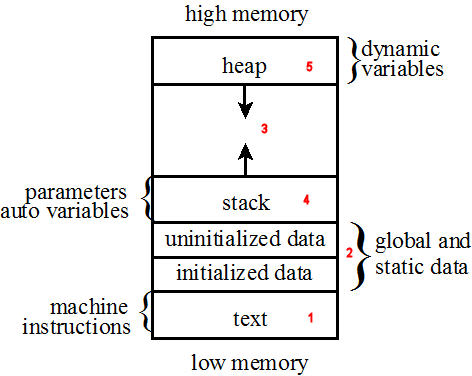
\includegraphics[scale=0.5]{OOPandUML/functional_memory_organization}
        \label{fig:functional_memory_organization}
        \caption{Functional memory organization of a running program}
    \end{center}
\end{figure}

\toclessnparagraph{Text}
This area contains machine instructions (i.e. the executable 
code). \textbf{Global} and \textbf{static} variables are typically 
allocated at program startup. \textbf{Stack} contains all the automatic 
variables. \textbf{Heap} is meant to allocate the memory for the dynamic 
variables through the \textbf{\texttt{new}} and \textbf{\texttt{delete}} 
operators. The space in between is allocated by the operating system but 
not used, and is meant to let both the heap and stack grow.

\toclessnparagraph{Stack}
This is a simple LIFO (last in, first out) data structure which must 
support at least the \textbf{push} and \textbf{pop} operations. Even 
though a stack only allows accesses at the top, it is easy to implement 
and fast to execute push and pop operations.

\toclessnparagraph{Heap}
This is a more flexible data structure, which allows programs to 
allocate or deallocate memory anywhere and in any convenient order. This 
might cause hole in the heap, i.e. unallocated memory surrounded by 
allocated memory.
\newline
The only restriction for the heap is that memory can be allocated in 
a contiguous block of memory large enough to satisfy the request with a 
single chunk of memory. This restriction has two effects: it requires 
the operating system to scan the heap until a contiguous block is found, 
and to coalesce adjacent blocks of memory returned by the program.
\newline
Side effect is that the operation on the heap are slower than the 
operations on the stack.

\subsection{Memory Allocation and Deallocation in C}
\subsubsection{\texttt{\href{https://en.cppreference.com/w/c/memory/malloc}{malloc}}}
\subsubsection{\texttt{\href{https://en.cppreference.com/w/c/memory/free}{free}}}

\subsection{Memory Allocation and Deallocation in C++}
\subsubsection{\texttt{\href{https://en.cppreference.com/w/cpp/language/new}{new expression}}}
\subsubsection{\texttt{\href{https://en.cppreference.com/w/cpp/language/delete}{delete expression}}}




\newpage
\printbibsection{subbibintoc}{memorymanagement}{Memory Management Bibliography}
\chapter{Smart Pointers}
\label{chap:smartpoint}

\section{Smart Pointers in C++}
See~\cite{cppreference-dynmemmanagement}.
\newline
\highlight{Smart pointers} enable \highlightit{automatic, exception-safe, object 
lifetime management}.
\newline
Generally speaking, a smart pointer is a \highlightit{data type whose value 
can be used like a pointer}, with the \highlightit{additional feature of 
memory management}, that \highlightit{frees the memory when it is no longer used}.
\newline
A smart pointer should therefore be used any time 
the ownership of memory needs to be tracked.

\toclessnparagraph{Which pointer?}
\begin{itemize}
    \item Prefer \texttt{std::unique\char`_ptr} --- exclusive ownership, zero overhead vs a raw pointer + delete.
    \item Use \texttt{std::shared\char`_ptr} only when ownership is genuinely shared.
    \item Use \texttt{std::weak\char`_ptr} to observe a \texttt{shared\char`_ptr}-managed object 
          without extending its lifetime (break cycles, caches).
    \item Do not use \texttt{std::auto\char`_ptr} (removed from the language).
\end{itemize}

\newpage
%% Unique Pointer
\subsection{\texttt{std::unique\char`_ptr}}
\label{subsec:unique-ptr}
See~\cite{cppreference-uniqueptr}.
\newline
\highlighttt{std::unique\char`_ptr} is a smart pointer that \highlightit{owns and manages} 
another object through a pointer and \highlightit{disposes of} that object 
\highlightit{when} the \highlighttt{std::unique\char`_ptr} goes \highlightit{out of scope}.
\newline
The object is disposed of, using the associated deleter when either 
of the following happens:
\begin{itemize}
    \item the managing \texttt{std::unique\char`_ptr} object is \highlightit{destroyed}
    \item the managing \texttt{std::unique\char`_ptr} object is \highlightit{assigned 
          another pointer} via \texttt{operator=} or \texttt{reset()}. 
\end{itemize}

\toclessnparagraph{Notes}
Only a \highlight{\textbf{non-const} \texttt{std::unique\char`_ptr}} can 
\highlightit{transfer the ownership} of the managed object to \highlight{\textbf{another} 
\texttt{std::unique\char`_ptr}} (via move).
\newline
If an object's lifetime is managed by a 
\highlight{\textbf{const} \texttt{std::unique\char`_ptr}}, it is \highlight{limited to 
the scope} in which the pointer was created.

\highlight{\texttt{std::unique\char`_ptr}} is commonly used to \highlight{manage} the \highlight{lifetime 
of objects}, including:
\begin{itemize}
    \item providing \highlight{exception safety} to classes and functions 
          that handle objects with dynamic lifetime, 
          by \highlight{guaranteeing deletion} on both normal exit and 
          exit through exception 
    \item \highlight{passing ownership} of uniquely-owned objects with 
          dynamic lifetime into functions 
    \item \highlight{acquiring ownership} of uniquely-owned objects 
          with dynamic lifetime from functions 
    \item as the element type in move-aware containers, 
          such as \texttt{std::vector}, which hold pointers to 
          dynamically-allocated objects
          (e.g.\ if \highlight{polymorphic behavior} is desired).             
\end{itemize}

\highlighttt{std::unique\char`_ptr} may be constructed for an
\highlight{incomplete type} \texttt{T}, such as to facilitate the use as a handle 
in the \highlight{PImpl idiom} (Chapter~\ref{chap:idioms}).

\begin{lstlisting}[language=C++]
#include <memory>

struct Widget { void draw(); };

std::unique_ptr<Widget> p = std::make_unique<Widget>();
p->draw();

std::unique_ptr<Widget> q = std::move(p);  // ownership transferred
// p == nullptr
\end{lstlisting}

\toclessnparagraph{\texttt{std::make\char`_unique}}
Prefer \texttt{std::make\char`_unique} (C++14) over \texttt{new} 
(see~\cite{cppreference-make-unique}; also~\S\ref{sec:std-make-unique}): no naked \texttt{new}, 
less repetition of the type name, and better exception safety when 
building function arguments.
\begin{lstlisting}[language=C++]
foo(std::make_unique<T>(), function_that_throws(), std::make_unique<T>());
\end{lstlisting}

\toclessnparagraph{Arrays and custom deleters}
Array form uses \texttt{delete[]}. A custom deleter is useful for C APIs, pools, and \texttt{FILE*}.
\begin{lstlisting}[language=C++]
// array form: uses delete[]
auto buf = std::make_unique<int[]>(1024);

// custom deleter (e.g. C API / pool / FILE*)
std::unique_ptr<FILE, decltype(&std::fclose)> f{
    std::fopen("data.bin", "rb"), &std::fclose};
\end{lstlisting}

\toclessnparagraph{Member types}
\begin{table}[H]
    \begin{tabularx}{\textwidth}{|l|X|}
        \cline{1-2}
        pointer & Must satisfy \href{https://en.cppreference.com/w/cpp/named_req/NullablePointer}{NullablePtr}\\
        \cline{1-2}
        element\char`_type 
        & T, the type of the object managed by this \texttt{std::unique\char`_ptr}\\
        \cline{1-2}
        \multirow{2}{*}{deleter\char`_type}
        & Deleter, the function object or lvalue reference \\ 
        & to function or to function object, to be called from the destructor \\
        \cline{1-2}
    \end{tabularx}
\end{table}

\toclessnparagraph{Member functions}
\begin{table}[H]
    \begin{tabularx}{\textwidth}{|l|X|}
        \cline{1-2}
        \href{https://en.cppreference.com/w/cpp/memory/unique_ptr/unique_ptr}{constructor}
        & constructs a new \texttt{unique\char`_ptr}\\
        \cline{1-2}
        \href{https://en.cppreference.com/w/cpp/memory/unique_ptr/\%7Eunique_ptr}{destructor}
        & destructs the managed object if such is present\\
        \cline{1-2}
        \href{https://en.cppreference.com/w/cpp/memory/unique_ptr/operator\%3D}{operator=}
        & assigns the \texttt{unique\char`_ptr} (moves ownership)\\
        \cline{1-2}
    \end{tabularx}
\end{table}

\toclessnparagraph{Modifiers}
\begin{table}[H]
    \begin{tabularx}{\textwidth}{|l|X|}
        \cline{1-2}
        \href{https://en.cppreference.com/w/cpp/memory/unique_ptr/release}{release}
        & releases ownership and returns the raw pointer (caller must delete)\\
        \cline{1-2}
        \href{https://en.cppreference.com/w/cpp/memory/unique_ptr/reset}{reset}
        & replaces the managed object (deletes the old one if any)\\
        \cline{1-2}
        \href{https://en.cppreference.com/w/cpp/memory/unique_ptr/swap}{swap}
        & swaps the managed objects with another \texttt{unique\char`_ptr}\\
        \cline{1-2}
    \end{tabularx}
\end{table}

\toclessnparagraph{Observers}
\begin{table}[H]
    \begin{tabularx}{\textwidth}{|l|X|}
        \cline{1-2}
        \href{https://en.cppreference.com/w/cpp/memory/unique_ptr/get}{get}
        & returns a pointer to the managed object\\
        \cline{1-2}
        \href{https://en.cppreference.com/w/cpp/memory/unique_ptr/get_deleter}{get\char`_deleter}
        & returns the deleter that is used for destruction of the managed object\\
        \cline{1-2}
        \href{https://en.cppreference.com/w/cpp/memory/unique_ptr/operator_bool}{operator bool}
        & checks if there is an associated managed object\\
        \cline{1-2}
    \end{tabularx}
\end{table}

\toclessnparagraph{Single-object version, \texttt{unique\char`_ptr$<$T$>$}}
\begin{table}[H]
    \begin{tabularx}{\textwidth}{|l|X|}
        \cline{1-2}
        \multirow{2}{*}{\parbox{4cm}{\href{https://en.cppreference.com/w/cpp/memory/unique_ptr/operator*}{operator*} \\
                                     \href{https://en.cppreference.com/w/cpp/memory/unique_ptr/operator*}{operator->}}} 
                        & dereferences pointer to the managed object \\
                        &  \\
        \cline{1-2}
    \end{tabularx}
\end{table}

\newpage
%% Shared Ptr
\subsection{\texttt{std::shared\char`_ptr}}
\label{subsec:shared-ptr}
See~\cite{cppreference-sharedptr}.
\newline
This is a smart pointer that \highlight{retains shared ownership} of an object 
through a pointer.
\newline
\highlight{Several \texttt{shared\char`_ptr} objects may own the same object}.
\newline
The object is destroyed and its memory deallocated when either of 
the following happens:
\begin{itemize}
    \item the \highlight{last remaining} \texttt{shared\char`_ptr} owning 
          the object \highlight{is destroyed};
    \item the \highlight{last remaining} \texttt{shared\char`_ptr} owning 
          the object is \highlight{assigned another pointer} via \texttt{operator=} or 
          \texttt{reset()}.             
\end{itemize}

A \texttt{std::shared\char`_ptr} can share ownership of an object 
while storing a pointer to another object (aliasing constructor).
\newline
A \texttt{std::shared\char`_ptr} may also own no objects, 
in which case it is called empty (an empty 
\texttt{std::shared\char`_ptr} may have a non-null stored pointer 
if the aliasing constructor was used to create it). 

\toclessnparagraph{\texttt{std::make\char`_shared}}
Prefer \texttt{std::make\char`_shared} (see~\cite{cppreference-make-shared}; 
also~\S\ref{sec:std-make-shared}): 
exception safety, and typically \textbf{one allocation} for control block + object.
\begin{lstlisting}[language=C++]
auto a = std::make_shared<Widget>();
auto b = a;                 // shared ownership; use_count() == 2
a.reset();                  // b still owns the Widget
\end{lstlisting}

Control-block bookkeeping is thread-safe; concurrent mutation of the 
\textit{managed object} is not.

\toclessnparagraph{Member functions}
\begin{table}[H]
    \begin{tabularx}{\textwidth}{|l|X|}
        \cline{1-2}
        \href{https://en.cppreference.com/w/cpp/memory/shared_ptr/shared_ptr}{constructor}
        & constructs a new \texttt{shared\char`_ptr}\\
        \cline{1-2}
        \href{https://en.cppreference.com/w/cpp/memory/shared_ptr/\%7Eshared_ptr}{destructor}
        & decrements the reference count; destroys the object if it reaches zero\\
        \cline{1-2}
        \href{https://en.cppreference.com/w/cpp/memory/shared_ptr/operator\%3D}{operator=}
        & assigns the \texttt{shared\char`_ptr} \\
        \cline{1-2}
    \end{tabularx}
\end{table}    

\toclessnparagraph{Modifiers}
\begin{table}[H]
    \begin{tabularx}{\textwidth}{|l|X|}
        \cline{1-2}
        \href{https://en.cppreference.com/w/cpp/memory/shared_ptr/reset}{reset}
        & replaces the managed object \\
        \cline{1-2}
        \href{https://en.cppreference.com/w/cpp/memory/shared_ptr/swap}{swap}
        & swaps the managed objects \\
        \cline{1-2}
    \end{tabularx}
\end{table} 

\newpage
\toclessnparagraph{Observers}
\begin{table}[H]
    \begin{tabularx}{\textwidth}{|l|X|}
        \cline{1-2}
        \href{https://en.cppreference.com/w/cpp/memory/shared_ptr/get}{get}
        & returns the stored pointer \\
        \cline{1-2}
        \multirow{2}{*}{\parbox{4cm}{\href{https://en.cppreference.com/w/cpp/memory/shared_ptr/operator*}{operator*} \\
                                     \href{https://en.cppreference.com/w/cpp/memory/shared_ptr/operator*}{operator->}}}
        & dereferences the stored pointer \\ 
        & \\
        \cline{1-2}
        \href{https://en.cppreference.com/w/cpp/memory/shared_ptr/operator_at}{operator[]} 
        & provides indexed access to the stored array (C++17) \\
        \cline{1-2}
        \multirow{2}{*}{\href{https://en.cppreference.com/w/cpp/memory/shared_ptr/use_count}{use\char`_count}} 
        & returns the number of \texttt{shared\char`_ptr} objects \\ & referring to the same managed object \\
        \cline{1-2}
        \multirow{2}{*}{\href{https://en.cppreference.com/w/cpp/memory/shared_ptr/unique}{unique}}
        & checks if \texttt{use\char`_count() == 1} \\ 
        & (deprecated in C++17, removed in C++20) \\
        \cline{1-2}
        \href{https://en.cppreference.com/w/cpp/memory/shared_ptr/operator_bool}{operator bool}
        & checks if the stored pointer is not null \\
        \cline{1-2}
        \href{https://en.cppreference.com/w/cpp/memory/shared_ptr/owner_before}{owner\char`_before}
        & provides owner-based ordering of shared pointers \\
        \cline{1-2}
    \end{tabularx}
\end{table} 

\newpage
%% Weak Ptr
\subsection{\texttt{std::weak\char`_ptr}}
\label{subsec:weak-ptr}
See~\cite{cppreference-weakpointer}.
\newline
\texttt{std::weak\char`_ptr} is a smart pointer that holds a non-owning (``weak'') reference 
to an object that is managed by \texttt{std::shared\char`_ptr}. 
It must be converted to \texttt{std::shared\char`_ptr} (via \texttt{lock()}) in order to access 
the referenced object. 
\newline
\texttt{std::weak\char`_ptr} models \highlight{temporary / non-owning} observation: 
it does not keep the object alive, but can detect whether it still exists 
(\texttt{expired()}).

\toclessnparagraph{Breaking cycles}
If two objects each hold a \texttt{shared\char`_ptr} to the other, the reference count 
never reaches zero. Store one side as \texttt{weak\char`_ptr}.
\begin{lstlisting}[language=C++]
struct Node {
    std::shared_ptr<Node> next;   // owning
    std::weak_ptr<Node>   prev;   // non-owning: breaks the cycle
};

auto a = std::make_shared<Node>();
auto b = std::make_shared<Node>();
a->next = b;
b->prev = a;

if (auto p = b->prev.lock()) {    // promote to shared_ptr if still alive
    // use *p
}
\end{lstlisting}

Related: \texttt{std::enable\char`_shared\char`_from\char`_this$<$T$>$} 
(see~\cite{cppreference-enable-shared-from-this}) lets a member function obtain a 
\texttt{shared\char`_ptr} to \texttt{*this} safely when the object is already owned 
by a \texttt{shared\char`_ptr}.
    
\toclessnparagraph{Member functions}
\begin{table}[H]
    \begin{tabularx}{\textwidth}{|l|X|}
        \cline{1-2}
        \href{https://en.cppreference.com/w/cpp/memory/weak_ptr/weak_ptr}{constructor}
        & creates a new \texttt{weak\char`_ptr} \\
        \cline{1-2}
        \href{https://en.cppreference.com/w/cpp/memory/weak_ptr/\%7Eweak_ptr}{destructor}
        & destroys a \texttt{weak\char`_ptr} (does not destroy the managed object) \\
        \cline{1-2}
        \href{https://en.cppreference.com/w/cpp/memory/weak_ptr/operator\%3D}{operator=}
        & assigns a \texttt{weak\char`_ptr} \\
        \cline{1-2}
    \end{tabularx}
\end{table}
    
\toclessnparagraph{Modifiers}
\begin{table}[H]
    \begin{tabularx}{\textwidth}{|l|X|}
        \cline{1-2}
        \href{https://en.cppreference.com/w/cpp/memory/weak_ptr/reset}{reset}
        & releases the weak reference \\
        \cline{1-2}
        \href{https://en.cppreference.com/w/cpp/memory/weak_ptr/swap}{swap}
        & swaps with another \texttt{weak\char`_ptr} \\
        \cline{1-2}
    \end{tabularx}
\end{table}

\newpage
\toclessnparagraph{Observers}
\begin{table}[H]
    \begin{tabularx}{\textwidth}{|l|X|}
        \cline{1-2}
        \href{https://en.cppreference.com/w/cpp/memory/weak_ptr/use_count}{use\char`_count}
        & returns the number of \texttt{shared\char`_ptr} objects that manage the object \\
        \cline{1-2}
        \href{https://en.cppreference.com/w/cpp/memory/weak_ptr/expired}{expired}
        & checks whether the referenced object was already deleted \\
        \cline{1-2}
        \href{https://en.cppreference.com/w/cpp/memory/weak_ptr/lock}{lock}
        & creates a \texttt{shared\char`_ptr} that manages the referenced object (or empty if expired) \\
        \cline{1-2}
        \href{https://en.cppreference.com/w/cpp/memory/weak_ptr/owner_before}{owner\char`_before}
        & provides owner-based ordering of weak pointers \\
        \cline{1-2}
    \end{tabularx}
\end{table}       

\newpage
\subsection{\texttt{std::auto\char`_ptr}}
\label{subsec:auto-ptr}
See~\cite{cppreference-autopointer}.
\newline
\texttt{std::auto\char`_ptr} was an early exclusive-ownership smart pointer. 
Copying it \textbf{transferred} ownership (surprising copy semantics), which 
made it unsafe in standard containers and easy to misuse.
\newline
It was \textbf{deprecated in C++11} and \textbf{removed in C++17}. 
Use \texttt{std::unique\char`_ptr} (move-only) instead.

\newpage
\printbibsection{subbibintoc}{smartpointers}{Smart Pointers Bibliography}
\chapter{Containers}
\label{chap:containers}
\vspace{10.5cm}
The \href{https://en.cppreference.com/w/cpp/container}{Containers library} is a generic collection 
of class templates and algorithms that allow programmers to easily implement 
common data structures like queues, lists and stacks.
\newline
The container classes are:
\begin{itemize}
    \item sequence containers
    \item associative containers, which can be searched in $O(\log{n})$.
    \item unordered associative containers, which can be searched in $O(1)$ on average and in $O(n)$ in the worst one.
\end{itemize}

\section{Links to the CPP Reference documentation}

\subsection{Sequence Containers}
\href{https://en.cppreference.com/w/cpp/container/array}{array}\quad | \quad
\href{https://en.cppreference.com/w/cpp/container/vector}{vector}\quad | \quad
\href{https://en.cppreference.com/w/cpp/container/deque}{deque}\quad | \quad
\href{https://en.cppreference.com/w/cpp/container/forward_{list}}{forward\char`_list}\quad | \quad
\href{https://en.cppreference.com/w/cpp/container/list}{list}

\subsection{Associative Containers}

\href{https://en.cppreference.com/w/cpp/container/set}{set}\quad | \quad
\href{https://en.cppreference.com/w/cpp/container/map}{map}\quad | \quad
\href{https://en.cppreference.com/w/cpp/container/multiset}{multiset}\quad | \quad
\href{https://en.cppreference.com/w/cpp/container/multimap}{multimap}

\subsection{Unordered Associative Containers}

\href{https://en.cppreference.com/w/cpp/container/unordered_set}{unordered\char`_set}\quad | \quad
\href{https://en.cppreference.com/w/cpp/container/unordered_map}{unordered\char`_map}\quad | \quad
\href{https://en.cppreference.com/w/cpp/container/unordered_multiset}{unordered\char`_multiset}\quad | \quad
\href{https://en.cppreference.com/w/cpp/container/unordered_multimap}{unordered\char`_multimap}

\subsection{Container Adaptors}
\href{https://en.cppreference.com/w/cpp/container/stack}{stack}\quad | \quad
\href{https://en.cppreference.com/w/cpp/container/queue}{queue}\quad | \quad
\href{https://en.cppreference.com/w/cpp/container/priority_queue}{priority\char`_queue}\quad | \quad
\href{https://en.cppreference.com/w/cpp/container/flat_set}{flat\char`_set}\quad | \quad
\href{https://en.cppreference.com/w/cpp/container/flat_map}{flat\char`_map}\quad | \quad
\href{https://en.cppreference.com/w/cpp/container/flat_multiset}{flat\char`_multiset}\quad | \quad
\href{https://en.cppreference.com/w/cpp/container/flat_multimap}{flat\char`_multimap}

\section{Containers' Access Time}
\begin{table}[h!t]
    \begin{tabularx}{\textwidth}{X|c|c|c|c}
    %~ \begin{tabular}{l|c|c|c|c}
        \multirow{2}{*}{Associative Container} & \multirow{2}{*}{Sorted} & \multirow{2}{*}{Value} & Multiple Identical & \multirow{2}{*}{Access Time} \\
                                               &        &       & Keys & \\
        \hline
        \texttt{std::set} & yes & no & no & logarithmic \\
        \texttt{std::unordered\char`_set} & no & no & no & constant \\
        \texttt{std::map} & yes & yes & no & logarithmic \\
        \texttt{std::unordered\char`_map} & no & yes & no & constant \\
        \texttt{std::multiset} & yes & no & yes & logarithmic\\
        \texttt{std::unordered\char`_multiset} & no & no & yes & constant\\
        \texttt{std::multimap} & yes & yes & yes & logarithmic\\
        \texttt{std::unordered\char`_multimap} & no & yes & yes & constant\\
    \end{tabularx}
    %~ \end{tabular}
\end{table}
\newpage
\section{Invalidation of Iterators and References}
\begin{table}[ht]
\footnotesize{}
    \begin{tabular}{|c|c|c|c|c|c|c|}
        \hline
        \multirow{2}{*}{Category} & \multirow{2}{*}{Container} & \multicolumn{2}{c|}{Valid after \textbf{insertion}} & \multicolumn{2}{c|}{Valid after \textbf{erasure}} &  \multirow{2}{*}{Conditionality} \\
                                &                              &iterators&reference&iterators&reference& \\
        \hline
        \multirow{10}{*}{\shortstack{Sequence\\Containers}} & array & \multicolumn{2}{c|}{ N/A } & \multicolumn{2}{c|}{ N/A } & \\
        \cline{2-7}
                                                            & \multirow{5}{*}{vector}            & \multicolumn{2}{c|}{No}    & \multicolumn{2}{c|}{N/A} & Insertion changed capacity\\
        \cline{3-7}
                                                            &                                    & \multicolumn{2}{c|}{\multirow{3}{*}{Yes}}      &  \multicolumn{2}{c|}{\multirow{3}{*}{Yes}}  & \multirow{3}{*}{\shortstack{Before modified element(s)\\(for insertion only if capacity\\didn't change) }} \\
                                                            &                                    &  \multicolumn{2}{c|}{}                         &  \multicolumn{2}{c|}{}                       &  \\
                                                            &                                    &  \multicolumn{2}{c|}{}                         &  \multicolumn{2}{c|}{}                       &  \\
        \cline{3-7}
                                                            &                                    &  \multicolumn{2}{c|}{No}                       &  \multicolumn{2}{c|}{No}                     & At or after modified element(s) \\
        \cline{2-7}
                                                            & \multirow{2}{*}{deque} & \multirow{2}{*}{No} & Yes& \multicolumn{2}{c|}{Yes, but erased one(s)} & Modified first or last element \\
        \cline{4-7}
                                                            & & &No& \multicolumn{2}{c|}{No} & Modified middle only \\
        \cline{2-7}
                                                            & list & \multicolumn{2}{c|}{Yes} & \multicolumn{2}{c|}{Yes, but erased one(s)} & \\
        \cline{2-7}
                                                            & forward\char`_list & \multicolumn{2}{c|}{Yes} & \multicolumn{2}{c|}{Yes, but erased one(s)} & \\
        \cline{1-7}

        \multirow{4}{*}{\shortstack{Associative\\Containers}} & set & \multicolumn{2}{c|}{\multirow{4}{*}{Yes}}& \multicolumn{2}{c|}{\multirow{4}{*}{Yes, but erased one(s)}} & \\
                                                              & multiset & \multicolumn{2}{c|}{} & \multicolumn{2}{c|}{}& \\
                                                              & map & \multicolumn{2}{c|}{} & \multicolumn{2}{c|}{} & \\
                                                              & multimap & \multicolumn{2}{c|}{} & \multicolumn{2}{c|}{} & \\
        \cline{1-7}
        \multirow{4}{*}{\shortstack{Unordered\\associative\\Containers}} & unordered\char`_set & \multirow{2}{*}{No}& \multirow{4}{*}{Yes}& \multicolumn{2}{c|}{\multirow{2}{*}{N/A}} & \multirow{2}{*}{Insertion caused rehash}\\
                                                              & unordered\char`_multiset & & & \multicolumn{2}{c|}{} &  \\
        \cline{3-3}\cline{5-7}
                                                              & unordered\char`_map &\multirow{2}{*}{Yes} & & \multicolumn{2}{c|}{\multirow{2}{*}{Yes, but erased one(s)}} & \multirow{2}{*}{No rehash} \\
                                                              & unordered\char`_multimap & & & \multicolumn{2}{c|}{} &\\
        \cline{1-7}
    \end{tabular}
    \label{tab:iterator-reference-validity}
\end{table}
\normalsize

\section{C++23 New Container Adaptors}
\subsection{Containers}
With C++23, the following four Container Adaptors were introduced:
\begin{table}[h!t]
    \begin{tabularx}{\textwidth}{|l|X|}
    %~ \textbf{C++98} & \texttt{std::map}, \texttt{std::set}, \texttt{std::multimap}, \texttt{std::multiset} \\
    %~ \hline
    %~ \multirow{2}{*}{\textbf{C++11}} 
    %~ & \texttt{std::unordered\char`_map}, \texttt{std::unordered\char`_set} \\
    %~ & \texttt{std::unordered\char`_multimap}, \texttt{std::unordered\char`_multiset} \\
    \hline
    {\textbf{C++23}} & \texttt{flat\char`_map}, \quad \texttt{flat\char`_multimap}, 
                       \quad \texttt{flat\char`_set}, \quad \texttt{flat\char`_multiset} \\
    \hline
    \end{tabularx}
\end{table}

\newpage{}

\newpage
\printbibsection{subbibintoc}{containers}{Containers Bibliography}
\chapter{Concurrency}
\label{chap:concurrency}
See~\cite{cppreference-thread},~\cite{cppreference-memory-order}.
\newline
C++ includes built-in support for threads, atomic operations, mutual exclusion, 
condition variables, and futures. Deeper formal memory-model material lives in 
Chapter~\ref{chap:memorymodel}; this chapter is the library map plus usage notes.
\newline
%%% Paragraph
\section{Threads}
\label{sec:threads}
A \texttt{std::thread} is the C++ handle for an OS thread of execution. Threads in the 
same process \highlight{share the address space}: that is why they communicate cheaply 
through memory, and why unsynchronized shared writes are data races 
(Chapter~\ref{chap:memorymodel}).
\begin{table}[H]
    \begin{tabularx}{\textwidth}{|l|X|}
        \cline{1-2}
        \href{https://en.cppreference.com/w/cpp/thread/thread}{thread}
        & manages a separate thread \\
        \cline{1-2}
        \href{https://en.cppreference.com/w/cpp/thread/jthread}{jthread} 
        & thread with support for auto-joining and cooperative stop (C++20) \\
        \cline{1-2}   
    \end{tabularx}
\end{table}

\toclessnparagraph{Process vs thread (C++)}
\begin{itemize}
    \item A \textbf{process} is an OS instance of a program with its own address space.
    \item A \textbf{thread} is a unit of execution \emph{inside} a process; threads of the 
          same process share memory (hence data races if unsynchronized).
    \item \texttt{std::thread} must be \texttt{join()}ed or \texttt{detach()}ed before 
          destruction, or \texttt{std::terminate} is called --- a common production footgun.
    \item Prefer \texttt{std::jthread} when you can: it joins on destruction and can 
          receive a stop token (C++20).
\end{itemize}
\textbf{Noise / failure modes:} leaking joinable threads at shutdown; oversubscribing 
cores (context-switch jitter) when a thread pool would do; using threads when a 
single-threaded reactor + queues is simpler for I/O.
\par\noindent\textbf{Interview tip:} join-or-detach before destruction; prefer 
\texttt{jthread} when you can explain the stop token.

\begin{lstlisting}[language=C++]
#include <iostream>
#include <thread>
#include <string>

void task1(std::string msg) {
    std::cout << "task1 says: " << msg << '\n';
}

int main() {
    std::thread t1(task1, "Hello");  // starts running
    // ... other work on this thread ...
    t1.join();                       // wait for completion
}
\end{lstlisting}

\subsection{Functions managing the current thread}
\vspace{-8truemm}
These APIs act on the \emph{calling} thread. On a latency path, sleeping and yielding 
are how you \highlight{donate the core} back to the scheduler --- useful for fairness, 
harmful if you needed busy-poll determinism.
\begin{table}[H]
    \begin{tabularx}{\textwidth}{|l|X|}
        \cline{1-2}
        \href{https://en.cppreference.com/w/cpp/thread/yield}{yield} 
        & hints the implementation to reschedule; may be a no-op; not a lock substitute \\
        \cline{1-2}
        \href{https://en.cppreference.com/w/cpp/thread/get_id}{get\char`_id} 
        & returns the id of the current thread \\
        \cline{1-2}
        \href{https://en.cppreference.com/w/cpp/thread/sleep_for}{sleep\char`_for} 
        & blocks the current thread for at least the given duration (wake-up jitter) \\
        \cline{1-2}
        \href{https://en.cppreference.com/w/cpp/thread/sleep_until}{sleep\char`_until} 
        & blocks until a time point \\
        \cline{1-2}
    \end{tabularx}
\end{table}
\textbf{Noise removed by \emph{not} sleeping on the hot path:} wake-up delay and 
unpredictable reschedule time. Prefer condition variables / queues when you must wait; 
prefer busy poll only on isolated cores (Chapter~\ref{chap:lowlatency}).
\par\noindent\textbf{Interview tip:} \texttt{yield} is a hint, not a lock; 
\texttt{sleep\char`_for} is wake-up jitter you chose.
%%% Subsection

\section{Atomicity}
\subsection{Atomic operations}
Fine-grained concurrent updates without a mutex. Each atomic operation is 
indivisible with respect to other atomic operations on the \emph{same} object. 
Atomic objects are 
\href{https://en.cppreference.com/w/cpp/language/memory_model#Threads_and_data_races}{free of data races}
on that object --- that is the race/UB noise they remove compared to a plain 
\texttt{int} shared by two threads.
\newline
Atomics do \emph{not} automatically make multi-word invariants safe; you still choose 
a \texttt{memory\char`_order} (Section~\ref{subsec:memory-order}) so publishes become 
visible in the order you intend.
\par\noindent\textbf{Interview tip:} atomic on one word $\neq$ atomic on a struct of 
several fields --- that still needs a mutex or a carefully designed protocol.

\begin{lstlisting}[language=C++]
std::atomic<int> counter{0};
// concurrent increments are data-race-free:
counter.fetch_add(1, std::memory_order_relaxed);
\end{lstlisting}
%~ \newpage
%%% Paragraph
\subsection{Atomic types}
\vspace{-8truemm}
\texttt{std::atomic<T>} wraps a value so loads/stores/RMWs are atomic. Prefer it for 
flags, counters, and single-word handoffs. \texttt{atomic\char`_ref} overlays atomic 
ops on an existing non-atomic object (lifetime/alignment rules apply) --- useful when 
you cannot change the storage type.
\begin{table}[H]
    \begin{tabularx}{\textwidth}{|l|X|}
        \cline{1-2}
        \multirow{2}{*}{\href{https://en.cppreference.com/w/cpp/atomic/atomic}{atomic}} 
        & atomic class template and specializations for \\
        & bool, integral, and pointer types \\
        \cline{1-2}
        \href{https://en.cppreference.com/w/cpp/atomic/atomic_ref}{atomic\char`_ref}
        & provides atomic operations on non-atomic objects \\
        \cline{1-2}
    \end{tabularx}
\end{table}
Check \texttt{is\char`_lock\char`_free} when you care: some wide types fall back to 
internal locks, which reintroduces contention noise you thought you avoided.
\par\noindent\textbf{Interview tip:} ask whether the atomic is lock-free on the target 
ABI before claiming a lock-free design.
%%% Paragraph

\subsection{Operations on atomic types}
\vspace{-8truemm}
%~ \begin{table}[H]
    %~ \begin{adjustbox}{width=1.1\columnwidth,left}
    %~ \begin{tabular}{|l|l|}
        %~ \cline{1-2}
        %~ \href{https://en.cppreference.com/w/cpp/atomic/atomic_is_lock_free}{atomic\char`_is\char`_lock\char`_free} 
        %~ & checks if the atomic type's operations are lock-free \\
        %~ \cline{1-2}
        %~ \multirow{2}{*}{\parbox{4cm}{\href{https://en.cppreference.com/w/cpp/atomic/atomic_store}{atomic\char`_store} \\ 
                                     %~ \href{https://en.cppreference.com/w/cpp/atomic/atomic_store}{atomic\char`_store\char`_explicit}}}
                         %~ & atomically replaces the value of the atomic object  \\
                         %~ & with a non-atomic argument \\
        %~ \cline{1-2}

        %~ \multirow{2}{*}{\parbox{4cm}{\href{https://en.cppreference.com/w/cpp/atomic/atomic_load}{atomic\char`_load} \\
                                     %~ \href{https://en.cppreference.com/w/cpp/atomic/atomic_load}{atomic\char`_load\char`_explicit}}}
                       %~ & atomically obtains the value stored \\
                       %~ & in an atomic object \\
       %~ \cline{1-2}
       %~ \multirow{2}{*}{\parbox{4.5cm}{\href{https://en.cppreference.com/w/cpp/atomic/atomic_exchange}{atomic\char`_exchange} \\ 
                                      %~ \href{https://en.cppreference.com/w/cpp/atomic/atomic_exchange}{atomic\char`_exchange\char`_explicit}}}
                       %~ &  atomically replaces the value of the atomic object with non-atomic argument\\
                       %~ &  and returns the old value of the atomic\\
        %~ \cline{1-2}
        %~ \multirow{4}{*}{\parbox{7.5cm}{\href{https://en.cppreference.com/w/cpp/atomic/atomic_compare_exchange}{atomic\char`_compare\char`_exchange\char`_weak} \\
                                       %~ \href{https://en.cppreference.com/w/cpp/atomic/atomic_compare_exchange}{atomic\char`_compare\char`_exchange\char`_weak\char`_explicit} \\ 
                                       %~ \href{https://en.cppreference.com/w/cpp/atomic/atomic_compare_exchange}{atomic\char`_compare\char`_exchange\char`_strong} \\ 
                                       %~ \href{https://en.cppreference.com/w/cpp/atomic/atomic_compare_exchange}{atomic\char`_compare\char`_exchange\char`_strong\char`_explicit}}}
                        %~ & \\
                        %~ & atomically compares the value of the atomic object with non-atomic argument \\
                        %~ & and performs atomic exchange if equal or atomic load if not \\
                        %~ & \\
        %~ \cline{1-2}
        %~ \multirow{2}{*}{\parbox{4cm}{\href{https://en.cppreference.com/w/cpp/atomic/atomic_fetch_add}{atomic\char`_fetch\char`_add} \\ 
                                     %~ \href{https://en.cppreference.com/w/cpp/atomic/atomic_fetch_add}{atomic\char`_fetch\char`_add\char`_explicit}}}
                        %~ & adds a non-atomic value to an atomic object\\
                        %~ & and obtains the previous value of the atomic \\
        %~ \cline{1-2}
        %~ \multirow{2}{*}{\parbox{4cm}{\href{https://en.cppreference.com/w/cpp/atomic/atomic_fetch_sub}{atomic\char`_fetch\char`_sub} \\ 
                                     %~ \href{https://en.cppreference.com/w/cpp/atomic/atomic_fetch_sub}{atomic\char`_fetch\char`_sub\char`_explicit}}}
                        %~ & subtracts a non-atomic value from an atomic object\\
                        %~ & and obtains the previous value of the atomic\\
        %~ \cline{1-2}
        %~ \multirow{2}{*}{\parbox{4cm}{\href{https://en.cppreference.com/w/cpp/atomic/atomic_fetch_and}{atomic\char`_fetch\char`_and} \\
                                     %~ \href{https://en.cppreference.com/w/cpp/atomic/atomic_fetch_and}{atomic\char`_fetch\char`_and\char`_explicit}}}
                        %~ & replaces the atomic object with the result of bitwise AND with a non-atomic argument\\
                        %~ & and obtains the previous value of the atomic\\
        %~ \cline{1-2}
        %~ \multirow{2}{*}{\parbox{4cm}{\href{https://en.cppreference.com/w/cpp/atomic/atomic_fetch_or}{atomic\char`_fetch\char`_or} \\
                                     %~ \href{https://en.cppreference.com/w/cpp/atomic/atomic_fetch_or}{atomic\char`_fetch\char`_or\char`_explicit}}}
                        %~ & replaces the atomic object with the result of bitwise OR with a\\
                        %~ & a non-atomic argument and obtains the previous value of the atomic \\
        %~ \cline{1-2}
        %~ \multirow{2}{*}{\parbox{4cm}{\href{https://en.cppreference.com/w/cpp/atomic/atomic_fetch_xor}{atomic\char`_fetch\char`_xor} \\
                                     %~ \href{https://en.cppreference.com/w/cpp/atomic/atomic_fetch_xor}{atomic\char`_fetch\char`_xor\char`_explicit}}}
                        %~ & blocks the thread until notified and the atomic value changes \\
                        %~ & \\
        %~ \cline{1-2}
        %~ \multirow{2}{*}{\parbox{4cm}{\href{https://en.cppreference.com/w/cpp/atomic/atomic_wait}{atomic\char`_wait} \\
                                     %~ \href{https://en.cppreference.com/w/cpp/atomic/atomic_wait}{atomic\char`_wait\char`_explicit}}}
                        %~ & replaces the atomic object with the result of bitwise XOR with a non-atomic argument \\
                        %~ & and obtains the previous value of the atomic \\
        %~ \cline{1-2}
        %~ \href{https://en.cppreference.com/w/cpp/atomic/atomic_notify_one}{atomic\char`_notify\char`_one} 
        %~ & notifies a thread blocked in \texttt{atomic\char`_wait} \\
        %~ \cline{1-2}
        %~ \href{https://en.cppreference.com/w/cpp/atomic/atomic_notify_all}{atomic\char`_notify\char`_all} 
        %~ & notifies all threads blocked in \texttt{atomic\char`_wait} \\
        %~ \cline{1-2}
    %~ \end{tabular}
    %~ \end{adjustbox}
%~ \end{table}
\begin{table}[H]
    %~ \begin{adjustbox}{width=1.1\columnwidth,left}
    \begin{tabularx}{\textwidth}{|l|X|}
        \cline{1-2}
        \href{https://en.cppreference.com/w/cpp/atomic/atomic_is_lock_free}{atomic\char`_is\char`_lock\char`_free} 
        & checks if the atomic type's operations are lock-free \\
        \cline{1-2}
        \multirow{2}{*}{\parbox{4cm}{\href{https://en.cppreference.com/w/cpp/atomic/atomic_store}{atomic\char`_store} \\ 
                                     \href{https://en.cppreference.com/w/cpp/atomic/atomic_store}{atomic\char`_store\char`_explicit}}}
                         & atomically replaces the value of the atomic object  \\
                         & with a non-atomic argument \\
        \cline{1-2}

        \multirow{2}{*}{\parbox{4cm}{\href{https://en.cppreference.com/w/cpp/atomic/atomic_load}{atomic\char`_load} \\
                                     \href{https://en.cppreference.com/w/cpp/atomic/atomic_load}{atomic\char`_load\char`_explicit}}}
                       & atomically obtains the value stored \\
                       & in an atomic object \\
       \cline{1-2}
       \multirow{2}{*}{\parbox{4.5cm}{\href{https://en.cppreference.com/w/cpp/atomic/atomic_exchange}{atomic\char`_exchange} \\ 
                                      \href{https://en.cppreference.com/w/cpp/atomic/atomic_exchange}{atomic\char`_exchange\char`_explicit}}}
                       &  atomically replaces the value of the atomic object with non-atomic argument\\
                       &  and returns the old value of the atomic\\
        \cline{1-2}
        \multirow{4}{*}{\parbox{7.5cm}{\href{https://en.cppreference.com/w/cpp/atomic/atomic_compare_exchange}{atomic\char`_compare\char`_exchange\char`_weak} \\
                                       \href{https://en.cppreference.com/w/cpp/atomic/atomic_compare_exchange}{atomic\char`_compare\char`_exchange\char`_weak\char`_explicit} \\ 
                                       \href{https://en.cppreference.com/w/cpp/atomic/atomic_compare_exchange}{atomic\char`_compare\char`_exchange\char`_strong} \\ 
                                       \href{https://en.cppreference.com/w/cpp/atomic/atomic_compare_exchange}{atomic\char`_compare\char`_exchange\char`_strong\char`_explicit}}}
                        & \\
                        & atomically compares the value of the atomic object with non-atomic argument \\
                        & and performs atomic exchange if equal or atomic load if not \\
                        & \\
        \cline{1-2}
        \multirow{2}{*}{\parbox{4cm}{\href{https://en.cppreference.com/w/cpp/atomic/atomic_fetch_add}{atomic\char`_fetch\char`_add} \\ 
                                     \href{https://en.cppreference.com/w/cpp/atomic/atomic_fetch_add}{atomic\char`_fetch\char`_add\char`_explicit}}}
                        & adds a non-atomic value to an atomic object\\
                        & and obtains the previous value of the atomic \\
        \cline{1-2}
        \end{tabularx}
        \end{table}
        
        \begin{table}[H]
    %~ \begin{adjustbox}{width=1.1\columnwidth,left}
        \begin{tabularx}{\textwidth}{|l|X|}
        \cline{1-2}
        \multirow{2}{*}{\parbox{4cm}{\href{https://en.cppreference.com/w/cpp/atomic/atomic_fetch_sub}{atomic\char`_fetch\char`_sub} \\ 
                                     \href{https://en.cppreference.com/w/cpp/atomic/atomic_fetch_sub}{atomic\char`_fetch\char`_sub\char`_explicit}}}
                        & subtracts a non-atomic value from an atomic object\\
                        & and obtains the previous value of the atomic\\
        \cline{1-2}
        \multirow{2}{*}{\parbox{4cm}{\href{https://en.cppreference.com/w/cpp/atomic/atomic_fetch_and}{atomic\char`_fetch\char`_and} \\
                                     \href{https://en.cppreference.com/w/cpp/atomic/atomic_fetch_and}{atomic\char`_fetch\char`_and\char`_explicit}}}
                        & replaces the atomic object with the result of bitwise AND with a non-atomic argument\\
                        & and obtains the previous value of the atomic\\
        \cline{1-2}
        \multirow{2}{*}{\parbox{4.5cm}{\href{https://en.cppreference.com/w/cpp/atomic/atomic_fetch_or}{atomic\char`_fetch\char`_or} \\
                                     \href{https://en.cppreference.com/w/cpp/atomic/atomic_fetch_or}{atomic\char`_fetch\char`_or\char`_explicit}}}
                        & replaces the atomic object with the result of bitwise OR with a\\
                        & non-atomic argument and obtains the previous value of the atomic \\
        \cline{1-2}
        \multirow{2}{*}{\parbox{4cm}{\href{https://en.cppreference.com/w/cpp/atomic/atomic_fetch_xor}{atomic\char`_fetch\char`_xor} \\
                                     \href{https://en.cppreference.com/w/cpp/atomic/atomic_fetch_xor}{atomic\char`_fetch\char`_xor\char`_explicit}}}
                        & replaces the atomic object with the result of bitwise XOR with a non-atomic argument \\
                        & and obtains the previous value of the atomic \\
        \cline{1-2}
        \multirow{2}{*}{\parbox{4cm}{\href{https://en.cppreference.com/w/cpp/atomic/atomic_wait}{atomic\char`_wait} \\
                                     \href{https://en.cppreference.com/w/cpp/atomic/atomic_wait}{atomic\char`_wait\char`_explicit}}}
                        & blocks the thread until notified and the atomic value changes \\
                        & \\
        \cline{1-2}
        \href{https://en.cppreference.com/w/cpp/atomic/atomic_notify_one}{atomic\char`_notify\char`_one} 
        & notifies a thread blocked in \texttt{atomic\char`_wait} \\
        \cline{1-2}
        \href{https://en.cppreference.com/w/cpp/atomic/atomic_notify_all}{atomic\char`_notify\char`_all} 
        & notifies all threads blocked in \texttt{atomic\char`_wait} \\
        \cline{1-2}
    \end{tabularx}
    %~ \end{adjustbox}
\end{table}

\newpage
\subsection{Flag type and operations}
\vspace{-8truemm}
\begin{table}[H]
    \begin{tabularx}{\textwidth}{|l|X|}
        \cline{1-2}
        \href{https://en.cppreference.com/w/cpp/atomic/atomic_flag}{atomic\char`_flag} 
              & the lock-free boolean atomic type \\
        \cline{1-2}
        \multirow{2}{*}{\parbox{6cm}{\href{https://en.cppreference.com/w/cpp/atomic/atomic_flag_test_and_set}{atomic\char`_flag\char`_test\char`_and\char`_set} \\
                                     \href{https://en.cppreference.com/w/cpp/atomic/atomic_flag_test_and_set}{atomic\char`_flag\char`_test\char`_and\char`_set\char`_explicit}}}
                        & atomically sets the flag to true and returns its previous \\
                        & value\\
        \cline{1-2}
        \multirow{2}{*}{\parbox{4cm}{\href{https://en.cppreference.com/w/cpp/atomic/atomic_flag_clear}{atomic\char`_flag\char`_clear} \\
                                     \href{https://en.cppreference.com/w/cpp/atomic/atomic_flag_clear}{atomic\char`_flag\char`_clear\char`_explicit}}}
                        & atomically sets the value of the flag to false\\
                        &  \\
        \cline{1-2}
        \multirow{2}{*}{\parbox{4cm}{\href{https://en.cppreference.com/w/cpp/atomic/atomic_flag_test}{atomic\char`_flag\char`_test} \\ 
                                        \href{https://en.cppreference.com/w/cpp/atomic/atomic_flag_test}{atomic\char`_flag\char`_test\char`_explicit}}}
                        & atomically returns the value of the flag \\
                        & \\
        \cline{1-2}
        \multirow{2}{*}{\parbox{4cm}{\href{https://en.cppreference.com/w/cpp/atomic/atomic_flag_wait}{atomic\char`_flag\char`_wait} \\ 
                                     \href{https://en.cppreference.com/w/cpp/atomic/atomic_flag_wait}{atomic\char`_flag\char`_wait\char`_explicit}}}
                        & blocks the thread until notified and the flag changes \\
                        & \\
        \cline{1-2}
        \href{https://en.cppreference.com/w/cpp/atomic/atomic_flag_notify_one}{atomic\char`_flag\char`_notify\char`_one} 
        & notifies a thread blocked in atomic\char`_flag\char`_wait \\
        \cline{1-2}
        \href{https://en.cppreference.com/w/cpp/atomic/atomic_flag_notify_all}{atomic\char`_flag\char`_notify\char`_all} 
        & notifies all threads blocked in atomic\char`_flag\char`_wait \\
        \cline{1-2}
    \end{tabularx}
\end{table}

\subsection{Initialization}
\vspace{-8truemm}
\begin{table}[H]
    \begin{tabularx}{\textwidth}{|l|X|}
        \cline{1-2}
        \href{https://en.cppreference.com/w/cpp/atomic/atomic_init}{atomic\char`_init} 
        & non-atomic initialization of a default-constructed atomic \\
        & object \\
        \cline{1-2}
        \href{https://en.cppreference.com/w/cpp/atomic/ATOMIC_VAR_INIT}{ATOMIC\char`_VAR\char`_INIT} 
        & constant initialization of an atomic variable of static storage duration \\
        \cline{1-2}
        \href{https://en.cppreference.com/w/cpp/atomic/ATOMIC_FLAG_INIT}{ATOMIC\char`_FLAG\char`_INIT} 
        & initializes an \texttt{std::atomic\char`_flag} to false\\
        \cline{1-2}
   \end{tabularx}
\end{table}

\newpage
\subsection{Memory synchronization ordering}
\label{subsec:memory-sync-ordering}
\vspace{-8truemm}
Atomicity alone does not decide \emph{when} other threads see surrounding writes. 
\texttt{memory\char`_order} and fences are how you publish a payload (release) and 
consume it (acquire), or take the blunt \texttt{seq\char`_cst} hammer. Formal 
happens-before material: Chapter~\ref{chap:memorymodel}; choice guide: 
Section~\ref{subsec:memory-order}.
\begin{table}[H]
    \begin{tabularx}{\textwidth}{|l|X|}
         \cline{1-2}
         \href{https://en.cppreference.com/w/cpp/atomic/memory_order}{memory\char`_order} 
         & defines memory ordering constraints for the given atomic operation \\
         \cline{1-2}
         \href{https://en.cppreference.com/w/cpp/atomic/kill_dependency}{kill\char`_dependency} 
         & \small{removes the specified object from the \texttt{memory\char`_order\char`_consume} dependency tree} \\
         \cline{1-2}
         \href{https://en.cppreference.com/w/cpp/atomic/atomic_thread_fence}{atomic\char`_thread\char`_fence} 
         & generic memory order-dependent fence synchronization primitive \\
         \cline{1-2}
         \href{https://en.cppreference.com/w/cpp/atomic/atomic_signal_fence}{atomic\char`_signal\char`_fence} 
         & fence between a thread and a signal handler executed in the same thread \\
         \cline{1-2}
    \end{tabularx}
\end{table}
\textbf{Noise removed by correct ordering:} seeing a flag ``ready'' while the payload 
stores are still invisible (or the opposite reordering bugs on weakly ordered CPUs).
\par\noindent\textbf{Interview tip:} release publishes the payload; acquire consumes it --- 
say that before naming fence APIs.

\subsection{Mutual exclusion}
\label{subsec:mutual-exclusion}
See~\cite{cppreference-mutex}.
\newline
A mutex serializes a critical section: only one owner at a time. That removes data 
races on multi-word invariants atomics alone cannot express --- at the cost of 
possible blocking, priority inversion, and cache-line ping-pong under contention.
\newline
\vspace{-8truemm}
\begin{table}[H]
    \begin{tabularx}{\textwidth}{|l|X|}
        \cline{1-2}
        \href{https://en.cppreference.com/w/cpp/thread/mutex}{mutex} 
        & basic exclusive lock; default choice \\
        \cline{1-2}
        \multirow{2}{*}{\href{https://en.cppreference.com/w/cpp/thread/timed_mutex}{timed\char`_mutex} }
        & exclusive lock with try-lock until a timeout \\
        & (detect / bound wait; do not use as a design default) \\ 
        \cline{1-2}
        \multirow{2}{*}{\href{https://en.cppreference.com/w/cpp/thread/recursive_mutex}{recursive\char`_mutex}} 
        & same thread may lock repeatedly; usually a design smell \\
        & (refactor call graphs instead when possible) \\
        \cline{1-2}
        \multirow{2}{*}{\href{https://en.cppreference.com/w/cpp/thread/recursive_timed_mutex}{recursive\char`_timed\char`_mutex}} 
        & recursive + timeout \\
        & \\
        \cline{1-2}
        \href{https://en.cppreference.com/w/cpp/thread/shared_mutex}{shared\char`_mutex} 
        & many readers or one writer; see below \\
        \cline{1-2}
        \multirow{2}{*}{\href{https://en.cppreference.com/w/cpp/thread/shared_timed_mutex}{shared\char`_timed\char`_mutex}} 
        & shared mutex with timeouts \\
        & \\
        \cline{1-2}
    \end{tabularx}
\end{table}
On a latency-critical core, prefer shrinking the critical section or using a lock-free 
SPSC handoff over adding \texttt{recursive\char`_mutex} / heavy reader--writer machinery.
\par\noindent\textbf{Interview tip:} default to \texttt{mutex}; justify 
\texttt{recursive\char`_mutex} or \texttt{shared\char`_mutex} only with a concrete 
contention story.

\subsection{Generic mutex management}
\vspace{-8truemm}
Always lock with RAII. Raw \texttt{lock()}/\texttt{unlock()} pairs leak the lock on 
exceptions and early returns --- that is the deadlock / stuck-mutex class these 
wrappers remove.
\begin{table}[H]
    \begin{tabularx}{\textwidth}{|l|X|}
        \cline{1-2}
        \href{https://en.cppreference.com/w/cpp/thread/lock_guard}{lock\char`_guard} 
        & simplest scope-based exclusive ownership \\
        \cline{1-2}
        \href{https://en.cppreference.com/w/cpp/thread/scoped_lock}{scoped\char`_lock} 
        & RAII for one or many mutexes; avoids lock-order deadlocks when locking several \\
        \cline{1-2}
        \href{https://en.cppreference.com/w/cpp/thread/unique_lock}{unique\char`_lock} 
        & movable exclusive ownership; required by \texttt{condition\char`_variable::wait} \\
        \cline{1-2}
        \href{https://en.cppreference.com/w/cpp/thread/shared_lock}{shared\char`_lock} 
        & movable shared ownership for \texttt{shared\char`_mutex} \\
        \cline{1-2}
        \multirow{3}{*}{\parbox{4cm}{\href{https://en.cppreference.com/w/cpp/thread/lock_tag_t}{defer\char`_lock\char`_t} \\
                                     \href{https://en.cppreference.com/w/cpp/thread/lock_tag_t}{try\char`_to\char`_lock\char`_t} \\
                                     \href{https://en.cppreference.com/w/cpp/thread/lock_tag_t}{adopt\char`_lock\char`_t}}} 
                        &  \\
                        & tag type used to specify locking strategy  \\
                        &  \\
        \cline{1-2}
        \multirow{3}{*}{\parbox{4cm}{\href{https://en.cppreference.com/w/cpp/thread/lock_tag}{defer\char`_lock} \\
                                     \href{https://en.cppreference.com/w/cpp/thread/lock_tag}{try\char`_to\char`_lock} \\
                                     \href{https://en.cppreference.com/w/cpp/thread/lock_tag}{adopt\char`_lock}}} 
                        &  \\
                        & tag constants used to specify locking strategy  \\
                        &  \\
        \cline{1-2}
    \end{tabularx}
\end{table}
\par\noindent\textbf{Interview tip:} \texttt{lock\char`_guard} by default; 
\texttt{unique\char`_lock} when you need \texttt{wait}; \texttt{scoped\char`_lock} 
when locking more than one mutex.
\newpage
\subsection{Generic locking management}
\vspace{-8truemm}
\begin{table}[H]
    \begin{tabularx}{\textwidth}{|l|X|}
        \cline{1-2}
        \href{https://en.cppreference.com/w/cpp/thread/try_lock}{try\char`_lock} 
        & attempts to obtain ownership of mutexes via repeated calls to \texttt{try\char`_lock} \\
        \cline{1-2}
        \href{https://en.cppreference.com/w/cpp/thread/lock}{lock} 
        & locks specified mutexes, blocks if any are unavailable \\
        \cline{1-2}
    \end{tabularx}
\end{table}

\toclessnparagraph{Mutex vs lock vs semaphore (C++)}
\begin{itemize}
    \item A \textbf{mutex} (\texttt{std::mutex}, \ldots) is the synchronization object 
          threads lock/unlock.
    \item A \textbf{lock wrapper} (\texttt{lock\char`_guard}, \texttt{unique\char`_lock}, 
          \texttt{scoped\char`_lock}) is RAII around a mutex --- prefer these over raw 
          \texttt{lock()}/\texttt{unlock()}.
    \item \texttt{std::mutex} is \emph{not} an OS-wide inter-process lock; for that you 
          need OS primitives / shared-memory named mutexes.
    \item A \textbf{counting semaphore} (\texttt{std::counting\char`_semaphore}, C++20) 
          allows up to $N$ concurrent holders; a binary semaphore is similar to a mutex 
          in spirit but with different API/ownership rules.
    \item Reader/writer access: \texttt{shared\char`_mutex} + \texttt{shared\char`_lock} / 
          \texttt{unique\char`_lock}.
\end{itemize}

\begin{lstlisting}[language=C++]
std::mutex m;
int shared = 0;

void inc() {
    std::lock_guard<std::mutex> lock(m);  // unlocks at end of scope
    ++shared;
}
\end{lstlisting}

\toclessnparagraph{Shared mutex (readers / writers)}
\label{npar:shared-mutex}
See~\cite{cppreference-shared-mutex}.
\newline
\texttt{std::shared\char`_mutex} allows \highlight{many concurrent readers} or 
\highlight{one writer}, not both at once:
\begin{itemize}
    \item Readers take \texttt{std::shared\char`_lock} (shared ownership).
    \item Writers take \texttt{std::unique\char`_lock} (exclusive ownership).
\end{itemize}
Use when reads dominate and the critical section is non-trivial. Skip it when 
writers are frequent or the work under the lock is tiny --- writer starvation 
and lock overhead can make a plain \texttt{std::mutex} faster.

\begin{lstlisting}[language=C++]
#include <mutex>
#include <shared_mutex>

std::shared_mutex rw;
int config = 0;   // read often, written rarely

int read_config() {
    std::shared_lock lock(rw);   // many readers OK
    return config;
}

void set_config(int v) {
    std::unique_lock lock(rw);   // exclusive
    config = v;
}
\end{lstlisting}

\par\noindent\textbf{Interview tip:} say ``shared lock for readers, unique lock for 
writers''; then name the trade-off (writer latency / contention vs parallel reads).

\subsection{Call once}
\vspace{-8truemm}
Lazy one-time initialization across threads without hand-rolling a double-checked 
lock. \texttt{call\char`_once} runs the callable at most once; concurrent callers 
block until it finishes (or observe the completed init). Prefer this over 
\texttt{static} locals when you need an explicit flag, or when initialization must 
not run at dynamic init time.
\begin{table}[H]
    \begin{tabularx}{\textwidth}{|l|X|}
        \cline{1-2}
        \href{https://en.cppreference.com/w/cpp/thread/once_flag}{once\char`_flag} 
        & helper object to ensure that \texttt{call\char`_once} invokes the function only once \\
        \cline{1-2}
        \href{https://en.cppreference.com/w/cpp/thread/call_once}{call\char`_once} 
        & invokes a function only once even if called from multiple threads \\
        \cline{1-2}
    \end{tabularx}
\end{table}

\begin{lstlisting}[language=C++]
std::once_flag flag;
void init() { /* runs at most once across all threads */ }

void use() {
    std::call_once(flag, init);
}
\end{lstlisting}
\par\noindent\textbf{Interview tip:} prefer \texttt{call\char`_once} / function-local 
\texttt{static} over a hand-rolled double-checked lock.

\subsection{Condition variables}
\label{subsec:condition-variables}
See~\cite{cppreference-condition-variable}.
\newline
A \texttt{std::condition\char`_variable} lets a thread \highlight{sleep until a 
condition may be true}, instead of spinning. It is always paired with a mutex 
and a \highlight{predicate} (the actual boolean you care about).
\begin{table}[H]
    \begin{tabularx}{\textwidth}{|l|X|}
         \cline{1-2}
         \href{https://en.cppreference.com/w/cpp/thread/condition_variable}{condition\char`_variable} 
         & provides a condition variable associated with a \texttt{std::unique\char`_lock} \\
         \cline{1-2}
         \href{https://en.cppreference.com/w/cpp/thread/condition_variable_any}{condition\char`_variable\char`_any} 
         & provides a condition variable associated with any lock type \\
         \cline{1-2}
         \multirow{2}{*}{\href{https://en.cppreference.com/w/cpp/thread/notify_all_at_thread_exit}{notify\char`_all\char`_at\char`_thread\char`_exit}} 
         & schedules a call to \texttt{notify\char`_all} to be invoked when this thread is \\
         & completely finished \\
         \cline{1-2}
         \href{https://en.cppreference.com/w/cpp/thread/cv_status}{cv\char`_status} 
         & lists the possible results of timed waits on condition variables \\
         \cline{1-2}
    \end{tabularx}
\end{table}

\toclessnparagraph{Why the wait needs the mutex}
\texttt{wait} atomically unlocks the mutex and blocks; on wake it re-locks before 
returning. That way the predicate is always checked while holding the mutex --- 
no lost wakeups between ``see false'' and ``go to sleep.''

\toclessnparagraph{Predicate loop and spurious wakeups}
The OS / library may wake a waiter \highlight{without} a matching 
\texttt{notify} (\highlight{spurious wakeup}). Also, another thread may change 
the shared state again before you run. Therefore:
\begin{itemize}
    \item Always re-check the predicate after wake.
    \item Prefer \texttt{cv.wait(lock, predicate)} (loops until the predicate is true) 
          over bare \texttt{wait(lock)}.
\end{itemize}

\begin{lstlisting}[language=C++]
std::mutex m;
std::condition_variable cv;
bool ready = false;

void consumer() {
    std::unique_lock<std::mutex> lock(m);
    // Equivalent loop form:
    //   while (!ready) cv.wait(lock);
    cv.wait(lock, []{ return ready; });  // wait until predicate is true
    // ... use data while still holding lock if needed ...
}

void producer() {
    {
        std::lock_guard<std::mutex> lock(m);
        ready = true;          // mutate under the mutex
    }                          // unlock before notify is fine (and common)
    cv.notify_one();
}
\end{lstlisting}

\par\noindent\textbf{Interview tip:} ``mutex + predicate + \texttt{wait} with predicate 
(or \texttt{while}); notify after updating state.'' Spurious wakeups $\Rightarrow$ never 
assume the condition is true just because you woke up.

\newpage
\subsection{Futures}
\vspace{-8truemm}
\begin{table}[H]
    \begin{tabularx}{\textwidth}{|l|X|}
        \cline{1-2}
        \href{https://en.cppreference.com/w/cpp/thread/promise}{promise} 
        & stores a value for asynchronous retrieval \\
        \cline{1-2}
        \href{https://en.cppreference.com/w/cpp/thread/packaged_task}{packaged\char`_task} 
        & packages a function to store its return value for asynchronous retrieval \\
        \cline{1-2}
        \href{https://en.cppreference.com/w/cpp/thread/future}{future} 
        & waits for a value that is set asynchronously \\
        \cline{1-2}
        \href{https://en.cppreference.com/w/cpp/thread/shared_future}{shared\char`_future} 
        & waits for a value (possibly referenced by other futures) that is set asynchronously \\
        \cline{1-2}
        \multirow{2}{*}{\href{https://en.cppreference.com/w/cpp/thread/async}{async}} 
        & runs a function asynchronously (potentially in a new thread) and returns \\
        & a \texttt{std::future} that will hold the result  \\
        \cline{1-2}
        \href{https://en.cppreference.com/w/cpp/thread/launch}{launch} 
        & specifies the launch policy for \texttt{std::async} \\
        \cline{1-2}
        \multirow{2}{*}{\href{https://en.cppreference.com/w/cpp/thread/future_status}{future\char`_status}} 
        & specifies the results of timed waits performed on \\
        & \texttt{std::future} and \texttt{std::shared\char`_future} \\
        \cline{1-2}
    \end{tabularx}
\end{table}

\begin{lstlisting}[language=C++]
auto fut = std::async(std::launch::async, []{ return 42; });
int v = fut.get();   // waits if needed; retrieves the value (or rethrows)
\end{lstlisting}

\subsection{Future errors}
\vspace{-8truemm}
Futures fail loudly when misused: get twice, abandon a shared state, break the 
promise/future pairing. These types name that error category --- useful in logs, 
not something to ``catch and ignore'' on a hot path.
\begin{table}[H]
    \begin{tabularx}{\textwidth}{|l|X|}
        \cline{1-2}
        \href{https://en.cppreference.com/w/cpp/thread/future_error}{future\char`_error} 
        & reports an error related to futures or promises \\
        \cline{1-2}
        \href{https://en.cppreference.com/w/cpp/thread/future_category}{future\char`_category} 
        & identifies the future error category \\
        \cline{1-2}
        \href{https://en.cppreference.com/w/cpp/thread/future_errc}{future\char`_errc} 
        & identifies the future error codes \\
        \cline{1-2}
    \end{tabularx}
\end{table}
\newpage

\subsection{Memory Order Semantics}
\label{subsec:memory-order}
See~\cite{cppreference-memory-order},~\cite{sof-memory-order},~\cite{gnugccwiki-atomicsync}.
\newline
For \texttt{std::memory\char`_order} API listings, see Section~\ref{subsec:memory-sync-ordering} above.
\newline
The default for many atomic ops is \texttt{seq\char`_cst}: safest, and often the 
\highlight{expensive} choice on hot paths (extra fences / store buffers on some CPUs). 
Weaker orders are correct only when you understand the publish/consume pattern; 
x86's strong hardware model can hide bugs that appear on ARM.
\newline
Guidance:
\begin{itemize}
    \item \textbf{\texttt{memory\char`_order\char`_relaxed}} --- counters and statistics; atomicity only, no ordering with other memory.
    \item \textbf{\texttt{memory\char`_order\char`_acquire}} --- consumer side of a handoff; no reads/writes may reorder before the load.
    \item \textbf{\texttt{memory\char`_order\char`_release}} --- producer side of a handoff; prior writes must be visible after the store.
    \item \textbf{\texttt{memory\char`_order\char`_acq\char`_rel}} --- RMW that both publishes and consumes (e.g.\ unlock / flag CAS).
    \item \textbf{\texttt{memory\char`_order\char`_seq\char`_cst}} --- safest default when in doubt; single total order across all seq\_cst ops.
\end{itemize}
\textbf{Noise removed by weakening carefully:} unnecessary barriers on every increment. 
\textbf{Noise introduced by weakening wrongly:} readers seeing torn or stale payloads.
\par\noindent\textbf{Interview tip:} name the pair --- \texttt{release} publish, 
\texttt{acquire} consume; use \texttt{acq\char`_rel} on RMWs that do both; default 
\texttt{seq\char`_cst} only when you cannot justify weaker.
\newline
For formal happens-before and sequential consistency, see Section~\ref{subsec:sequential-consistency} in Chapter~\ref{chap:memorymodel}.
Also~\cite{data-dependency-ordering},~\cite{youtube-memory-order-1},~\cite{youtube-memory-order-2}.

\newpage
\printbibsection{subbibintoc}{concurrency}{Concurrency Bibliography}
\part{Systems and Low Latency}
\chapter{Linux Processes and Threads}
\label{chap:linuxprocesses}
\vspace{10.5cm}

\section{Processes vs Threads}
\label{sec:processes-vs-threads}

\subsection{Processes}
\label{subsec:processes}

\subsection{Threads}
\label{subsec:threads}
See Chapter~\ref{chap:concurrency} for the C++ thread API (\texttt{std::thread} and related types). 
This section covers the OS view of threads inside a process.

\section{Address Space}
\label{sec:address-space}

\section{User Mode vs Kernel Mode}
\label{sec:user-kernel-mode}

\section{Linux Scheduler}
\label{sec:linux-scheduler}

\subsection{Context Switch}
\label{subsec:context-switch}

\subsection{Scheduling Classes}
\label{subsec:scheduling-classes}

\subsection{Real-Time Scheduling}
\label{subsec:realtime-scheduling}

\section{Thread Affinity}
\label{sec:thread-affinity}

\subsection{CPU Affinity}
\label{subsec:cpu-affinity}

\subsection{Thread Pinning}
\label{subsec:thread-pinning}

\subsection{\texttt{sched\_setaffinity()}}
\label{subsec:sched-setaffinity}

\subsection{Pinning on Dedicated Cores}
\label{subsec:core-pinning}
Core-level pinning via \texttt{sched\char`_setaffinity()} is covered above. 
For NUMA node placement, see Section~\ref{subsec:numa-thread-placement}.

\newpage
\printbibsection{subbibintoc}{linuxprocesses}{Linux Processes and Threads Bibliography}
\chapter{Memory Model and Synchronization}
\label{chap:memorymodel}

Chapter~\ref{chap:concurrency} lists the C++ APIs (\texttt{std::atomic}, mutexes, 
\texttt{memory\char`_order} enumerators). This chapter explains the \highlight{rules}: when two 
threads may see each other's writes, which orders are enough for a handoff, and how to 
build a small \highlight{lock-free SPSC} queue used on HFT hot paths, then two 
classic CAS structures (Treiber stack, Michael--Scott queue) that interviewers 
often expect next.

\section{C++ Memory Model}
\label{sec:cpp-memory-model}
The C++ memory model defines which program executions are allowed when threads share memory. 
Compilers and CPUs may \highlight{reorder} loads and stores unless synchronisation forbids it. 
Portable concurrent code relies on atomics, mutexes, or other synchronising operations --- 
not on ``it works on my machine.''

\subsection{Data Race}
\label{subsec:data-race}
A \highlight{data race} occurs when two threads access the \highlight{same memory location}, 
at least one access is a \highlight{write}, and the accesses are \highlight{not ordered} by 
the memory model (no mutex, no atomic with adequate ordering, no other happens-before edge).
\newline
In C++, a data race is \highlightbf{undefined behavior}. Fix it with atomics, locks, or by 
giving each thread private data.

\begin{lstlisting}[language=C++]
#include <thread>

int g = 0;  // shared, non-atomic

void bad()
{
    std::thread a([] { g = 1; });
    std::thread b([] { g = 2; });  // data race with a
    a.join();
    b.join();
}
\end{lstlisting}

\subsection{Race Condition}
\label{subsec:race-condition}
A \highlight{race condition} is a broader engineering term: the program's correctness depends on 
\highlight{timing} or interleaving. It may or may not be a formal data race.
\newline
Example: both threads use a mutex (no data race) but the business logic still breaks if 
updates run in the wrong order.
\par\noindent\textbf{Interview tip:} say \highlight{data race} when you mean UB; 
say \highlight{race condition} for logic/timing bugs.

\subsection{Happens-Before}
\label{subsec:happens-before}
\highlight{Happens-before} is the relation that makes writes in one thread \highlight{visible} 
to another. If A happens-before B, then B is guaranteed to see the side effects of A 
(for the relevant memory).
\newline
Typical ways to create happens-before between threads:
\begin{itemize}
    \item Unlock of a mutex happens-before a later lock of the \highlight{same} mutex.
    \item Atomic \texttt{release} store happens-before an atomic \texttt{acquire} load that 
          \highlight{reads the value written} by that store (on the same atomic object).
    \item Thread construction / \texttt{join} edges with the thread's entry and exit.
\end{itemize}
Without a happens-before edge, another thread may see stale or torn values.

\subsection{Sequential Consistency}
\label{subsec:sequential-consistency}
See Chapter~\ref{chap:concurrency}, Section~\ref{subsec:memory-order} for \texttt{memory\char`_order\char`_seq\char`_cst}. 
This subsection covers the formal model only.
\newline
Under \highlight{sequential consistency}, there is a single total order of all seq\_cst 
atomic operations that all threads agree on, and it is consistent with each thread's 
program order. It is the \highlight{easiest mental model} and the default for many atomic 
operations --- but often \highlight{stronger (and costlier)} than a producer/consumer handoff needs.

\section{Memory Orders}
\label{sec:memory-orders-theory}

\subsection{C++ Reference}
\label{subsec:memory-order-reference}
This subsection is a pointer, not a second API catalog. Chapter~\ref{chap:concurrency} 
owns the \texttt{memory\char`_order} / fence \highlight{surface} 
(Section~\ref{subsec:memory-sync-ordering}) and the when-to-pick bullets 
(Section~\ref{subsec:memory-order}).
\newline
Here the goal is \highlight{theory}: happens-before, release--acquire pairing, and 
why weakening is a trade between mental cost and hardware barriers. Read the 
Concurrency tables for names; stay in this chapter for proof sketches and lock-free 
structures.
\par\noindent\textbf{Interview tip:} say ``API in Concurrency, happens-before here'' --- 
do not recite every enumerator twice.

\subsection{Release-Acquire Pairing}
\label{subsec:release-acquire-pairing}
The standard pattern for publishing data from a producer to a consumer:
\begin{enumerate}
    \item Producer writes the payload (non-atomic or relaxed atomics).
    \item Producer performs a \highlight{release} store on a flag / index (``data is ready'').
    \item Consumer performs an \highlight{acquire} load on that flag / index.
    \item If the consumer sees the producer's value, it may safely read the payload.
\end{enumerate}
The release-acquire pair creates happens-before: all writes \highlight{before} the release 
become visible to the consumer \highlight{after} the matching acquire.

\begin{lstlisting}[language=C++]
#include <atomic>
#include <thread>

int payload = 0;
std::atomic<bool> ready{false};

void producer()
{
    payload = 42;                                  // (1)
    ready.store(true, std::memory_order_release);  // (2)
}

void consumer()
{
    while (!ready.load(std::memory_order_acquire)) {  // (3)
        // spin or wait
    }
    // (4) safe to read payload: sees 42
    int x = payload;
}
\end{lstlisting}

\noindent
\texttt{memory\char`_order\char`_acq\char`_rel} is for read-modify-write that both acquire and release 
(e.g.\ some lock implementations). \texttt{memory\char`_order\char`_relaxed} only guarantees 
atomicity of that location --- \highlight{no} synchronisation with other memory.

\subsection{When to Weaken Ordering}
\label{subsec:when-to-weaken-ordering}
Default atomics are often \texttt{seq\char`_cst}: one total order that is easy to reason about 
and \highlight{expensive} on weakly ordered CPUs (extra fences / store-buffer drains). 
Weakening is how you remove that barrier noise --- only after the publish/consume story is clear.
\begin{itemize}
    \item \highlightbf{seq\_cst} --- default / when unsure; simplest reasoning; may cost more on weak HW.
    \item \highlightbf{release / acquire} --- message passing, SPSC indices, ``publish flag'' patterns.
          \textbf{Noise removed:} full-system seq\_cst fences you did not need for a two-thread handoff.
    \item \highlightbf{relaxed} --- pure counters, statistics, when no other data depends on the atomic.
          \textbf{Noise removed:} acquire/release barriers on increments that never publish a payload.
    \item Prefer \highlight{correct first}; measure before weakening further on x86 (often strong in practice, 
          but portable code must still use the right orders --- ARM will expose the bug).
\end{itemize}
\par\noindent\textbf{Interview tip:} weaken only with a named pattern (counter vs publish/consume); 
never ``relaxed everywhere because x86.''

\section{Lock-Free Ring Buffer (SPSC)}
\label{sec:spsc-ring-buffer}
A \highlight{single-producer single-consumer} ring buffer moves messages between two threads 
without a mutex. It is a standard HFT building block (feed thread $\rightarrow$ strategy thread).
\newline
\textbf{Noise removed} versus a mutex queue: no kernel futex sleep/wake on the common path, 
no lock-word ping-pong, and a fixed preallocated buffer (no \texttt{new} per message). 
\textbf{Cost:} exactly one writer and one reader forever; overflow/empty must be handled 
explicitly (drop, block on a colder path, or size for burst).

\subsection{SPSC Model}
\label{subsec:spsc-model}
Exactly \highlight{one} thread pushes, exactly \highlight{one} thread pops. That restriction allows 
a simple design with two indices and no CAS loops for the common path: each index has a 
single writer, so updates need atomics for visibility, not contention resolution.
\newline
Multi-producer or multi-consumer queues need different algorithms 
(Sections~\ref{sec:treiber-stack}--\ref{sec:michael-scott-queue}) and are harder to get right. 
If your design needs MPMC on the hot path, revisit ownership first --- many HFT stacks 
shard into several SPSC rings instead.

\subsection{Head and Tail Indices}
\label{subsec:spsc-head-tail}
Use a fixed-capacity array. The producer advances a \highlight{tail} (write position); the consumer 
advances a \highlight{head} (read position). Indices are \texttt{std::atomic} (or indexed modulo capacity).
\newline
Only the producer writes \texttt{tail}; only the consumer writes \texttt{head}. Each thread may 
\highlight{read} the other's index to decide full/empty. That single-writer discipline is why 
SPSC avoids CAS on the steady path.

\subsection{Producer and Consumer Ordering}
\label{subsec:spsc-producer-consumer-ordering}
Ordering is the same publish/consume story as Section~\ref{subsec:release-acquire-pairing}:
\begin{itemize}
    \item Producer: write slot, then \texttt{tail.store(..., release)}.
    \item Consumer: \texttt{head}-side acquire load of \texttt{tail} (or acquire load when observing 
          new data), then read slot.
\end{itemize}
Release-acquire on the indices publishes the slot contents to the consumer. 
\textbf{Noise removed by getting this right:} seeing a new index while the payload store is 
still invisible (or reading a slot after a relaxed bump that never synchronized).

\subsection{Full and Empty Conditions}
\label{subsec:spsc-full-empty}
With capacity $N$ (often power of two):
\begin{itemize}
    \item \highlight{Empty} when \texttt{head == tail} (consumer has caught up).
    \item \highlight{Full} when \texttt{tail - head == N} (no free slot) --- exact formula depends on 
          whether you leave one slot empty or use an explicit size counter.
\end{itemize}
Never let producer and consumer update the \highlight{same} index. Leaving one slot empty 
is a common trick so full and empty are distinguishable without an extra atomic size.

\subsection{Cache-Line Layout}
\label{subsec:spsc-cache-line-layout}
See Section~\ref{subsec:false-sharing-solutions} for padding and alignment as a general technique. 
This subsection covers SPSC-specific head/tail placement only.
\newline
Put \texttt{head} and \texttt{tail} on \highlight{separate cache lines} (\texttt{alignas(64)}; 
see Section~\ref{subsec:false-sharing-solutions} for the portable constant) so the 
producer's stores to \texttt{tail} do not invalidate the consumer's line for \texttt{head} 
(false sharing).

\subsection{Implementation}
\label{subsec:spsc-implementation}
Sketch (power-of-two capacity, one empty slot to distinguish full/empty):

\begin{lstlisting}[language=C++]
#include <atomic>
#include <cstdint>
#include <vector>

template <typename T, std::size_t N>
class SpscRing {
    static_assert((N & (N - 1)) == 0, "N power of two");
    static_assert(N >= 2);

    alignas(64) std::atomic<std::size_t> head_{0};  // consumer
    alignas(64) std::atomic<std::size_t> tail_{0};  // producer
    T buf_[N];

public:
    bool try_push(const T& v)
    {
        const std::size_t t = tail_.load(std::memory_order_relaxed);
        const std::size_t next = (t + 1) & (N - 1);
        if (next == head_.load(std::memory_order_acquire)) {
            return false;  // full
        }
        buf_[t] = v;
        tail_.store(next, std::memory_order_release);
        return true;
    }

    bool try_pop(T& out)
    {
        const std::size_t h = head_.load(std::memory_order_relaxed);
        if (h == tail_.load(std::memory_order_acquire)) {
            return false;  // empty
        }
        out = buf_[h];
        head_.store((h + 1) & (N - 1), std::memory_order_release);
        return true;
    }
};
\end{lstlisting}

\par\noindent\textbf{Interview tip:} SPSC only; release/acquire on indices; cache-line separation; 
preallocate \texttt{buf\_} (no \texttt{new} on the hot path).

\section{Lock-Free Stack (Treiber)}
\label{sec:treiber-stack}
See~\cite{wiki-treiber-stack}. The \highlight{Treiber stack} is the usual first 
multi-producer / multi-consumer lock-free structure after SPSC: a linked list with a 
single atomic \texttt{head}, updated with CAS.
\newline
Any thread may push or pop. Progress of one operation does not need a mutex, but a 
slow thread can still starve if CAS keeps failing (lock-free $\neq$ wait-free).

\subsection{Push and Pop}
\label{subsec:treiber-push-pop}
Both operations race on a single atomic \texttt{head}. Progress is lock-free because 
some CAS eventually wins; an individual thread may still spin under contention 
(lock-free $\neq$ wait-free, and $\neq$ ``fast under load'').
\begin{itemize}
    \item \highlightbf{push:} allocate a node, set \texttt{node->next = head}, 
          \texttt{compare\char`_exchange} \texttt{head} from old head to \texttt{node}; 
          retry on failure.
    \item \highlightbf{pop:} load \texttt{head}; if null, empty; else CAS 
          \texttt{head} from \texttt{old} to \texttt{old->next}; retry on failure; 
          then read the value out of \texttt{old}.
\end{itemize}
Ordering sketch: \texttt{release} on successful push publish; \texttt{acquire} on 
pop's load/CAS so the node fields are visible.
\newline
\textbf{Noise removed} versus a mutex stack: no futex; failed CAS retries in user space. 
\textbf{Noise introduced:} allocator traffic per node, ABA, and reclamation --- why HFT 
hot paths usually prefer preallocated rings over unbounded Treiber stacks.

\subsection{Implementation Sketch}
\label{subsec:treiber-implementation}

\begin{lstlisting}[language=C++]
#include <atomic>
#include <utility>

template <typename T>
class TreiberStack {
    struct Node {
        T value;
        Node* next;
    };

    std::atomic<Node*> head_{nullptr};

public:
    void push(T v)
    {
        Node* n = new Node{std::move(v), nullptr};
        Node* old = head_.load(std::memory_order_relaxed);
        do {
            n->next = old;
        } while (!head_.compare_exchange_weak(
            old, n,
            std::memory_order_release,
            std::memory_order_relaxed));
    }

    bool try_pop(T& out)
    {
        Node* old = head_.load(std::memory_order_acquire);
        do {
            if (old == nullptr) {
                return false;
            }
        } while (!head_.compare_exchange_weak(
            old, old->next,
            std::memory_order_acquire,
            std::memory_order_acquire));

        out = std::move(old->value);
        // delete old;  // unsafe without a reclamation scheme (see below)
        return true;
    }
};
\end{lstlisting}

\subsection{ABA and Memory Reclamation}
\label{subsec:treiber-aba}
Two hard parts interviewers probe:
\begin{itemize}
    \item \highlightbf{ABA:} thread~A reads \texttt{head == X}; another thread pops 
          \texttt{X}, pushes other nodes, then pushes a recycled \texttt{X}; A's CAS 
          succeeds even though the list changed. Mitigations: tagged pointers 
          (version + pointer in a wide CAS), or never reuse addresses while a 
          lagged reader might still CAS them.
    \item \highlightbf{Safe reclamation:} you cannot \texttt{delete} a popped node 
          while another thread might still be reading \texttt{old->next}. Real systems 
          use hazard pointers, epoch-based reclamation, RCU-style schemes, or a 
          freelist with enough tagging --- not raw \texttt{delete} on the hot path.
\end{itemize}
\par\noindent\textbf{Interview tip:} draw the CAS loop on \texttt{head}; name 
\highlight{ABA} and \highlight{reclamation} as the reasons production stacks are 
more than ten lines. HFT often avoids unbounded Treiber stacks on the hot path 
(allocation + reclamation) and prefers preallocated SPSC/MPMC rings.

\section{Lock-Free Queue (Michael--Scott)}
\label{sec:michael-scott-queue}
See~\cite{wiki-michael-scott-queue},~\cite{michael-scott-1996}. The 
\highlight{Michael--Scott} queue is the classic lock-free \highlight{MPMC FIFO}: 
atomic \texttt{head} and \texttt{tail}, a dummy node so enqueue and dequeue touch 
different ends, and CAS on \texttt{next} / \texttt{head} / \texttt{tail}.
\newline
Harder than Treiber; worth knowing the story even if you ship a bounded ring in 
production.

\subsection{Structure}
\label{subsec:ms-structure}
Treiber is a stack (LIFO) with one CAS site. Michael--Scott is a FIFO, so enqueue and 
dequeue must touch \highlight{different} ends without locking --- that is why the 
dummy node exists.
\begin{itemize}
    \item Each node holds a value and an atomic \texttt{next} (initially null).
    \item The queue always contains at least a \highlight{dummy} node. 
          \texttt{head} points at the dummy (dequeue end); \texttt{tail} points at 
          the last node (enqueue end).
    \item \highlightbf{enqueue} swings \texttt{tail->next}, then helps advance 
          \texttt{tail}.
    \item \highlightbf{dequeue} advances \texttt{head} over the dummy to the first 
          real node, returns that value, and makes the old first node the new dummy.
\end{itemize}
\textbf{Noise removed by the dummy:} enqueue and dequeue rarely contend on the same 
pointer in the empty/steady cases; without it, empty-queue races on a single 
\texttt{head}/\texttt{tail} pair become much nastier.

\subsection{Enqueue / Dequeue (logic)}
\label{subsec:ms-enqueue-dequeue}
Helping is the other core idea: if \texttt{tail} lags behind a linked \texttt{next}, 
any thread may CAS \texttt{tail} forward. That keeps the algorithm lock-free when a 
producer stalls mid-enqueue.
\newline
\textbf{Enqueue} of value $v$:
\begin{enumerate}
    \item Allocate node $n$ with value $v$, \texttt{next = nullptr}.
    \item Loop: read \texttt{tail}; read \texttt{tail->next}.
    \item If \texttt{tail} is still the observed tail:
          \begin{itemize}
              \item If \texttt{tail->next} is null, CAS it to $n$ (link). On success, 
                    try to CAS \texttt{tail} to $n$ (may fail --- another thread helps).
              \item Else (tail lagging), CAS \texttt{tail} forward to \texttt{tail->next} 
                    (help) and retry.
          \end{itemize}
\end{enumerate}
\textbf{Dequeue:}
\begin{enumerate}
    \item Loop: read \texttt{head}, \texttt{tail}, and \texttt{head->next} (first real).
    \item If \texttt{head} is still current:
          \begin{itemize}
              \item If \texttt{head == tail} and \texttt{head->next} is null $\Rightarrow$ empty.
              \item If \texttt{head == tail} and \texttt{head->next} is non-null $\Rightarrow$ 
                    help advance \texttt{tail}, retry.
              \item Else CAS \texttt{head} from old head to \texttt{head->next}; on success 
                    the value in the new head (former first real node) is yours; retire 
                    the old dummy.
          \end{itemize}
\end{enumerate}
Helping keeps the algorithm lock-free: a stalled enqueuer does not permanently block 
dequeuers.

\subsection{Implementation Sketch}
\label{subsec:ms-implementation}
Didactic sketch (same ABA / reclamation caveats as Treiber; not production-ready):

\begin{lstlisting}[language=C++]
#include <atomic>
#include <optional>
#include <utility>

template <typename T>
class MichaelScottQueue {
    struct Node {
        std::optional<T> value;                 // dummy starts empty
        std::atomic<Node*> next{nullptr};
        explicit Node(std::optional<T> v = std::nullopt)
            : value(std::move(v)) {}
    };

    std::atomic<Node*> head_;
    std::atomic<Node*> tail_;

public:
    MichaelScottQueue()
    {
        Node* dummy = new Node{};               // no value
        head_.store(dummy, std::memory_order_relaxed);
        tail_.store(dummy, std::memory_order_relaxed);
    }

    void enqueue(T v)
    {
        Node* n = new Node{std::move(v)};
        for (;;) {
            Node* t = tail_.load(std::memory_order_acquire);
            Node* next = t->next.load(std::memory_order_acquire);
            if (t != tail_.load(std::memory_order_acquire)) {
                continue;                       // stale tail
            }
            if (next == nullptr) {
                if (t->next.compare_exchange_weak(
                        next, n,
                        std::memory_order_release,
                        std::memory_order_relaxed)) {
                    tail_.compare_exchange_strong(
                        t, n,
                        std::memory_order_release,
                        std::memory_order_relaxed);  // help OK if fails
                    return;
                }
            } else {
                tail_.compare_exchange_weak(
                    t, next,
                    std::memory_order_release,
                    std::memory_order_relaxed);  // help advance tail
            }
        }
    }

    bool try_dequeue(T& out)
    {
        for (;;) {
            Node* h = head_.load(std::memory_order_acquire);
            Node* t = tail_.load(std::memory_order_acquire);
            Node* next = h->next.load(std::memory_order_acquire);
            if (h != head_.load(std::memory_order_acquire)) {
                continue;
            }
            if (h == t) {
                if (next == nullptr) {
                    return false;               // empty
                }
                tail_.compare_exchange_weak(
                    t, next,
                    std::memory_order_release,
                    std::memory_order_relaxed);
                continue;
            }
            // next is the first real node; claim it by swinging head
            if (head_.compare_exchange_weak(
                    h, next,
                    std::memory_order_release,
                    std::memory_order_relaxed)) {
                out = std::move(*next->value);
                // retire h (old dummy) via a reclamation scheme
                return true;
            }
        }
    }
};
\end{lstlisting}

\subsection{HFT Takeaway}
\label{subsec:ms-hft-takeaway}
\begin{itemize}
    \item Michael--Scott teaches \highlight{CAS + helping} and why MPMC FIFO is subtle.
    \item On latency-critical paths, shops often prefer \highlight{bounded} rings 
          (SPSC, or a known MPMC ring with preallocated slots) over unbounded 
          linked queues: no \texttt{new} on the hot path, simpler failure mode 
          (``full''), friendlier to caches.
    \item Still: if an interviewer asks for ``a lock-free queue,'' outlining 
          Michael--Scott (dummy node, CAS next, help tail, ABA/reclamation) is the 
          expected answer --- then say what you would ship instead and why.
\end{itemize}
\par\noindent\textbf{Interview tip:} SPSC = indices + release/acquire; Treiber = CAS 
\texttt{head}; Michael--Scott = dummy + CAS \texttt{next}/\texttt{head}/\texttt{tail} 
+ helping. Always mention \highlight{ABA} and \highlight{memory reclamation}.

\section{Synchronization}
\label{sec:synchronization-theory}

\subsection{C++ Reference}
\label{subsec:sync-reference}
Again a deliberate split: Chapter~\ref{chap:concurrency}, 
Section~\ref{subsec:mutual-exclusion} lists \texttt{std::mutex}, 
\texttt{std::shared\char`_mutex}, RAII wrappers, and condition variables. 
This chapter asks \highlight{when} those primitives hurt --- contention, convoys, 
and when a spinlock or SPSC handoff is the better latency story.
\par\noindent\textbf{Interview tip:} name the Concurrency type, then say the performance 
failure mode from the subsections below.

\subsection{Spinlock}
\label{subsec:spinlock}
A \highlight{spinlock} waits by spinning on an atomic flag instead of sleeping in the kernel. 
On a \highlight{dedicated core} with very short critical sections, it can beat a mutex 
(no context switch). On a busy machine, spinning wastes CPU and can hurt latency elsewhere.
\newline
Rough rule: mutex for most code; spinlock only when you control the core and the critical 
section is tiny. See also busy polling (Section~\ref{sec:busy-polling}).

\begin{lstlisting}[language=C++]
#include <atomic>

struct Spinlock {
    std::atomic_flag flag = ATOMIC_FLAG_INIT;

    void lock()
    {
        while (flag.test_and_set(std::memory_order_acquire)) {
            // spin
        }
    }

    void unlock()
    {
        flag.clear(std::memory_order_release);
    }
};
\end{lstlisting}

\section{Performance Considerations}
\label{sec:sync-performance}

\subsection{Lock Contention}
\label{subsec:lock-contention}
\highlight{Contention} means many threads fight for the same lock. Hold times grow, cores wait, 
and caches bounce the lock word (coherence traffic --- Chapter~\ref{chap:cacheperformance}).
\newline
\textbf{Noise removed} by shrinking the critical section or removing the share: wait time, 
futex wake storms, and lock-word ping-pong. Fixes: finer-grained locks, shard data, or 
remove sharing (SPSC / thread-local). On a latency path, ``add another mutex'' is rarely 
the first answer.
\par\noindent\textbf{Interview tip:} contention is a \highlight{sharing} problem; name what 
data is shared before naming lock types.

\subsection{Lock Convoy}
\label{subsec:lock-convoy}
A \highlight{lock convoy} happens when threads repeatedly wake, find the lock taken, and sleep 
again --- often with priority or scheduling effects that serialize progress. Symptom: high 
context-switch rate around one mutex without useful work between switches.
\newline
\textbf{Noise:} wake $\rightarrow$ try $\rightarrow$ sleep loops that burn scheduler time 
while the critical section stays long. Prefer shorter critical sections, fewer waiters, 
and less sharing --- not a higher priority on every waiter.

\subsection{Synchronization Scalability}
\label{subsec:scalability}
Ask: does adding cores increase useful work, or only increase waiting on one lock? 
Designs that scale typically \highlight{partition} work (per-core queues, sharding) instead of 
one global mutex.
\newline
\textbf{Noise removed by partitioning:} serialising the whole machine on one lock word. 
HFT systems often accept \highlight{single-threaded} hot paths plus SPSC handoffs rather than 
fine-grained locking everywhere --- scalability by \emph{not} sharing the hot data structure.
\par\noindent\textbf{Interview tip:} ``more threads'' is not scalability if they all queue on 
one mutex; say how work is partitioned.

\newpage
\printbibsection{subbibintoc}{memorymodel}{Memory Model and Synchronization Bibliography}
\chapter{Cache Coherence and Performance}
\label{chap:cacheperformance}

Modern CPUs are fast; \highlight{DRAM} is slow. Caches hide that gap.
\par\noindent\textbf{Interview tip:} explain why two threads touching 
\highlight{nearby} memory can destroy performance (\highlight{false sharing}), 
how coherence protocols move ownership of cache lines, and how to 
\highlight{measure} misses with \texttt{perf}.

\section{CPU Cache Hierarchy}
\label{sec:cpu-cache-hierarchy}
Caches store recently used data and instructions in small, fast SRAM. 
Capacity grows and latency worsens as you go down the hierarchy. Typical 
orders of magnitude on a server CPU (rough; learn the story, not exact ns):
\begin{itemize}
    \item L1: $\sim$1--4 cycles, tens of KiB per core.
    \item L2: $\sim$10+ cycles, hundreds of KiB per core.
    \item L3: tens of cycles, shared across cores on a socket, MBs.
    \item DRAM: hundreds of cycles.
\end{itemize}
A \highlight{cache line} is the transfer unit (commonly 64 bytes on current x86-64 CPUs). 
The hardware loads/invalidates whole lines, not single \texttt{int}s.

\subsection{L1}
\label{subsec:cache-l1}
\highlight{L1} is split into instruction (L1i) and data (L1d) on most cores. 
It is private to the core, tiny, and the first place a hot trading loop 
should keep its working set. A miss in L1 often hits L2 next.
\newline
\textbf{Noise removed} when the hot working set fits in L1: DRAM-scale stalls on every load. 
Cost of missing: a few to tens of cycles per access --- still ``local,'' but enough to matter 
when the loop is already nanosecond-sensitive. Instruction-cache misses (cold code paths, 
giant binaries) add the same class of jitter on branches you rarely take until a rare event.

\subsection{L2}
\label{subsec:cache-l2}
\highlight{L2} is larger and still typically \highlight{per-core} (or lightly shared). 
It absorbs what does not fit in L1. Pinning a thread to one core 
(Chapter~\ref{chap:linuxprocesses}) helps keep L1/L2 \highlight{warm}.
\newline
\textbf{Noise removed} by keeping the mid-size working set in L2 after L1 overflows: 
repeated trips to the shared LLC or DRAM. Cost of missing L2: typically tens of cycles 
plus contention if the line must come from another core or L3. Migration undoes L1/L2 warmth 
--- that is why pinning is a cache story, not only a scheduler story.

\subsection{L3}
\label{subsec:cache-l3}
\highlight{L3} (LLC) is usually \highlight{shared} by cores on the same socket. 
It helps when threads on the same socket share read-mostly data. 
It does \highlight{not} remove false sharing: two cores writing the same line 
still bounce ownership through the coherence protocol.
\newline
\textbf{Noise removed} when shared read-mostly state stays in L3 instead of DRAM: 
hundreds of cycles per miss and interconnect pressure. Cost: other cores on the socket 
compete for the same LLC capacity --- noisy neighbors thrash your lines even when your 
thread is pinned. Remote DRAM (Chapter~\ref{chap:numa}) is the next cliff after L3.
\par\noindent\textbf{Interview tip:} frame each level by \emph{working set that fits} and 
\emph{what you pay when it does not} --- L1 (cycles), L2 (tens), L3 (tens--hundreds), DRAM (hundreds+).

\section{Cache Coherence}
\label{sec:cache-coherence}
When multiple cores cache the same physical line, they must agree on its 
contents. \highlight{Cache coherence} protocols maintain that agreement. 
Without them, core A could keep a stale copy while core B wrote a new value.

\subsection{MESI}
\label{subsec:mesi}
See~\cite{intel-mesif}.
\newline
\highlight{MESI} is a classic write-invalidate protocol. Each cached line is in one of:
\begin{itemize}
    \item \highlightbf{M (Modified)} --- this core has the only copy; it is dirty (differs from DRAM).
    \item \highlightbf{E (Exclusive)} --- this core has the only copy; clean.
    \item \highlightbf{S (Shared)} --- several cores may hold a read-only copy.
    \item \highlightbf{I (Invalid)} --- not present / must not be used.
\end{itemize}
A write typically requires \highlight{Exclusive} or \highlight{Modified} ownership: 
other cores' copies are invalidated first.

\begin{figure}[H]
\centering
% MESI states (externalized). Legend is a 2-column tabular so 2/4/6 line up.
\begin{minipage}{\textwidth}
\centering
\tikzfig{mesi_protocol}
\begin{tikzpicture}[
    font=\sffamily\footnotesize,
    state/.style={
        draw=black,
        thick,
        circle,
        minimum size=1.05cm,
        align=center,
        inner sep=1pt
    },
    arr/.style={-{Stealth[length=2mm]}, thick},
    lab/.style={font=\sffamily\scriptsize, text=oblivioncomment, align=center},
    tag/.style={font=\sffamily\tiny\bfseries, fill=white, inner sep=1.5pt}
]
    \node[state, fill=myblueiii]  (M) at (0,2.6) {\textbf{M}};
    \node[state, fill=whitesmoke] (E) at (4.0,2.6) {\textbf{E}};
    \node[state, fill=whitesmoke] (S) at (4.0,0) {\textbf{S}};
    \node[state, fill=lightgray]  (I) at (0,0) {\textbf{I}};

    \node[lab, above=0.28cm of M] {Modified\\{\scriptsize dirty, unique}};
    \node[lab, above=0.28cm of E] {Exclusive\\{\scriptsize clean, unique}};
    \node[lab, below=0.36cm of S] {Shared\\{\scriptsize clean, copies OK}};
    \node[lab, below=0.36cm of I] {Invalid};

    \draw[arr] (I) -- node[pos=0.5, above left=1pt and 2pt, tag] {1} (E);
    \draw[arr] (E) -- node[pos=0.5, above=5pt, tag] {2} (M);
    \draw[arr] (E) -- node[pos=0.5, right=5pt, tag] {3} (S);
    \draw[arr] (S) -- node[pos=0.5, below=5pt, tag] {4} (I);
    \draw[arr] (M) -- node[pos=0.5, left=5pt, tag] {5} (I);
    % 6: toward S (down/right of the crossing), still on the dashed bend
    \draw[arr, dashed] (S) to[bend left=22]
        node[pos=0.28, below right=1pt and 2pt, tag] {6} (M);

\end{tikzpicture}

\vspace{0.35em}
{\sffamily\scriptsize\color{oblivioncomment}%
\begin{tabular}{@{}r@{\,:\,}p{5.4cm}@{\hspace{1.2em}}r@{\,:\,}p{5.4cm}@{}}
1 & read miss / allocate (I$\rightarrow$E) &
2 & local write (E$\rightarrow$M) \\
3 & other core reads (E$\rightarrow$S) &
4 & remote write / invalidate (S$\rightarrow$I) \\
5 & writeback + invalidate (M$\rightarrow$I) &
6 & write while Shared (dashed; invalidate others) \\
\end{tabular}}
\end{minipage}

\caption{MESI states (sketch). Arrows are common transitions, not the full protocol.}
\label{fig:mesi-protocol}
\end{figure}

\toclessnparagraph{Walkthrough (two cores, one line)}
\begin{enumerate}
    \item Both start \textbf{I}. Core~A reads $\Rightarrow$ line arrives in \textbf{E} on A.
    \item Core~B reads the same address $\Rightarrow$ both hold \textbf{S} (A drops from E to S).
    \item Core~A writes $\Rightarrow$ it must \highlight{invalidate} B's copy (B $\rightarrow$ \textbf{I}); 
          A's line becomes \textbf{M}.
    \item Core~B reads again $\Rightarrow$ miss; it may force A to write back, then both can end in 
          \textbf{S} (or B gets a fresh copy and A is demoted). Exact bus messages vary by CPU; 
          the interview point is \highlight{invalidation + refetch cost}.
\end{enumerate}
That bounce is what you feel as \highlight{coherence traffic}. False sharing 
(Section~\ref{sec:false-sharing}) is the same mechanism when the ``shared'' line 
holds unrelated variables.

\subsubsection{Cache Invalidation}
\label{subsec:cache-invalidation}
When core A writes a line held as Shared elsewhere, it sends 
\highlight{invalidations}. Other cores mark their copies Invalid. 
Their next access \highlight{misses} and must refetch. 
Frequent invalidations across cores = \highlight{coherence traffic} and latency spikes.

\par\noindent\textbf{Interview tip:} name the four letters, then walk one write that 
turns Shared copies into Invalid --- that is the link to false sharing.

\section{False Sharing}
\label{sec:false-sharing}
\par\noindent\textbf{Interview tip:} false sharing is one of the highest-yield topics in this chapter.

\subsection{What It Is}
\label{subsec:false-sharing-definition}
\highlight{False sharing} happens when two threads update \highlight{different variables} 
that live on the \highlight{same cache line}. Logically there is no shared data race 
on one variable; physically the line is shared and bounced between cores.

\begin{lstlisting}[language=C++]
#include <atomic>
#include <thread>

struct SharedCounters {
    std::atomic<long> a{0};
    std::atomic<long> b{0};  // may share a cache line with a
};

void false_sharing_demo(SharedCounters& c)
{
    std::thread t1([&] {
        for (int i = 0; i < 100000000; ++i) c.a.fetch_add(1, std::memory_order_relaxed);
    });
    std::thread t2([&] {
        for (int i = 0; i < 100000000; ++i) c.b.fetch_add(1, std::memory_order_relaxed);
    });
    t1.join();
    t2.join();
}
\end{lstlisting}

\subsection{Why It Slows Things Down}
\label{subsec:false-sharing-why-slow}
Each store may force the other core to \highlight{invalidate} and reload the line. 
You pay coherence traffic even though \texttt{a} and \texttt{b} are independent. 
Symptoms: poor scaling when adding threads, high cache-miss / remote-hit counters, 
time spent in what looks like ``simple atomics.''

\subsection{Cache-Line Ping-Pong}
\label{subsec:cache-line-ping-pong}
The line oscillates (``\highlight{ping-pong}'') between cores: M on core 0, then M on core 1, 
and so on. Hot SPSC indices without padding show the same pathology 
(Section~\ref{subsec:spsc-cache-line-layout}).

\subsection{Solutions}
\label{subsec:false-sharing-solutions}
\begin{itemize}
    \item \highlightbf{Pad / align} so hot fields sit on different lines. 
          Examples below use \texttt{alignas(64)} because 64 bytes is the usual 
          line size on x86-64 and keeps listings readable. Prefer the portable 
          C++17 constant \texttt{std::hardware\char`_destructive\char`_interference\char`_size} 
          (\texttt{<new>}) in production code --- it is the destructive interference size 
          (padding to \highlight{avoid} sharing a line). The related 
          \texttt{std::hardware\char`_constructive\char`_interference\char`_size} is for 
          packing data that \highlight{should} share a line.
\end{itemize}
\begin{lstlisting}[language=C++]
#include <atomic>

struct PaddedCounters {
    alignas(64) std::atomic<long> a{0};
    alignas(64) std::atomic<long> b{0};
};
\end{lstlisting}
\begin{itemize}
    \item Give each thread its \highlight{own} counter (or shard), then reduce infrequently.
    \item Keep writers on the \highlight{same core} if they must share a line (often worse than padding).
    \item Verify with \texttt{perf} (Section~\ref{sec:cache-profiling}).
\end{itemize}

\section{Profiling}
\label{sec:cache-profiling}
Guessing is expensive; \highlight{measure}. On Linux, \texttt{perf} is the standard first tool.
\newline
Decision narrative: start wide (\texttt{perf stat}), decide whether the bottleneck looks 
cache-like, then zoom to code (\texttt{record}/\texttt{annotate}), then classify the miss 
pattern (sharing vs capacity vs NUMA). Do not jump to padding or huge pages until the 
counters and samples point there.

\subsection{\texttt{perf stat}}
\label{subsec:perf-stat}
High-level counters for a whole run:
\begin{lstlisting}[language=bash]
perf stat -e cycles,instructions,cache-misses,cache-references ./my_bench
\end{lstlisting}
Look at \texttt{cache-misses} relative to \texttt{cache-references}, and 
instructions per cycle (IPC). A sudden miss rate jump after a ``harmless'' 
structural change often points at layout / false sharing.
\newline
\textbf{Noise removed} by this step: debating micro-optimizations while the miss rate 
was never the problem --- or while IPC was already healthy and the stall was I/O or locks.

\subsection{\texttt{perf record} and \texttt{perf annotate}}
\label{subsec:perf-record-annotate}
\begin{lstlisting}[language=bash]
perf record -e cache-misses -g ./my_bench
perf report
perf annotate
\end{lstlisting}
\texttt{record} samples where misses occur; \texttt{annotate} maps them to 
instructions / source. Use this when \texttt{stat} says misses are high but 
you do not know \highlight{which} line of code.
\newline
If samples cluster on two atomics a few bytes apart, suspect false sharing 
(Section~\ref{sec:false-sharing}). If they fan out across a large array scan, suspect 
capacity / layout. If they spike only under multi-socket load, open the NUMA chapter.

\subsection{Cache Miss Events}
\label{subsec:cache-miss-events}
Useful event names vary by CPU; common ones include 
\texttt{cache-misses}, \texttt{cache-references}, and more specific L1/LLC 
miss events from \texttt{perf list}. On Intel, also watch for 
remote DRAM / cross-socket accesses when NUMA is in play 
(Chapter~\ref{chap:numa}).
\newline
Prefer the most specific event that answers your question: L1d misses for a tight loop, 
LLC misses for working-set overflow, remote-hit / DRAM events when pinning or allocation 
locality is in doubt. Generic \texttt{cache-misses} alone does not tell you \emph{which} 
level failed.

\subsection{Interpreting Results}
\label{subsec:profiling-interpretation}
\begin{itemize}
    \item High misses + poor scaling with thread count $\rightarrow$ suspect sharing / false sharing.
    \item High misses in a single-threaded scan $\rightarrow$ suspect layout, random access, or working set $>$ cache.
    \item Good IPC and low misses $\rightarrow$ look elsewhere (syscalls, locks, I/O).
\end{itemize}
\par\noindent\textbf{Interview tip:} say the sequence --- \texttt{stat} to see it, \texttt{record} to find it, 
event type / scaling behavior to name the cause --- not just ``we ran \texttt{perf}.''

\subsection{Detecting False Sharing}
\label{subsec:profiling-false-sharing}
Practical recipe:
\begin{enumerate}
    \item Benchmark the contended structure; note throughput / \texttt{perf stat}.
    \item Apply \texttt{alignas(64)} (or pad) between hot fields; see the note in 
          Section~\ref{subsec:false-sharing-solutions} on 
          \texttt{std::hardware\char`_destructive\char`_interference\char`_size}.
    \item Re-run: large improvement with the same logic $\Rightarrow$ false sharing was likely.
\end{enumerate}
Some toolchains expose \texttt{perf c2c} (cache-to-cache) analysis on supported platforms --- 
useful on real servers when available.

\section{Cache Locality}
\label{sec:cache-locality}
Locality is why contiguous, predictable access patterns beat pointer-chasing.

\subsection{Spatial Locality}
\label{subsec:spatial-locality}
\highlight{Spatial locality}: using address $X$ makes nearby addresses ($X+64$, \ldots) cheap 
because they may already be in the same line or prefetched. 
Prefer \highlight{arrays of structs} laid out for the hot scan order; avoid scattering 
hot fields across the heap.

\subsection{Temporal Locality}
\label{subsec:temporal-locality}
\highlight{Temporal locality}: reusing the same data soon keeps it in L1/L2. 
Tight loops over a small working set win; thrashing a huge working set 
forces DRAM traffic. Pinning (Chapter~\ref{chap:linuxprocesses}) protects 
temporal locality from migration.

\section{TLB}
\label{sec:tlb}
See Section~\ref{sec:address-space} for virtual address space and pages.
\newline
Caches hide DRAM latency for \emph{data}; the \highlight{TLB} hides page-table walk latency 
for \emph{addresses}. A hot path can look cache-friendly in L1/L2 counters and still stall 
on translations if it touches too many pages.

\subsection{Translation Lookaside Buffer}
\label{subsec:translation-lookaside-buffer}
The \highlight{TLB} caches virtual$\rightarrow$physical translations. 
Every load/store needs a translation; a TLB hit is cheap compared to a page-table walk.
\newline
\textbf{Noise removed} by a warm TLB: multi-level page-table walks (and the cache misses those 
walks themselves cause) on every new page the hot loop touches.

\subsection{TLB Misses}
\label{subsec:tlb-misses}
A \highlight{TLB miss} walks page tables (and may incur further cache misses). 
Large, sparsely accessed working sets or many small pages increase TLB pressure. 
With 4~KiB pages, a few dozen MiB of randomly touched memory already needs thousands of 
TLB entries --- more than a typical L1 TLB holds --- so misses become steady noise, not a 
one-time startup cost.
\newline
\textbf{Noise removed} by \highlight{huge pages} (2~MiB / 1~GiB where supported): far fewer 
translations for the same physical span, so the TLB covers a much larger working set. 
Cost: less flexible allocation, setup/\texttt{mmap} flags or transparent huge pages to get right, 
and wasted RAM if you oversize. Still pair with compact layout --- huge pages do not fix 
pointer-chasing across a sparse heap. Page faults and demand paging are covered in 
Section~\ref{subsec:page-faults}.
\par\noindent\textbf{Interview tip:} TLB miss $\neq$ cache miss; huge pages buy fewer translations, 
not faster DRAM --- measure both when the working set is large.

\newpage
\printbibsection{subbibintoc}{cacheperformance}{Cache Coherence and Performance Bibliography}
\chapter{NUMA Architectures}
\label{chap:numa}

On a laptop with one CPU socket, almost all RAM is ``local.'' On multi-socket servers, 
each socket has its own memory controllers: accessing \highlight{local} RAM is faster than 
crossing to another socket's RAM. That design is \highlight{NUMA} 
(\emph{Non-Uniform Memory Access}). HFT boxes are often multi-socket.
\par\noindent\textbf{Interview tip:} keep \highlight{threads, memory, and NICs} on the same node when it matters.

\section{NUMA Fundamentals}
\label{sec:numa-fundamentals}
A \highlight{NUMA node} is typically one CPU socket plus the DRAM attached to it. 
Cores on that socket reach local DRAM with lower latency (and often higher bandwidth) 
than DRAM attached to another socket. Inter-socket links (e.g.\ Intel UPI / older QPI) 
carry remote traffic and add delay.

\subsection{Local Memory}
\label{subsec:numa-local-memory}
\highlight{Local memory} is RAM attached to the same node as the core executing the load/store. 
Prefer allocating hot structures (order books, ring buffers, decode scratch) on the node 
where the owning thread runs.
\newline
\textbf{Noise removed:} the inter-socket interconnect round-trip on every hot load/store. 
Local DRAM is still hundreds of cycles versus cache, but it is the best DRAM you can get 
on that box --- and it keeps bandwidth on the local memory controllers.

\subsection{Remote Memory}
\label{subsec:numa-remote-memory}
\highlight{Remote memory} is RAM on another node. Every remote access pays the interconnect 
tax and can increase jitter. Cross-node false sharing / coherence traffic is especially costly 
(Chapter~\ref{chap:cacheperformance}).
\newline
\textbf{Noise removed} by staying local: UPI/QPI (or equivalent) hops and remote memory-controller 
contention that show up as fat tails even when median latency looks fine. Cost of fixing it: 
explicit binding and allocation discipline --- the OS will not guess your topology for you.
\par\noindent\textbf{Interview tip:} local = same node as the core; remote = another node's DRAM --- 
name both latency and the coherence tax when lines bounce across sockets.

\section{NUMA Performance}
\label{sec:numa-performance}

\subsection{Memory Access Latency}
\label{subsec:numa-memory-latency}
\par\noindent\textbf{Interview tip:} remote DRAM can be on the order of 
\highlight{$\sim$1.5$\times$--2$\times+$} local latency (platform-dependent; measure on the box). 
Bandwidth can suffer too when many cores hammer the interconnect.
\newline
Classic failure mode: thread pinned on node 0, but \texttt{malloc}/\texttt{new} first-touched 
pages on node 1 (or the OS placed them poorly) $\Rightarrow$ every hot access is remote.
\newline
That split is easy to miss in code review: affinity looks correct in \texttt{taskset}, yet 
profiles show remote DRAM hits because allocation happened on a different node (or before 
pinning). Another variant: NIC on node 0, strategy on node 1 --- packets cross the 
interconnect twice (DMA placement + CPU access) unless buffers and threads share a node.
\newline
\textbf{Noise removed} by first-touch / \texttt{membind} after pinning on the NIC's node: 
systematic remote DRAM on the hot path. See Section~\ref{subsec:numa-allocation-locality}.

\section{NUMA-Aware Programming}
\label{sec:numa-aware-programming}
Goals:
\begin{enumerate}
    \item Run the thread on the right node (CPU binding).
    \item Allocate its hot memory on that same node (allocation locality).
    \item Prefer the NIC that sits on that node (PCI proximity; Chapter~\ref{chap:linuxprocesses} topology notes).
\end{enumerate}

\subsection{Allocation Locality}
\label{subsec:numa-allocation-locality}
Linux often uses \highlight{first-touch}: the node of the CPU that first writes a page 
owns that page. Patterns:
\begin{itemize}
    \item Pin the thread first, then allocate / initialise large buffers on that thread.
    \item Or allocate explicitly with \texttt{libnuma} / \texttt{numactl}.
\end{itemize}
Command-line control (process-wide):
\begin{lstlisting}[language=bash]
# Run on CPUs of node 0; prefer allocating on node 0
numactl --cpunodebind=0 --membind=0 ./trading_engine

# Show topology
numactl --hardware
lscpu | grep NUMA
\end{lstlisting}
Library sketch (link with \texttt{-lnuma}; package \texttt{libnuma-dev} on Debian/Ubuntu):
\begin{lstlisting}[language=C++]
#include <numa.h>

void* alloc_on_node(std::size_t bytes, int node)
{
    if (numa_available() < 0) {
        return nullptr;  // not a NUMA system / lib unavailable
    }
    return numa_alloc_onnode(bytes, node);
}

void free_numa(void* p, std::size_t bytes)
{
    numa_free(p, bytes);
}
\end{lstlisting}
On a \highlight{single-node} machine (common laptops), \texttt{numactl --hardware} shows one node; 
NUMA tuning still matters less than pinning and IRQ isolation, but the vocabulary remains 
interview-relevant for servers.

\subsection{NUMA Thread and CPU Binding}
\label{subsec:numa-thread-cpu-binding}
For core-level pinning with \texttt{sched\char`_setaffinity()} / \texttt{pthread\char`_setaffinity\char`_np}, 
see Section~\ref{subsec:cpu-affinity-thread-pinning}. 
This section covers placing threads on CPUs \highlight{within a NUMA node} so they stay next 
to their data (and often next to the NIC).
\newline
Pinning a thread without placing its memory (and ideally its NIC) on the same node only 
removes migration noise --- remote DRAM remains. The workflow below closes that gap.
\newline
Workflow:
\begin{enumerate}
    \item Find the NIC's node: \texttt{/sys/bus/pci/devices/<addr>/numa\char`_node} 
          (\texttt{-1} often means ``unspecified,'' treat as node 0 on single-node hosts).
    \item List CPUs on that node: \texttt{/sys/devices/system/node/nodeN/cpulist}.
    \item Pin trading threads to those CPUs (avoid core 0 when IRQs land there).
    \item Allocate hot memory on the same node (\texttt{membind} / first-touch / \texttt{numa\char`_alloc\char`_onnode}).
\end{enumerate}
\textbf{Noise removed:} remote memory accesses and cross-node packet paths that survive 
``we pinned the thread'' alone. Cost: less OS freedom to balance load; you own placement.
\newline
\texttt{libnuma} helpers such as \texttt{numa\char`_run\char`_on\char`_node(node)} restrict the calling 
thread to that node's CPUs; combine with explicit affinity when you need a \highlight{specific} core.
\par\noindent\textbf{Interview tip:} \highlight{pin compute next to memory next to the NIC} --- same NUMA node --- 
unless you have measured that another layout wins.

\newpage
\printbibsection{subbibintoc}{numa}{NUMA Architectures Bibliography}
\chapter{Linux Networking Fundamentals}
\label{chap:linuxnetworking}

From user space, networking starts with the \highlight{Berkeley sockets} API. 
HFT stacks care about \highlight{which} protocol carries market data versus orders, 
and whether a call can \highlight{block} the hot thread (unpredictable wake-ups). 
Multiplexing with \texttt{epoll} is Chapter~\ref{chap:eventdrivenio}; kernel bypass is 
Chapter~\ref{chap:kernelbypass}.
\newline
Do \highlight{not} memorize every flag and \texttt{errno}. Use \texttt{man 2 <call>} and 
\texttt{man 7 socket} / \texttt{man 7 tcp}. Interviewers care that you know which calls 
block, how non-blocking I/O fails with \texttt{EAGAIN}, and latency knobs such as 
\texttt{TCP\char`_NODELAY}.

\section{TCP vs UDP}
\label{sec:tcp-vs-udp}
\begin{itemize}
    \item \highlightbf{TCP} --- connection-oriented, reliable, ordered byte stream. 
          Handshake, retransmission, congestion control. Common for order/execution 
          sessions where loss is unacceptable. Cost: more kernel work and latency variance.
    \item \highlightbf{UDP} --- datagrams, no connection, no delivery guarantee. 
          Common for \highlight{market data} (including multicast feeds): the app handles 
          gaps/seq numbers. Lower overhead; you own reliability.
\end{itemize}
Interview line: pick TCP when you need a reliable session; UDP when you need 
firehose throughput and can tolerate/detect loss yourself.

\section{Which Calls Block?}
\label{sec:socket-blocking-matrix}
By default a new socket is \highlight{blocking}. \texttt{O\char`_NONBLOCK} (via \texttt{fcntl} or 
\texttt{SOCK\char`_NONBLOCK} / \texttt{accept4}) changes that.
\begin{center}
\begin{tabular}{|l|l|p{7.5cm}|}
\hline
\textbf{Call} & \textbf{Default} & \textbf{Notes} \\
\hline
\texttt{socket} & non-blocking & Local kernel alloc only. \\
\hline
\texttt{bind} & non-blocking & Local name binding. \\
\hline
\texttt{listen} & non-blocking & Marks socket passive; sets backlog. \\
\hline
\texttt{accept} & \highlight{blocking} & Sleeps if no pending connection; 
  non-blocking $\rightarrow$ \texttt{EAGAIN}. \\
\hline
\texttt{connect} & \highlight{blocking} & Waits for TCP handshake; 
  non-blocking $\rightarrow$ \texttt{EINPROGRESS}. \\
\hline
\texttt{send} & \highlight{blocking} & Sleeps if send buffer full; may send \highlight{partially}. \\
\hline
\texttt{recv} & \highlight{blocking} & Sleeps if no data; return 0 = peer closed cleanly. \\
\hline
\texttt{close} & usually not & Returns quickly; kernel finishes teardown async. 
  Can block with \texttt{SO\char`_LINGER}. \\
\hline
\end{tabular}
\end{center}

\section{Socket Lifecycle}
\label{sec:socket-lifecycle}
A socket is an endpoint (an \texttt{fd}). Typical TCP server path: 
\texttt{socket} $\rightarrow$ \texttt{setsockopt} $\rightarrow$ \texttt{bind} $\rightarrow$ 
\texttt{listen} $\rightarrow$ \texttt{accept} loop $\rightarrow$ \texttt{recv}/\texttt{send} 
$\rightarrow$ \texttt{close}. 
Client path: \texttt{socket} $\rightarrow$ \texttt{connect} $\rightarrow$ I/O $\rightarrow$ \texttt{close}. 
UDP often skips \texttt{listen}/\texttt{accept} and uses \texttt{sendto}/\texttt{recvfrom} 
(or \texttt{connect} on UDP to fix a peer).

\begin{figure}[H]
    % TCP socket lifecycle: server (left) vs client (right)
\centering
\begin{tikzpicture}[
    font=\sffamily,
    box/.style={
        draw=black,
        thick,
        rectangle,
        minimum width=2.6cm,
        minimum height=0.72cm,
        align=center,
        text=oblivionkeyword
    },
    title/.style={
        text=oblivionkeyword,
        font=\sffamily\bfseries\large
    },
    arr/.style={-{Stealth[length=2.2mm]}, thick, black}
]
    % --- titles ---
    \node[title] (srvtitle) at (0,0) {Server};
    \node[title] (cltitle) at (5.2,0) {Client};

    % --- server column ---
    \node[box] (ssocket) at (0,-1.0) {Socket};
    \node[box] (ssetsockopt) at (0,-2.1) {setsockopt};
    \node[box] (sbind) at (0,-3.2) {Bind};
    \node[box] (slisten) at (0,-4.3) {Listen};
    \node[box] (saccept) at (0,-5.4) {Accept};
    \node[box] (ssendrecv) at (0,-6.5) {Send/Recv};

    \draw[arr] (ssocket) -- (ssetsockopt);
    \draw[arr] (ssetsockopt) -- (sbind);
    \draw[arr] (sbind) -- (slisten);
    \draw[arr] (slisten) -- (saccept);
    \draw[arr] (saccept) -- (ssendrecv);

    % --- client column ---
    \node[box] (csocket) at (5.2,-1.0) {Socket};
    % Connect between Listen and Accept
    \node[box] (cconnect) at (5.2,-4.85) {Connect};
    \node[box] (csendrecv) at (5.2,-6.5) {send/Recv};

    \draw[arr] (csocket) -- (cconnect);
    \draw[arr] (cconnect) -- (csendrecv);

    % --- interactions ---
    \draw[arr, bend right=28] (cconnect.north west) to (slisten.east);
    \draw[{Stealth[length=2.2mm]}-{Stealth[length=2.2mm]}, thick, black]
        (ssendrecv) -- (csendrecv);
\end{tikzpicture}

    \caption{TCP socket lifecycle: server setup versus client \texttt{connect}, then bidirectional I/O.}
    \label{fig:socket-lifecycle}
\end{figure}

\subsection{\texttt{socket()}}
\label{subsec:socket}
Creates an endpoint. Example: \texttt{socket(AF\char`_INET, SOCK\char`_STREAM, 0)} for TCP IPv4; 
\texttt{SOCK\char`_DGRAM} for UDP. Returns a file descriptor or \texttt{-1} on error 
(e.g.\ \texttt{EMFILE} if the process is out of fds). Not a blocking wait on the network.

\subsection{\texttt{bind()}}
\label{subsec:bind}
Assigns a local address (IP + port). Servers bind before listening; 
\texttt{INADDR\char`_ANY} means ``all interfaces.'' Not a network wait.
\newline
\highlightbf{\texttt{EADDRINUSE} / \texttt{TIME\char`_WAIT}:} after a restart, \texttt{bind} often fails 
because the port is still reserved while TCP finishes delayed segments. Set 
\texttt{SO\char`_REUSEADDR} with \texttt{setsockopt} \highlight{before} \texttt{bind} so the address 
can be reused. This is a standard interview pitfall.

\subsection{\texttt{listen()}}
\label{subsec:listen}
Marks a TCP socket as passive. The \texttt{backlog} limits the queue of connections that 
finished the handshake but are not yet taken by \texttt{accept}. If the queue is full, 
clients may see \texttt{ECONNREFUSED}. System cap: \texttt{/proc/sys/net/core/somaxconn}.

\subsection{\texttt{accept()}}
\label{subsec:accept}
Dequeues a completed connection and returns a \highlight{new} fd for that client. 
Blocking \texttt{accept} sleeps until a client arrives. Non-blocking: \texttt{-1} with 
\texttt{EAGAIN}/\texttt{EWOULDBLOCK}. Optional Linux \texttt{accept4} can set 
\texttt{SOCK\char`_NONBLOCK} / \texttt{SOCK\char`_CLOEXEC} atomically on the new fd.

\subsection{\texttt{connect()}}
\label{subsec:connect}
TCP client: starts the three-way handshake. Blocking \texttt{connect} may wait a long time 
on failure/timeout. Non-blocking: returns \texttt{-1} / \texttt{EINPROGRESS}; completion is 
detected by polling for \highlight{writability} (\texttt{epoll}/\texttt{poll}), then checking 
socket error via \texttt{getsockopt(SO\char`_ERROR)}. If the client did not \texttt{bind}, the 
kernel picks an ephemeral local port.

\subsection{\texttt{send()}}
\label{subsec:send}
Copies bytes into the kernel send buffer (TCP stream or connected UDP). May accept 
\highlight{fewer} bytes than requested --- loop until all data is queued. Blocking sleeps when 
the buffer is full; non-blocking yields \texttt{EAGAIN}.
\newline
\highlightbf{\texttt{MSG\char`_NOSIGNAL}:} writing to a closed peer can raise \texttt{SIGPIPE} and 
\highlight{kill} the process. Pass \texttt{MSG\char`_NOSIGNAL} so failure becomes \texttt{-1} / 
\texttt{EPIPE} instead --- critical for trading processes that must not die on a dropped session.

\subsection{\texttt{recv()}}
\label{subsec:recv}
\begin{itemize}
    \item \texttt{> 0} --- bytes read (may be partial).
    \item \texttt{0} --- peer closed cleanly (\texttt{close}/\texttt{shutdown}).
    \item \texttt{-1} --- error (\texttt{EAGAIN} if non-blocking and empty; \texttt{ECONNRESET} if peer aborted).
\end{itemize}

\subsection{\texttt{close()}}
\label{subsec:close}
Drops one reference on the fd. TCP teardown usually continues in the kernel without 
blocking your thread. With \texttt{SO\char`_LINGER}, \texttt{close} can block until data is flushed 
or a timeout expires. After \texttt{fork}, the connection stays up until \highlight{all} processes 
that hold the fd call \texttt{close}; use \texttt{shutdown} when you need to signal end-of-stream 
regardless of refcount.

\begin{lstlisting}[language=C++]
#include <sys/socket.h>
#include <netinet/in.h>
#include <netinet/tcp.h>
#include <unistd.h>

// Minimal TCP listen socket (error checks omitted for brevity)
int make_tcp_listener(uint16_t port)
{
    int fd = socket(AF_INET, SOCK_STREAM, 0);
    int yes = 1;
    setsockopt(fd, SOL_SOCKET, SO_REUSEADDR, &yes, sizeof(yes));

    sockaddr_in addr{};
    addr.sin_family = AF_INET;
    addr.sin_addr.s_addr = htonl(INADDR_ANY);
    addr.sin_port = htons(port);

    bind(fd, reinterpret_cast<sockaddr*>(&addr), sizeof(addr));
    listen(fd, 128);
    return fd;
}
\end{lstlisting}

\section{Blocking vs Non-Blocking I/O}
\label{sec:blocking-vs-nonblocking-io}
This is the HFT-critical distinction in this chapter.

\subsection{Blocking Sockets}
\label{subsec:blocking-sockets}
By default, \texttt{recv}/\texttt{accept}/\texttt{connect}/\texttt{send} may \highlight{sleep} in the kernel. 
The thread is descheduled; wake-up latency is unpredictable 
(Chapter~\ref{chap:linuxprocesses}). Fine for tools; dangerous on a pinned strategy core.

\subsection{Non-Blocking Sockets}
\label{subsec:nonblocking-sockets}
Operations return immediately. If they cannot complete, you get \texttt{EAGAIN} / 
\texttt{EWOULDBLOCK} (or \texttt{EINPROGRESS} for \texttt{connect}) and try later --- typically after 
\texttt{epoll} says the fd is ready (Chapter~\ref{chap:eventdrivenio}), or in a busy-poll loop 
(Chapter~\ref{chap:lowlatency}).

\subsection{\texttt{O\_NONBLOCK}}
\label{subsec:o-nonblock}
Set the file status flag so all I/O on that fd is non-blocking:
\begin{lstlisting}[language=C++]
#include <fcntl.h>

bool set_nonblocking(int fd)
{
    int flags = fcntl(fd, F_GETFL, 0);
    if (flags < 0) return false;
    return fcntl(fd, F_SETFL, flags | O_NONBLOCK) == 0;
}
\end{lstlisting}

\subsection{\texttt{MSG\_DONTWAIT}}
\label{subsec:msg-dontwait}
Per-call non-blocking for \texttt{recv}/\texttt{send} without changing the socket's default mode: 
pass \texttt{MSG\char`_DONTWAIT} in the flags argument. Useful when only some reads must not block.

\section{Latency Knobs}
\label{sec:tcp-latency-knobs}

\subsection{\texttt{TCP\_NODELAY}}
\label{subsec:tcp-nodelay}
By default TCP may use \highlight{Nagle's algorithm}: small writes can be delayed to coalesce 
packets (better bandwidth, worse latency). In HFT that delay is unacceptable.
\begin{lstlisting}[language=C++]
int one = 1;
setsockopt(fd, IPPROTO_TCP, TCP_NODELAY, &one, sizeof(one));
\end{lstlisting}
Disabling Nagle sends ASAP at the cost of more packets. Classic interview question.

\subsection{\texttt{MSG\_NOSIGNAL}}
\label{subsec:msg-nosignal}
See \texttt{send} above: avoid \texttt{SIGPIPE} killing the process; prefer handling \texttt{EPIPE}.

\section{Common Errors}
\label{sec:network-common-errors}
Always check return values; use \texttt{perror} / \texttt{strerror(errno)} while debugging. 
Know these by \highlight{name and meaning}, not numeric codes:

\subsection{\texttt{EAGAIN} / \texttt{EWOULDBLOCK}}
\label{subsec:eagain}
\label{subsec:ewouldblock}
``Try again'' on a non-blocking socket (no data / no send buffer space). On Linux they are 
the same value for sockets. Normal in event-driven loops --- not a fatal error.

\subsection{\texttt{EINPROGRESS}}
\label{subsec:einprogress}
Non-blocking \texttt{connect} started; wait for completion via I/O multiplexing.

\subsection{\texttt{EADDRINUSE}}
\label{subsec:eaddrinuse}
Address/port still busy (often \texttt{TIME\char`_WAIT}). Use \texttt{SO\char`_REUSEADDR} before \texttt{bind}.

\subsection{\texttt{ECONNREFUSED}}
\label{subsec:econnrefused}
Peer actively refused (nothing listening, or listen backlog full).

\subsection{\texttt{ETIMEDOUT}}
\label{subsec:etimedout}
No timely response (path/firewall/server down) --- different from an active refuse.

\subsection{\texttt{EPIPE} / \texttt{ECONNRESET}}
\label{subsec:epipe}
Peer gone. With \texttt{MSG\char`_NOSIGNAL}, broken writes surface as \texttt{EPIPE} instead of 
\texttt{SIGPIPE}. \texttt{ECONNRESET} often means an abrupt abort.

\newpage
\printbibsection{subbibintoc}{linuxnetworking}{Linux Networking Fundamentals Bibliography}
\chapter{Event Driven I/O}
\label{chap:eventdrivenio}

\section{\texttt{select()}}
\label{sec:select}

\subsection{How It Works}
\label{subsec:select-how-it-works}

\subsection{Limits}
\label{subsec:select-limits}

\section{\texttt{poll()}}
\label{sec:poll}

\subsection{Improvements over \texttt{select()}}
\label{subsec:poll-improvements}

\section{\texttt{epoll()}}
\label{sec:epoll}

\subsection{Edge Triggered}
\label{subsec:epoll-edge-triggered}

\subsection{Level Triggered}
\label{subsec:epoll-level-triggered}

\subsection{Epoll Scalability}
\label{subsec:epoll-scalability}

\section{Event Loop Architecture}
\label{sec:event-loop-architecture}

\newpage
\printbibsection{subbibintoc}{eventdrivenio}{Event Driven I/O Bibliography}
\chapter{Memory Mapping and Shared Memory}
\label{chap:memorymapping}
\vspace{10.5cm}

\section{File I/O}
\label{sec:file-io}

\subsection{\texttt{open()}}
\label{subsec:open}

\subsection{\texttt{read()}}
\label{subsec:read}

\subsection{\texttt{write()}}
\label{subsec:write}

\subsection{\texttt{close()}}
\label{subsec:close-file-io}

\subsection{\texttt{lseek()}}
\label{subsec:lseek}

\section{Memory Mapping}
\label{sec:memory-mapping}

\subsection{\texttt{mmap()}}
\label{subsec:mmap}

\subsection{\texttt{munmap()}}
\label{subsec:munmap}

\section{Concepts}
\label{sec:memory-mapping-concepts}
See Section~\ref{sec:address-space} for virtual address space and pages.

\subsection{Memory-Mapped Files}
\label{subsec:memory-mapped-files}

\subsection{Shared Memory}
\label{subsec:shared-memory}

\subsection{Lazy Loading}
\label{subsec:lazy-loading}

\subsection{Page Faults}
\label{subsec:page-faults}

\subsection{Copy-on-Write}
\label{subsec:copy-on-write}

\newpage
\printbibsection{subbibintoc}{memorymapping}{Memory Mapping and Shared Memory Bibliography}
\chapter{Kernel Bypass and Low Latency Networking}
\label{chap:kernelbypass}

Chapters~\ref{chap:linuxnetworking}--\ref{chap:eventdrivenio} stay inside the 
\highlight{kernel networking stack}: sockets, skbs, interrupts, and syscalls. 
That path is correct and portable --- and often too slow or too jittery for the hottest 
market-data and order paths. \highlight{Kernel bypass} moves packet I/O into user space 
(or a thin driver path) so the trading process touches buffers with far fewer kernel 
transitions.
\newline
This chapter is conceptual.
\par\noindent\textbf{Interview tip:} focus on \highlight{why} bypass exists and 
\highlight{when} it is justified, not a full DPDK tutorial.

\section{Why Kernel Bypass}
\label{sec:why-kernel-bypass}

\subsection{Kernel Networking Overhead}
\label{subsec:kernel-networking-overhead}
A typical UDP/TCP receive on Linux roughly does:
\begin{enumerate}
    \item NIC DMA into kernel memory; interrupt or NAPI softirq runs.
    \item Protocol processing (Ethernet/IP/UDP or TCP) and socket buffer enqueue.
    \item Your thread wakes (or polls) and \texttt{recv} \highlight{copies} into a user buffer 
          (unless you use specialized zero-copy APIs).
\end{enumerate}
Each stage adds latency and \highlight{variance}: scheduling, cache misses, lock contention 
in the stack, interrupt coalescing, and noisy neighbors on the same core 
(Chapter~\ref{chap:linuxprocesses}). Throughput can still be high; 
\highlight{tail latency} is what HFT cares about.

\subsection{System Call Overhead}
\label{subsec:syscall-overhead}
See Section~\ref{sec:user-kernel-mode} for user mode vs kernel mode. 
Here, syscall overhead is framed as a networking latency cost.
\newline
Every \texttt{recv}/\texttt{send}/\texttt{epoll\char`_wait} crosses into the kernel: mode 
switch, validation, possible sleep/wake. Even a non-blocking \texttt{recv} that returns 
\texttt{EAGAIN} paid for the round trip. Busy-polling sockets 
(Chapter~\ref{chap:lowlatency}) reduces wake-ups but still uses the kernel path. 
Bypass aims to \highlight{remove} those syscalls from the packet hot path: the app polls 
NIC rings (or a user-space stack) directly.

\subsection{Context Switches}
\label{subsec:kernel-bypass-context-switches}
See Section~\ref{subsec:context-switch} for the general OS definition. 
Here, context switches are a latency cost of kernel networking and syscall-heavy I/O paths.
\newline
Interrupt handlers and softirqs can preempt your hot thread; blocking I/O forces a full 
deschedule. Isolating CPUs and pinning 
(Chapter~\ref{chap:lowlatency}, Chapter~\ref{chap:linuxprocesses}) help, but the cleanest 
fix for NIC noise is often: dedicated cores, IRQ affinity away from the strategy core, 
and a bypass stack that does not bounce through the kernel for every packet.

\section{Technologies}
\label{sec:kernel-bypass-technologies}
Vendors and open-source stacks differ in API and hardware support. The shared idea: 
\highlight{user-space packet I/O} + poll mode, often with huge pages and pinned memory.

\subsection{DPDK}
\label{subsec:dpdk}
The \highlight{Data Plane Development Kit}~\cite{dpdk-docs} is a widely cited open stack for 
poll-mode drivers (PMDs), memory pools (mbufs), and run-to-completion loops on dedicated 
cores. The application owns RX/TX rings; the kernel is largely out of the data path for 
those NICs/ports.
\newline
\textbf{Noise removed:} kernel softirq/socket path, per-packet interrupts on the hot core, 
and \texttt{recv} copies into user buffers. Ops cost: you own huge pages, NUMA pools, 
core dedication, and often the interface itself (no casual \texttt{tcpdump} / iptables story 
on a fully bound PMD port).
\par\noindent\textbf{Interview tip:} poll mode (no interrupt per packet on the hot path), huge pages, NUMA-aware 
pools (Chapter~\ref{chap:numa}), and the operational cost (you become the network stack for 
that interface --- routing, filtering, and safety are your problem).

\subsection{Solarflare OpenOnload}
\label{subsec:openonload}
\highlight{OpenOnload} (Solarflare / Xilinx / AMD lineage)~\cite{openonload-docs} accelerates 
\highlight{existing} Berkeley sockets via an LD\char`_PRELOAD user-space stack for supported 
NICs. Many apps keep \texttt{socket}/\texttt{recv}/\texttt{send} while the library short-circuits 
into user space when possible.
\newline
Appeal for trading firms: less rewrite than a full DPDK port; still hardware-specific and 
ops-heavy. Exact product names evolve.
\newline
\textbf{Noise removed:} much of the kernel stack crossing while keeping the sockets API. 
Ops cost: NIC/vendor lock-in, preload/environment discipline, and debugging a hybrid path 
when some calls still fall through to the kernel.
\par\noindent\textbf{Interview tip:} the idea is \highlight{sockets API + user-space acceleration}, 
not memorizing version strings.

\subsection{AF\_XDP}
\label{subsec:af-xdp}
\texttt{AF\char`_XDP}~\cite{af-xdp-docs} is a Linux socket family for high-performance packet 
I/O into user-space \highlight{UMEM} rings, with optional zero-copy paths and XDP programs in 
the driver/NIC. It sits between ``full kernel stack'' and ``leave Linux entirely'': you still 
integrate with the kernel's XDP/AF\char`_XDP machinery, but the hot path can avoid sk\_buff 
copies and heavy protocol processing.
\newline
\textbf{Noise removed:} sk\_buff-heavy receive and extra copies on the packet path, without 
abandoning Linux entirely. Ops cost: UMEM/ring setup, driver/XDP feature matrix, and still 
writing a packet-oriented app (not a drop-in for arbitrary TCP sessions).
\newline
Useful vocabulary: XDP for early drop/redirect in-kernel; \texttt{AF\char`_XDP} when a 
user process must consume raw/fast packet streams with lower overhead than classic sockets.

\section{Zero-Copy Market-Data Parsing}
\label{sec:zero-copy-md-parsing}
Packets on a bypass path typically land in a \highlight{user-space ring} (DPDK mbuf, 
Onload buffer, \texttt{AF\char`_XDP} UMEM slot). The descriptor owns that memory until you 
release it back to the ring. \highlight{Zero-copy} parsing means decoding the wire 
message \emph{in place} --- no \texttt{malloc}, no \texttt{memcpy} into an owned 
\texttt{std::vector} on the hot path (Section~\ref{sec:avoiding-allocations}).
\newline
\texttt{std::span} is a non-owning contiguous view (pointer + length); API details live in 
Section~\ref{subsec:container-views}. Here it is only the handle you pass into the parser 
while the ring still owns the bytes.
\newline
\textbf{Noise removed:} an extra copy (and often an allocation) between NIC buffer and 
typed fields --- plus the cache pollution of touching the payload twice. 
\textbf{Hard part:} lifetime and reclaim --- a \texttt{span} must not outlive the 
descriptor; decode, hand off what you need (or copy only the small fields you will keep), 
then return the slot.
\newline
Safer loads of possibly unaligned / endian-swapped wire bytes use \texttt{memcpy} or 
explicit byte loads into a host struct. \texttt{reinterpret\char`_cast} is shown below 
because interviews ask for it; it is correct only when alignment and layout match the 
wire, and the view's lifetime is still bound to the ring slot.
\begin{lstlisting}[language=C++]
#include <cstddef>
#include <cstdint>
#include <span>

#pragma pack(push, 1)
struct WireHeader {
    std::uint8_t  msg_type;
    std::uint16_t length;   // real feeds: convert from network endian
};
#pragma pack(pop)

// pkt views bytes still owned by the RX ring / mbuf --- do not store this pointer.
const WireHeader* header_view(std::span<const std::byte> pkt)
{
    if (pkt.size() < sizeof(WireHeader)) {
        return nullptr;
    }
    return reinterpret_cast<const WireHeader*>(pkt.data());
}

void on_rx(std::span<const std::byte> pkt)
{
    const WireHeader* h = header_view(pkt);
    if (!h) {
        return;  // truncated --- drop / count
    }
    // use h->msg_type / payload subspan; then release the ring slot
    auto body = pkt.subspan(sizeof(WireHeader));
    (void)body;
}
\end{lstlisting}
\par\noindent\textbf{Interview tip:} zero-copy is ownership discipline, not a magic type --- 
\texttt{span} views the ring; reclaim is when the view dies.

\section{When To Use Them}
\label{sec:kernel-bypass-when-to-use}
Bypass is not free: hardware lock-in, harder debugging, security/ops burden, and often a 
dedicated team. Use it when measurements say the kernel path dominates your latency budget.

\subsection{Trading}
\label{subsec:kernel-bypass-trading}
\begin{itemize}
    \item \highlightbf{Market data} --- UDP/multicast firehose where microseconds and jitter 
          matter; classic \texttt{recv} + softirqs show up in profiles.
    \item \highlightbf{Order entry} --- sometimes still kernel TCP with careful tuning 
          (\texttt{TCP\char`_NODELAY}, pinned cores); bypass when the tick-to-trade path is 
          NIC-bound and proven.
    \item Prefer proving the bottleneck (Chapter~\ref{chap:cacheperformance} profiling mindset) 
          before rewriting the I/O layer.
\end{itemize}
Decision tree (short): if profiles show kernel networking / softirq / syscall dominate 
\emph{and} the SLA is tick-to-trade, consider bypass on that NIC path. If the bottleneck is 
book logic, allocation, locks, or NUMA, fix those first --- bypass will not help.
\newline
\textbf{When \emph{not} to bypass:} control-plane / admin sockets, low message rates, teams 
without NIC/ops ownership, environments that need standard Linux tooling on the same port, 
or when tuned kernel sockets already meet the budget. Bypass is a last-mile I/O move, not a 
substitute for isolation, pinning, and allocation discipline (Chapter~\ref{chap:lowlatency}).
\par\noindent\textbf{Interview tip:} say when you would stay on kernel sockets --- most paths --- 
and when measured NIC-path latency forces DPDK / OpenOnload / \texttt{AF\char`_XDP}.

\subsection{HPC}
\label{subsec:kernel-bypass-hpc}
High-performance computing and storage fabrics use similar ideas (RDMA, user-space drivers, 
poll mode) for message rates and latency between nodes. Same trade-off: performance vs 
complexity and portability.

\subsection{Ultra-Low Latency Systems}
\label{subsec:kernel-bypass-ultra-low-latency}
When the SLA is ``kernel networking is already too slow even when tuned,'' combine:
\begin{itemize}
    \item Bypass or accelerated sockets on the NIC path,
    \item CPU isolation and busy poll (Chapter~\ref{chap:lowlatency}),
    \item Careful NUMA placement of threads and buffers (Chapter~\ref{chap:numa}),
    \item Preallocated rings and no hot-path allocations (Chapter~\ref{chap:memorymodel}).
\end{itemize}
\par\noindent\textbf{Interview tip:} kernel sockets copy and syscall; bypass polls user-space rings for lower 
median and tail latency at the cost of complexity. Name DPDK (PMD), OpenOnload-style 
socket acceleration, and \texttt{AF\char`_XDP} as the Linux-native middle ground.

\newpage
\printbibsection{subbibintoc}{kernelbypass}{Kernel Bypass and Low Latency Networking Bibliography}
\chapter{Low Latency Engineering}
\label{chap:lowlatency}

Earlier chapters give the building blocks: pinning and scheduling 
(Chapter~\ref{chap:linuxprocesses}), caches and false sharing 
(Chapter~\ref{chap:cacheperformance}), NUMA (Chapter~\ref{chap:numa}), 
non-blocking I/O and \texttt{epoll} (Chapters~\ref{chap:linuxnetworking} 
and~\ref{chap:eventdrivenio}), and kernel bypass when the stack itself is the limit 
(Chapter~\ref{chap:kernelbypass}). 
This chapter is the \highlight{ops checklist}: isolate cores, poll instead of sleep, 
keep the hot path cache-friendly and allocation-free, and optimize for latency even when 
that hurts bulk throughput.

\section{CPU Isolation}
\label{sec:cpu-isolation}
Assumes per-thread pinning from Section~\ref{subsec:sched-setaffinity}. 
This section covers kernel boot parameters and IRQ routing that isolate cores 
from general scheduler and interrupt noise.
\newline
Pinning alone is not enough if the kernel still steals your core for timers, RCU callbacks, 
hard IRQs, or unrelated threads. Isolation makes a core \highlight{mostly yours}: 
each knob below removes a different class of jitter. Use them as a \highlight{set}, 
not as independent toggles.

\subsection{\texttt{isolcpus}: scheduling exclusion}
\label{subsec:isolcpus}
By default the Linux scheduler treats every online CPU as a shared worker: 
the CFS load balancer can migrate runnable threads onto any core that looks idle. 
\texttt{isolcpus=}~\cite{kernel-isolcpus} removes listed CPUs from that regular 
balancing pool (exact flags and semantics depend on kernel version). 
Those cores no longer absorb random housekeeping or application threads unless 
you explicitly place work there with \texttt{sched\char`_setaffinity}.
\newline
\textbf{Noise removed:} the balancer treating your core as free capacity for 
unrelated tasks.
\newline
Typical pattern: housekeeping (IRQs, OS daemons, logging) on CPUs 0--$N$; 
strategy / market-data threads pinned onto isolated CPUs $N{+}1$ onward. 
\texttt{isolcpus} alone is incomplete --- timer ticks, RCU callbacks, and hard 
IRQs can still hit the core (sections below).

\subsection{\texttt{nohz\_full}: adaptive-ticks / tickless}
\label{subsec:nohz-full}
The kernel normally arms a \highlight{periodic timer interrupt} on each CPU 
(the scheduling ``tick'', historically every few milliseconds) for accounting, 
timers, and preemption decisions. Even a single pinned busy-loop thread gets 
interrupted by that tick --- pure jitter on a latency path.
\newline
\texttt{nohz\char`_full=}~\cite{kernel-nohz} enables \highlight{adaptive-ticks} 
(also called tickless / full dynticks) on the listed CPUs: when only one runnable 
task is present, the kernel can stop the periodic tick and wake the CPU mainly 
for real work. Needs a kernel built with full dynticks support; validate on your distro.
\newline
\textbf{Noise removed:} the periodic scheduling-clock interrupt that would otherwise 
preempt your pinned thread even when nothing else is runnable.
\newline
Pair with \texttt{isolcpus} and \emph{one} pinned busy-loop or poll thread per core; 
multiple runnable tasks on the same CPU defeat the point.

\subsection{\texttt{rcu\_nocbs}: RCU callback offload}
\label{subsec:rcu-nocbs}
\textbf{RCU} (Read-Copy-Update) is a Linux synchronization style for read-heavy 
shared data: readers proceed almost without locking; writers publish a new version 
and \emph{defer} freeing the old one until every concurrent reader is done. 
That deferred cleanup runs as \highlight{RCU callbacks} (often via softirq / 
dedicated kthreads).
\newline
By default, callback work can run on the same CPUs that queued it --- including 
an ``isolated'' core --- and inject softirq latency into your hot path. 
\texttt{rcu\char`_nocbs=}~\cite{kernel-rcu} (and related 
\texttt{rcu\char`_nocb\char`_poll}) marks listed CPUs as \emph{no-callback} CPUs 
and moves that processing onto housekeeping cores.
\newline
\textbf{Noise removed:} deferred RCU cleanup / softirq work on the cores you 
wanted quiet.
\newline
Together with the other knobs: \texttt{isolcpus} + \texttt{nohz\char`_full} + 
\texttt{rcu\char`_nocbs} + IRQ affinity + pinned threads.

\subsection{\texttt{irqaffinity} / \texttt{smp\_affinity}: hard-IRQ routing}
\label{subsec:irq-affinity}
A \highlight{hard IRQ} is a device interrupt (NIC queue, timer, disk controller, \ldots) 
delivered by hardware to some CPU. Unlike a voluntary context switch, it 
\emph{forces} that CPU into kernel interrupt context --- disastrous for 
tick-to-trade tails if the NIC's IRQs land on your strategy core.
\newline
\texttt{isolcpus} does not automatically move IRQs. You must steer them onto 
housekeeping CPUs~\cite{kernel-irq-affinity}:
\begin{itemize}
    \item \texttt{irqaffinity=} (boot): default CPU mask for IRQs that do not set 
          their own affinity --- keep that default on housekeeping cores.
    \item \texttt{/proc/irq/<n>/smp\char`_affinity} (or 
          \texttt{smp\char`_affinity\char`_list}): per-IRQ mask; pin each NIC 
          queue IRQ explicitly away from isolated strategy cores.
    \item \texttt{irqbalance}: userspace daemon that reshuffles IRQ affinity at 
          runtime for throughput fairness. On latency boxes, disable it or 
          constrain it --- otherwise it undoes your masks.
\end{itemize}
\par\noindent\textbf{Interview tip:} say the full set --- scheduler exclusion, 
tickless, RCU offload, hard-IRQ routing, then pinned threads --- not just 
``we set \texttt{isolcpus}''.

\section{Busy Polling}
\label{sec:busy-polling}
Builds on non-blocking sockets (Section~\ref{sec:blocking-vs-nonblocking-io}) and \texttt{epoll} 
(Chapter~\ref{chap:eventdrivenio}). Trades CPU usage for lower wake-up latency.
\newline
Blocking \texttt{epoll\char`_wait} / \texttt{recv} sleeps the thread; wake-up adds 
unpredictable delay. Alternatives on the critical path:
\begin{itemize}
    \item \texttt{epoll\char`_wait} with timeout \texttt{0} in a tight loop (spin until ready).
    \item Socket \highlight{busy poll} options (\texttt{SO\char`_BUSY\char`_POLL} and related 
          sysctls) so \texttt{recv}/\texttt{poll} spin briefly in the kernel networking stack 
          before sleeping~\cite{man-busy-poll}.
    \item User-space poll loops on bypass rings (Chapter~\ref{chap:kernelbypass}).
\end{itemize}
Cost: a core at $\sim$100\% for as long as you spin. Only do this on isolated CPUs dedicated 
to that job.
\par\noindent\textbf{Interview tip:} sleep = jitter; busy poll = latency for watts and opportunity cost.

\section{Cache Optimization}
\label{sec:lowlatency-cache-optimization}
See Chapter~\ref{chap:cacheperformance} for cache hierarchy, false sharing, and 
\texttt{perf}-based profiling. This section covers operational cache tuning only.
\begin{itemize}
    \item Keep hot structures within few cache lines; align and pad to avoid false sharing.
    \item Prefer sequential access and preallocated contiguous buffers (rings, arenas).
    \item Pin thread and memory on the same NUMA node as the NIC (Chapter~\ref{chap:numa}).
    \item Warm critical code and data at startup (touch pages, run a dry path) to avoid 
          cold-cache and major-fault surprises (Chapter~\ref{chap:memorymapping}).
    \item Measure with \texttt{perf} --- do not guess which miss hurts the tick-to-trade path.
\end{itemize}

\section{Avoiding Allocations}
\label{sec:avoiding-allocations}
See Section~\ref{sec:spsc-ring-buffer} for pre-allocated SPSC ring buffers. 
This section covers general allocation avoidance on hot paths.
\newline
\texttt{new}/\texttt{malloc}, \texttt{std::string} growth, and hidden temporaries cause:
\begin{itemize}
    \item Unbounded latency (allocator locks, syscalls, page faults),
    \item Cache/TLB disruption,
    \item Jitter under load that never shows in a quiet unit test.
\end{itemize}
Practices:
\begin{itemize}
    \item Preallocate pools and rings at startup; recycle objects 
          (Section~\ref{subsec:memory-pools}).
    \item Fixed-size messages; no unbounded buffering on the hot thread.
    \item Defer logging, formatting, and allocations to a colder thread via a lock-free queue.
    \item Prefer stack/static storage or arenas with LIFO free for short-lived data.
\end{itemize}

\section{Latency vs Throughput}
\label{sec:latency-vs-throughput}
\begin{center}
\begin{tabular}{|l|p{5.8cm}|p{5.8cm}|}
\hline
\textbf{Goal} & \textbf{Optimize for} & \textbf{Often sacrifices} \\
\hline
Latency & Median and tail response time; 
  predictable wake-ups; short paths & CPU utilization, batching efficiency, 
  multi-tenant density \\
\hline
Throughput & Messages/sec or bandwidth; 
  batching, coalescing, deep queues & Per-message delay; tail latency under load \\
\hline
\end{tabular}
\end{center}
HFT market-data and order paths are usually \highlight{latency-first}: busy poll, 
\texttt{TCP\char`_NODELAY}, shallow queues, one connection per hot thread, isolation. 
A bulk file transfer or analytics job is throughput-first: large buffers, interrupts 
coalesced, sleep when idle.
\par\noindent\textbf{Interview tip:} know which axis you are on. Techniques that maximize packets/sec 
(Nagle, interrupt coalescing, shared noisy cores) often \highlight{hurt} tick-to-trade 
latency --- and the reverse wastes capacity if you only care about bulk bandwidth.

\newpage
\printbibsection{subbibintoc}{lowlatency}{Low Latency Engineering Bibliography}
\part{Algorithms}
\chapter{Algorithms}
\label{chap:algorithms}

\section{Time Complexity}
Time complexity for an algorithm has three different facets
\begin{itemize}
    \item The \highlightit{worst-case} complexity of the algorithm is 
          the function defined by the maximum number of steps taken in 
          any instance of size $n$. 
    \item The \highlightit{best-case} complexity of the algorithm is 
          the function defined by the minimum number of steps taken in 
          any instance of size $n$. 
    \item The \highlightit{average-case} complexity or expected time of 
          the algorithm, which is the function defined by the average 
          number of steps over all instances of size $n$. 
\end{itemize}
\newpage
\subsection{Big O notation}
There exist constants $c > 0$ and $n_0$ such that
\begin{equation}
    \label{eqn:bigOnotation}
    f(n) = O(g(n)) \quad \text{if} \quad 0 \le f(n) \le c\, g(n)
    \quad \forall\, n \ge n_0 .
\end{equation}

For all values $n \ge n_0$, $f(n)$ is on or below $c\, g(n)$.
\newline
A constant multiple of $g(n)$ is an \highlightit{asymptotic upper bound} for $f(n)$.

\subsection{Omega notation}
There exist constants $c > 0$ and $n_0$ such that
\begin{equation}
    \label{eqn:omeganotation}
    f(n) = \Omega(g(n)) \quad \text{if} \quad 0 \le c\, g(n) \le f(n)
    \quad \forall\, n \ge n_0 .
\end{equation}

For all values $n \ge n_0$, $f(n)$ is on or above $c\, g(n)$.
\newline
A constant multiple of $g(n)$ is an \highlightit{asymptotic lower bound} for $f(n)$.

\subsection{Theta notation}
There exist constants $c_1, c_2 > 0$ and $n_0$ such that
\begin{equation}
    \label{eqn:thetanotation}
    f(n) = \Theta(g(n)) \quad \text{if} \quad
    0 \le c_1\, g(n) \le f(n) \le c_2\, g(n)
    \quad \forall\, n \ge n_0 .
\end{equation}
 
For all values $n \ge n_0$, $f(n)$ equals $g(n)$ up to constant factors.
\newline
$g(n)$ is an \highlightit{asymptotically tight bound} for $f(n)$.

\subsection{Meaning of previous notations - Insertion sort case}
\textbf{Big O notation}
\newline
describes an \highlightit{upper bound}.
When we use it to \highlightit{bound the worst-case running time} of an 
algorithm, we have a bound on the running time of the algorithm on \highlightit{every input}.
\newline
Thus, the $O(n^2)$ bound on worst-case running time of \highlightit{insertion sort} 
also applies to its running time on every input.
\newline
\textbf{Omega notation} 
\newline
describes a \highlightit{lower bound}.
When we say that the running time (no modifier) of an algorithm is $\Omega(g(n))$, 
we mean that 
\highlightit{no matter what particular input of size $n$ is chosen} for
each value of $n$, the running time on that input is at least a constant 
times $g(n)$, for sufficiently large $n$.
\newline
Equivalently, we are giving a \highlightit{lower bound on the best-case running time} 
of an algorithm. For example, the best-case running time of insertion 
sort is $\Omega(n)$, which implies that the running time of insertion sort 
is $\Omega(n)$.
\newline
The \highlightit{running time of insertion sort therefore belongs to both $\Omega(n)$ 
and $O(n^2)$}, since it falls anywhere between a linear function of $n$ and 
a quadratic function of $n$.
Moreover, these bounds are asymptotically as tight as possible: 
for instance, the running time of insertion sort is not $\Omega(n^2)$, 
since there exists an input for which 
insertion sort runs in $\Theta(n)$ time 
(e.g., when the input is already sorted). 
It is not contradictory, however, 
to say that the worst-case running time of insertion sort is $\Omega(n^2)$, 
since there exists an input that causes the algorithm to take $\Omega(n^2)$ time.
\newline
\textbf{Theta notation}
\newline{}
describes a \highlightit{tight bound}. The $\Theta(n^2)$ notation bound on the worst-case running time of insertion sort, however, 
does not imply a $\Theta(n^2)$ bound 
on the running time of insertion sort on every input. 
For example, when the input is already sorted, 
insertion sort runs in $\Theta(n)$ time.
Technically, 
it is an abuse to say that the running time of insertion sort is $O(n^2)$, 
since for a given $n$, 
the actual running time varies, depending on the particular input of size $n$. 
When we say ``the running time is $O(n^2)$'', 
we mean that 
there is a function $f(n)$ that is $O(n^2)$ 
such that for any value of $n$, 
no matter what particular input of size $n$ is chosen, 
the running time on that input is bounded from above by the value $f(n)$.
Equivalently, we mean that the worst-case running time is $O(n^2)$.

\newpage
\subsection{Running times of well known algorithms}

\begin{table}[H]
    \small
    \begin{tabularx}{\textwidth}{|l|c|c|c|>{\raggedright\arraybackslash}X|}
        \hline
        Algorithm & Best & Average & Worst & Extra space \\
        \hline
        Quicksort & $O(n\log n)$ & $O(n\log n)$ & $O(n^{2})$ &
          $O(\log n)$ avg stack; $O(n)$ worst \\
        \hline
        Mergesort & $O(n\log n)$ & $O(n\log n)$ & $O(n\log n)$ & $O(n)$ \\
        \hline
        Timsort & $O(n)$ & $O(n\log n)$ & $O(n\log n)$ & $O(n)$ \\
        \hline
        Heapsort & $O(n\log n)$ & $O(n\log n)$ & $O(n\log n)$ &
          $O(1)$ aux.\ (in-place) \\
        \hline
        Bubble Sort & $O(n)$ & $O(n^{2})$ & $O(n^{2})$ & $O(1)$ \\
        \hline
        Insertion Sort & $O(n)$ & $O(n^{2})$ & $O(n^{2})$ & $O(1)$ \\
        \hline
        Selection Sort & $O(n^{2})$ & $O(n^{2})$ & $O(n^{2})$ & $O(1)$ \\
        \hline
        Shell Sort & gap-dep.$^{\dagger}$ & gap-dep.$^{\dagger}$ &
          $\le O(n^{2})^{\dagger}$ & $O(1)$ \\
        \hline
        Bucket Sort & $O(n+k)^{\ast}$ & $O(n+k)^{\ast}$ &
          $O(n^{2})^{\ddagger}$ & $O(n+k)$ \\
        \hline
        Radix Sort & $O(d(n+r))$ & $O(d(n+r))$ & $O(d(n+r))$ &
          $O(n+r)$ \\
        \hline
    \end{tabularx}
\end{table}
{\footnotesize
$^{\ast}$Bucket: roughly uniform keys, $k$ buckets; also depends on per-bucket sort.
$^{\ddagger}$Worst when nearly all keys fall in one bucket sorted quadratically.
$^{\dagger}$Shellsort: no universal closed form --- depends on the gap sequence; poor gaps stay $O(n^{2})$.
Radix: $d$ = digits/passes, $r$ = radix (digit range).
}

Verbal description of the previous sorting algorithms:
\begin{itemize}

    \item \href{https://en.wikipedia.org/wiki/Quicksort}{\highlight{Quicksort}} \\
    Efficient general-purpose sorting algorithm. On \highlight{randomized} or typical data it 
    is often \highlight{faster in practice} than mergesort/heapsort thanks to locality and 
    small constants --- that is an empirical claim, not a theorem. 
    Worst-case time is $O(n^2)$ (e.g.\ adversarial pivots); randomized or median-of-three 
    pivots make that rare. \\
    It selects a \highlight{pivot} and \highlight{partitions} the other elements into 
    \highlight{two sub-arrays} (less / greater than the pivot) --- hence 
    \highlight{partition-exchange sort}. Sub-arrays are then sorted recursively. 
    Stack / recursion depth is $O(\log n)$ on balanced partitions and $O(n)$ in the 
    degenerate case.
    
    \item \href{https://en.wikipedia.org/wiki/Merge_sort}{\highlight{Mergesort}} \\
    \highlight{Divide}: split the array into two halves and sort each half recursively 
    until runs of length one. \highlight{Conquer}: \highlight{merge} two already-sorted 
    halves into one sorted run by walking both with two pointers. 
    Stable; guaranteed $O(n\log n)$ time; needs $\Theta(n)$ extra buffer for a standard merge.
        
    \item \href{https://en.wikipedia.org/wiki/Timsort}{\highlight{Timsort}} \\
    A hybrid, \highlight{stable} sort derived from \highlight{mergesort} and 
    \highlight{insertion sort}, designed for real-world partially ordered data. 
    It finds already-ordered \highlight{runs} and merges them under stack invariants. 
    Implemented by Tim Peters (2002) for CPython; it remains the algorithm behind 
    Python's \texttt{list.sort} / \texttt{sorted} (including current 3.x).
    
    \item \href{https://en.wikipedia.org/wiki/Heapsort}{\highlight{Heapsort}} \\
    Comparison-based sort that can be seen as \highlight{selection sort on a heap}: 
    grow a sorted region by repeatedly extracting the max from a max-heap over the 
    unsorted region. Unlike naive selection sort, finding the max is $O(\log n)$ via 
    the heap, not a linear scan. In-place with $O(1)$ \emph{auxiliary} space; not stable.
    
    \item \href{https://en.wikipedia.org/wiki/Bubble_sort}{\highlight{Bubble Sort}} \\
    Repeatedly passes through the list, \highlight{comparing adjacent} elements and 
    swapping if out of order, until a pass makes no swaps (list sorted). Best case $O(n)$ 
    with an early-exit flag; average/worst $O(n^2)$.
    
    \item \href{https://en.wikipedia.org/wiki/Insertion_sort}{\highlight{Insertion Sort}} \\
    Grows a sorted prefix: each step takes the next unsorted element and 
    \highlight{inserts} it into the correct place in the sorted prefix (shifting larger 
    elements). Excellent on nearly sorted data and small $n$; used inside Timsort for short runs.
    
    \item \href{https://en.wikipedia.org/wiki/Selection_sort}{\highlight{Selection Sort}} \\
    Repeatedly finds the \highlight{smallest} remaining unsorted element and swaps it 
    into the next position of the sorted prefix. Always $\Theta(n^2)$ comparisons; 
    few writes; not stable in the usual swap form.
    
    \item \href{https://en.wikipedia.org/wiki/Shellsort}{\highlight{Shell Sort}} \\
    Insertion sort on interleaved subarrays with decreasing \highlight{gap} sizes 
    (e.g.\ $n/2, n/4, \ldots, 1$). Early large gaps move elements far; the last gap-1 
    pass is ordinary insertion sort on a nearly sorted array. 
    Complexity \highlight{depends on the gap sequence}: some sequences give 
    $o(n^2)$ worst case; poor sequences remain $O(n^2)$. No single universal 
    average-case formula --- quote the sequence when you quote a bound.
    
    \item \href{https://en.wikipedia.org/wiki/Bucket_sort}{\highlight{Bucket Sort}} \\
    Scatter keys into $k$ \highlight{buckets} by range, sort each bucket 
    (often insertion sort or recursion), then concatenate. A \highlight{distribution} 
    sort (related to pigeonhole / radix ideas). Best when keys are roughly uniform; 
    if almost all keys land in one bucket and that bucket is sorted quadratically, 
    time falls to $O(n^2)$. Comparisons appear only inside buckets if you use a 
    comparison sort there --- bucket sort itself is not ``just'' a comparison sort.
    
    \item \href{https://en.wikipedia.org/wiki/Radix_sort}{\highlight{Radix Sort}} \\
    Sort integers (or fixed-length keys) \highlight{digit by digit} 
    (LSD or MSD), typically with a stable counting pass per digit. 
    Time $O(d(n+r))$ for $d$ digits and radix $r$ (e.g.\ $r=256$ for bytes). 
    Not a comparison sort; excellent when $d$ is small relative to $\log n$.

\end{itemize}

\subsection{Methods for solving recurrences}
See~\cite{algo-clrs}. Divide-and-conquer running times often satisfy a recurrence
$T(n) = a\, T(n/b) + f(n)$ (plus a base case). Three classic ways to solve them:

\toclessnparagraph{Substitution}
Guess a closed form, then prove it by induction (strengthen the induction hypothesis
if additive lower-order terms get in the way).
Example --- binary search: $T(n) = T(\lfloor n/2\rfloor) + \Theta(1)$.
Guess $T(n) \le c\log n$ for large enough $c$; the inductive step is immediate once
the base case and $c$ absorb the $\Theta(1)$ work. Result: $T(n) = \Theta(\log n)$.

\toclessnparagraph{Recursion tree}
Draw the tree of recursive calls; sum the non-recursive cost $f(\cdot)$ at each level,
then sum over levels (plus leaves if needed).
Example --- mergesort: $T(n) = 2T(n/2) + \Theta(n)$.
Each level costs $\Theta(n)$ in total; there are $\Theta(\log n)$ levels until size-1
leaves --- so $T(n) = \Theta(n\log n)$. Good for building intuition before a formal proof.

\toclessnparagraph{Master theorem}
For $T(n) = a\, T(n/b) + f(n)$ with $a \ge 1$, $b > 1$, compare $f(n)$ to
$n^{\log_b a}$ (let $c_{\mathrm{crit}} = \log_b a$):
\begin{itemize}
    \item \textbf{Case 1:} $f(n) = O\!\bigl(n^{c_{\mathrm{crit}}-\varepsilon}\bigr)$ for some
          $\varepsilon > 0$ $\Rightarrow$ $T(n) = \Theta\!\bigl(n^{c_{\mathrm{crit}}}\bigr)$
          (leaves dominate).
    \item \textbf{Case 2:} $f(n) = \Theta\!\bigl(n^{c_{\mathrm{crit}}}\bigr)$
          $\Rightarrow$ $T(n) = \Theta\!\bigl(n^{c_{\mathrm{crit}}}\log n\bigr)$
          (levels cost about the same; $\Theta(\log n)$ of them).
    \item \textbf{Case 3:} $f(n) = \Omega\!\bigl(n^{c_{\mathrm{crit}}+\varepsilon}\bigr)$
          and a regularity condition on $f$
          $\Rightarrow$ $T(n) = \Theta(f(n))$ (root work dominates).
\end{itemize}
Quick checks: mergesort $a{=}2$, $b{=}2$, $f(n){=}\Theta(n)$ is Case~2
$\Rightarrow \Theta(n\log n)$; binary search $a{=}1$, $b{=}2$, $f(n){=}\Theta(1)$ is
Case~2 with $c_{\mathrm{crit}}{=}0$ $\Rightarrow \Theta(\log n)$.
Not every recurrence fits --- when $a,b$ vary or $f$ is awkward, fall back to
substitution or the tree.

\subsection{Comparison-sort lower bound}
In the algebraic decision-tree / comparison model, any correct comparison-based
sort needs $\Omega(n\log n)$ comparisons in the worst case (there are $n!$ permutations;
each comparison has two outcomes, so the decision tree height is
$\Omega(\log(n!)) = \Omega(n\log n)$ by Stirling).
Hence mergesort and heapsort are \highlight{asymptotically optimal} among comparison sorts;
radix/bucket can beat $n\log n$ only by using the \emph{structure of the keys}, not
comparisons alone.

\section{Space Complexity}
\label{sec:space-complexity}
\highlight{Space complexity} counts memory used as a function of input size $n$.
Distinguish:
\begin{itemize}
    \item \textbf{Input space} --- the array/structure you are given.
    \item \textbf{Auxiliary (extra) space} --- stack frames, buffers, heaps beyond the input.
    \item \textbf{Total space} --- input + auxiliary.
\end{itemize}
Examples: in-place heapsort / insertion sort use $O(1)$ auxiliary space; 
standard mergesort uses $\Theta(n)$ auxiliary for the merge buffer; 
quicksort's auxiliary cost is mainly the \highlight{call stack} 
($O(\log n)$ typical, $O(n)$ worst). 
For interviews, say whether you mean auxiliary or total, and whether recursion counts.

\section{Order Book}
\label{sec:order-book}
An \highlight{order book} stores resting interest: buy and sell orders waiting to trade. 
Exchanges and many trading systems publish incremental updates (add / modify / cancel / trade); 
your process rebuilds a local book and reads \highlight{best bid/offer} (BBO) and depth for 
decisions.
\par\noindent\textbf{Interview tip:} focus on data layout, price-time priority, and hot-path cost --- not exchange 
matching-engine internals.

\subsection{Price Levels and Market Depth}
\label{subsec:order-book-price-levels}
Orders at the \highlight{same price} aggregate into a \highlight{price level}: typically 
price + total quantity (+ optional order count or per-order queue).
\newline
\highlightbf{Market depth} is how many levels you keep on each side (top of book only vs 
$N$ levels vs full book). In market-data vocabulary that lines up roughly with 
\highlightbf{L1} (top of book / BBO), \highlightbf{L2} (depth by price: aggregated quantity 
per level), and \highlightbf{L3} (depth by order: each resting order id). Exact feed labels 
vary by venue; you can also subscribe to L2/L3 and still \highlight{store} only L1 locally. 
Deeper books cost more memory, more update work, and worse cache behavior; many strategies 
only need top-of-book or a small depth window.

\subsection{Bids and Asks}
\label{subsec:order-book-bids-asks}
\begin{itemize}
    \item \highlightbf{Bid} --- buy interest. Best bid = \highlight{highest} buy price.
    \item \highlightbf{Ask} (offer) --- sell interest. Best ask = \highlight{lowest} sell price.
\end{itemize}
A healthy book has best bid $<$ best ask. The difference is the \highlight{spread}; 
midpoint is often $(\mathrm{best\ bid} + \mathrm{best\ ask})/2$. 
Crossed or locked books (bid $\ge$ ask) usually mean a bad feed, race, or auction state --- 
worth detecting in production.

\subsection{Data Structures}
\label{subsec:order-book-data-structures}
See Chapter~\ref{chap:containers} for container APIs. 
This subsection compares order-book-specific representations only.
\newline
You need: fast \highlight{find level by price}, fast \highlight{BBO}, and (often) 
walk levels in price order. Common choices:
\begin{itemize}
    \item \highlightbf{Ordered map} (\texttt{std::map} / flat map): price $\rightarrow$ level. 
          Logarithmic update; natural ordered iteration. Simple; often fine for whiteboard 
          sketches and moderate update rates.
    \item \highlightbf{Hash map + sorted structure}: \texttt{unordered\char`_map} for 
          price $\rightarrow$ level, plus a heap or side tree for best price. Faster random 
          price lookup; more moving parts to keep consistent.
    \item \highlightbf{Price-indexed array / sparse ladder}: if the instrument has a discrete 
          tick grid and a bounded price range, index by tick. Best-case $O(1)$ level access; 
          careful with range and memory.
    \item \highlightbf{Per-level order queue}: if you need individual order ids (modify/cancel 
          by id), each level holds a FIFO list (price-time priority). Aggregate-only books 
          store quantity per price and skip per-order lists.
\end{itemize}
\begin{lstlisting}[language=C++]
#include <cstdint>
#include <map>

struct Level {
    int64_t qty{0};
    uint32_t orders{0};
};

// Bids: highest price first. Asks: lowest price first.
std::map<int64_t, Level, std::greater<int64_t>> bids;
std::map<int64_t, Level, std::less<int64_t>>    asks;
\end{lstlisting}
\par\noindent\textbf{Interview tip:} say \highlight{what} you optimize (BBO vs deep book vs cancel-by-id) before 
picking the structure.

\subsection{Add, Update, and Remove}
\label{subsec:order-book-operations}
Feed handlers typically apply:
\begin{itemize}
    \item \highlightbf{Add} --- new order at a price (create level or increase qty / enqueue order).
    \item \highlightbf{Modify} / replace --- change qty or price (often cancel+add semantics).
    \item \highlightbf{Cancel} / delete --- remove qty or whole order; drop empty levels.
    \item \highlightbf{Trade} / execute --- reduce resting qty when a fill hits the book 
          (depending on whether the feed already netted that into cancel/modify).
\end{itemize}
Maintain invariants: no empty levels left in the maps; BBO caches invalidated or updated when 
the top level changes; order-id index consistent if you track individual orders.
\newline
Sequence numbers / gaps: market-data feeds are often UDP; detect gaps and rebuild from snapshot 
(Chapter~\ref{chap:linuxnetworking}).

\subsection{Best Bid and Offer}
\label{subsec:order-book-bbo}
\highlightbf{BBO} = best bid price/qty and best ask price/qty. Hot strategies read this every 
tick. Keep it as an explicit cached pair updated on each top-of-book change rather than 
re-scanning the book.
\begin{lstlisting}[language=C++]
struct BBO {
    int64_t bid_px{0}, bid_qty{0};
    int64_t ask_px{0}, ask_qty{0};
};

BBO top(const std::map<int64_t, Level, std::greater<int64_t>>& bids,
        const std::map<int64_t, Level, std::less<int64_t>>& asks)
{
    BBO b{};
    if (!bids.empty()) {
        b.bid_px = bids.begin()->first;
        b.bid_qty = bids.begin()->second.qty;
    }
    if (!asks.empty()) {
        b.ask_px = asks.begin()->first;
        b.ask_qty = asks.begin()->second.qty;
    }
    return b;
}
\end{lstlisting}

\subsection{Hot-Path Design}
\label{subsec:order-book-performance}
\begin{itemize}
    \item \highlightbf{No allocations} on the update path --- pre-sized maps/pools, recycled 
          nodes (Section~\ref{sec:avoiding-allocations}).
    \item \highlightbf{Contiguous levels} and stable layout beat pointer-chasing lists when 
          depth walks matter (Chapter~\ref{chap:cacheperformance}).
    \item \highlightbf{Single writer} for a given instrument book when possible (SPSC into the 
          book thread --- Section~\ref{sec:spsc-ring-buffer}); avoid locking inside the decode 
          loop.
    \item \highlightbf{NUMA / pinning}: build the book on the core that consumes it 
          (Chapters~\ref{chap:numa},~\ref{chap:lowlatency}).
    \item Measure update latency and cache misses under realistic burst rates; asymptotic 
          map cost is not enough if allocation jitter dominates.
\end{itemize}

\newpage
\printbibsection{subbibintoc}{algo}{Algorithms Bibliography}
\part{Software Design}
\chapter{Design Patterns}
\label{chap:designpatterns}
\vspace{10.5cm}
\textbf{Design Patterns} describe how to solve recurring design problems 
to design flexible and reusable object-oriented software, that is, 
objects that are easier to implement, change, test, and reuse.

\newpage
%%%
%%% CREATIONAL PATTERNS %%%
%%%
\section{Creational Patterns}

%%% %%% FACTORY METHOD %%% %%% %%%
\subsection{Factory Method}
\begin{table}[h!t]
    \begin{center}
        \begin{tabularx}{\textwidth}{|l|X|}
            \hline
            \textbf{What for} & \highlightit{creating objects} without 
                                having to specify the exact class 
                                of the \\ 
                              & object that will be created\\
            \hline
            \textbf{How to} & a \highlightit{factory method} is used 
                              \highlightit{instead of calling a constructor}:
                              it can be \\
                            & either \highlightit{specified in an interface} 
                              and implemented by child classes, \\
                            & or \highlight{implemented in a base class} 
                              and optionally overridden by \\
                            & derived classes\\

            \hline
            \textbf{When needed} & $\bullet$ exact types and dependencies 
                                   of the objects are unknown \\
                                 & \quad beforehand \\
                                 & $\bullet$ internal components of 
                                   a library or framework need to be 
                                   extended\\
                                 & \quad by users\\ 
                                 & $\bullet$ system resources need to 
                                 be saved by reusing existing objects. \\
            \hline
        \end{tabularx}
    \end{center}
\end{table}

\vspace{-1cm}
\toclessnparagraph{Structure}
\vspace{-1.5cm}
\begin{table}[h!t]
    \begin{center}
    \begingroup
    \begin{figure}[H]
        \begin{center}
        %~ \begin{center}
    \begin{tikzpicture}[show background grid]
            
        \begin{abstractclass}[text width=3cm]{ABCBuilder}{0,0}
            \operationtt{+ reset()}
            \operationtt{+ buildStepA()}
            %~ \operationtt{+ buildStepB()}
            \operationtt{+ buildStepZ()}
        \end{abstractclass}
        \begin{class}[text width=4.5cm]{BuilderA}{-3,-4.5}
            \implement{ABCBuilder}
            \attributett{result: ProductA}
            \operationtt{+ reset()}
            \operationtt{+ buildStepA()}
            %~ \operationtt{+ buildStepB()}
            \operationtt{+ buildStepZ()}
            \operationtt{+ getResult(): ProductA}
        \end{class}
        \begin{class}[text width=4.5cm]{BuilderB}{3,-4.5}
            \implement{ABCBuilder}
            \attributett{result: ProductB}
            \operationtt{+ reset()}
            \operationtt{+ buildStepA()}
            %~ \operationtt{+ buildStepB()}
            \operationtt{+ buildStepZ()}
            \operationtt{+ getResult(): ProductB}
        \end{class}


        \begin{class}[text width=4.5cm]{Director}{5,-0.5}
            \attributett{- builder: Builder}
            \operationtt{+ Director(builder)}
            \operationtt{+ changeBuilder(builder)}
            \operationtt{+ make(type)}
        \end{class}

    \end{tikzpicture}
\end{center}

            %~ \begin{center}
\centering
    \tikzfig{factory_method_design_pattern}
\begin{tikzpicture}%[show background grid]
        \begin{class}[text width=5cm]{Creator}{0,0}
            \attributett{...}
            \operationtt{+ someOperation()}
            \operationtt{+ factoryMethod(): Product}
        \end{class}
        
        %~ \begin{class}[text width=5cm]{CreatorA}{-2.5,-5.5}
        \begin{class}[text width=5cm]{CreatorA}{0,-4}
            \inherit{Creator}
            \attributett{...}
            \operationtt{+ factoryMethod(): ProductA}
        \end{class}

        %~ \begin{class}[text width=5cm]{CreatorB}{2.5,-5.5}
            %~ \inherit{Creator}
            %~ \attributett{...}
            %~ \operationtt{+ createProduct(): Product}
        %~ \end{class}
        
        \begin{interface}[text width=3cm]{Product}{8,-0.2}
            \operationtt{+ doStuff()}
        \end{interface}
        
        \begin{class}[text width=3.3cm]{ProductA}{8,-3.7}
        \implement{Product}\end{class}

        %~ \begin{class}[text width=3.3cm]{ConcreteProductB}{10,-4}
        %~ \implement{Product}\end{class}
        
        %~ \unidirectional
        
        \draw [ - >] ( Creator.east) ++ (0,-0.15) -- 
        %~ node [ above , sloped , black ]{$ < <$ instantiate $ > >$} 
        ( Product.west);
        \draw [ umlcd style dashed line , - >] ( CreatorA.east) ++ (0,-0.5) 
        -- ++(2,0) node [ above , sloped , black ]{$ < <$ create $ > >$} 
        -- ++(2,0) -|
        %~ node [ above , sloped , black ]{$ < <$ instantiate $ > >$} 
        ( ProductA) ;
        %~ \aggregation{Abstraction}{}{}{Implementation}
    \end{tikzpicture}
%~ \end{center}

        \end{center}
    \end{figure}
    \endgroup
    \vspace{-1.5cm}
        \begin{tabularx}{\textwidth}{|l|X|}
            \hline
            \highlightbf{ABCProduct} & interface common to all 
                                       the objects. \\
            \hline
            \highlightbf{ConcreteProduct} & different implementations 
                                             of the product interface. \\
            \hline
            \highlightbf{Creator} & base class which declares 
                                       the factory method: \\
                                     & \small{\, $\bullet$ \highlightbf{factory method} 
                                        - abstract or returning a default product;} \\
                                     & \small{\, $\bullet$ \highlightbf{returned type} 
                                       - must match the interface.} \\
                                     & It can have some \highlightit{core business logic} 
                                       which can be splitted from the 
                                       product creation. \\
            \hline
            \highlightbf{CreatorA},  & concrete classes that \highlightit{override the base factory method} \\
            \highlightbf{CreatorB}   & to return the different types of concrete products. \\
            \hline
        \end{tabularx}
        \caption{Factory Method Class Diagram.}
        \label{tab:factory-method-class-diagram}
    \end{center}
\end{table}

\newpage
\toclessnparagraph{Pros and Cons}
\begin{table}[h!t]
    \begin{tabularx}{\textwidth}{|l|X|}
        \hline
        \textbf{Pros} & $\bullet$\, \highlightit{decoupling} of the 
                        creation of concrete objects from the core 
                        business logic \\
                      & \quad of the Creator; \\
                      & $\bullet$\, \highlightit{Single Respobsibility Principle}\\
                      & $\bullet$\, \highlightit{Open/Close Principle} \\
        \hline
        \textbf{Cons} & code gets more complex \\
        \hline      
    \end{tabularx}
\end{table}
    
%~ \toclessnparagraph{Relation with other Design Patterns}
%~ \begin{table}[h!t]
    %~ \begin{tabularx}{\textwidth}{|l|X|}
        %~ \hline
        %~ \highlightbf{Abstract Factory} & can be based on a set of 
                                         %~ \highlightit{Factory Method}s\\
        %~ \hline
        %~ \highlightbf{Iterator} & can be used along with \highlightit{Factory Method} 
                                 %~ to let collection subclasses have 
                                 %~ their own compatible iterators\\
        %~ \hline
        %~ \highlightbf{Prototype} & isn't based on inheritance but 
                                  %~ requires a complicated initialization 
                                  %~ of the cloned object\\
        %~ \hline
        %~ \highlightbf{Template Method} & large model based on this 
                                        %~ pattern can have 
                                        %~ \highlightit{Factory Method}s 
                                        %~ as single steps\\
        %~ \hline
    %~ \end{tabularx}
%~ \end{table}
    
\newpage
%%% %%% ABSTRACT FACTORY %%% %%% %%%
\subsection{Abstract Factory}
\vspace{-0.5cm}
%%% rephrase better into following table
%~ An Abstract Factory is finally declared with a \textbf{list of creation methods} 
%~ for all the items that are part of the product family. For each variant of a product family, 
%~ \textbf{a separate factory class} based on the AbstractFactory interface will be needed 
%~ and \textbf{clients access with both factories and products via their abstract interfaces}.
\begin{table}[h!t]
    \begin{tabularx}{\textwidth}{|l|X|}
        \hline
        \multirow{1}{*}{\textbf{What for}} & \highlightit{producing families 
                                             of related items} 
                                             without specifying their 
                                             concrete classes\\
        \hline
        \multirow{1}{*}{\textbf{How to}} & declaring 
                                           \highlightit{explicit interfaces} 
                                           for each distinct product 
                                           of the product family,
                                           and making all variants of 
                                           products follow those 
                                           interfaces\\
        \hline
        \textbf{When needed} & $\bullet$ client needs to work with 
                               various families of related objects, \\
                             & \quad without depending on the latter's 
                               concrete classes \\
                             & $\bullet$ a set of \textit{factory methods} 
                               blurring the main responsibility of 
                               a class\\
                             & \quad needs to be managed better \\
        \hline
        \end{tabularx}
\end{table}

\vspace{-0.5cm}
\toclessnparagraph{Structure}
\vspace{-1.5cm}
\begin{table}[h!t]
    \begin{center}
    \begingroup
    \begin{figure}[H]
        \begin{center}
            \scalebox{0.8}
{
    \begin{tikzpicture}[show background grid]
            
        \begin{abstractclass}[text width=6cm]{ABCFactory}{0,0}
            \attributett{...}
            \operationtt{+ createProductA(): ProductA}
            \operationtt{+ createProductB(): ProductB}
        \end{abstractclass}
        \begin{class}[text width=6cm]{Factory1}{0,3}
            \implement{ABCFactory}
            \attributett{...}
            \operationtt{+ createProductA(): ProductA}
            \operationtt{+ createProductB(): ProductB}
        \end{class}
        \begin{class}[text width=6cm]{Factory2}{0,-3.5}
            \implement{ABCFactory}
            \attributett{...}
            \operationtt{+ createProductA(): ProductA}
            \operationtt{+ createProductB(): ProductB}
        \end{class}

        \begin{abstractclass}[text width=3cm]{ABCProductA}{-9.5,-0.5}
        \end{abstractclass}
        \begin{class}[text width=3cm]{ProductA1}{-9.5,1.5}
            \implement{ABCProductA}
        \end{class}
        \begin{class}[text width=3cm]{ProductA2}{-9.5,-3}
            \implement{ABCProductA}
        \end{class}

        \begin{abstractclass}[text width=3cm]{ABCProductB}{-5.5,-0.5}
        \end{abstractclass}
        \begin{class}[text width=3cm]{ProductB1}{-5.5,1.5}
            \implement{ABCProductB}
        \end{class}
        \begin{class}[text width=3cm]{ProductB2}{-5.5,-3}
            \implement{ABCProductB}
        \end{class}

        \begin{class}[text width=4.5cm]{Client}{6.5,-0.3}
            \attributett{- factory: ABCFactory}
            \operationtt{+ Client(f: ABCFactory)}
            \operationtt{+ someOperation()}
        \end{class}
        
        \draw [ umlcd style dashed line , - >] ( Client) -- 
        %~ node [ above , sloped , black ]{$ < <$ instantiate $ > >$} 
        ( ABCFactory) ;
    \end{tikzpicture}
}

        \end{center}
    \end{figure}
    \endgroup
    \vspace{-1cm}
    \begin{tabularx}{\textwidth}{|l|X|}
        \hline
        \highlightbf{ABCProductA}, \highlightbf{ABCProductB} & interfaces for a set or family of related but distinct products\\
        \hline
        \highlightbf{ProductA1}, \highlightbf{ProductB1} & implementations of the concrete variants of abstract products.
                                                                   Each abstract product must be implemented in all given variants.\\
        \hline
        \highlightbf{ABCFactory} & interface for the sets of methods needed to create each of 
                                   the abstract products\\
        \hline
        \highlightbf{Factory1} & implement the creation methods of the abstract factory,
                                                         each creating only the corresponding product variant\\
        \hline
        \highlightbf{Client} & can work with any concrete factory as long as it communicates
                               with the objects through their abstract interfaces.
                               Therefore, the signature of concrete-factories' creation-methods
                               must match the corresponding abstract interfaces'.\\ 
        \hline
    \end{tabularx}
    \caption{Abstract Factory Class Diagram.}
    \label{tab:abs-factory-class-diagram}
    \end{center}
\end{table}

\newpage
\toclessnparagraph{Pros and Cons}
\begin{table}[h!t]
    \begin{tabularx}{\textwidth}{|l|X|}
        \hline
        \textbf{Pros} & $\bullet$\, 
                        \highlightit{interchangeable concrete implementations}
                        without changing the code that \\
                      & \quad uses them\\
                      & $\bullet$\, \highlightit{no tight coupling} 
                        between concrete products and client code\\
                      & $\bullet$\, \highlightit{Single Responsibility Principle} \\
                      & $\bullet$\, \highlightit{Open/Close Principle} \\
        \hline
        \textbf{Cons} & $\bullet$\, unnecessary complexity and work 
                                    in the initial writing \\
                      & $\bullet$\, systems can get more difficult to 
                                    debug and maintain due to higher \\
                      & \quad separation and abstraction \\
        \hline      
    \end{tabularx}
\end{table}
    
%~ \toclessnparagraph{Relation with other Design Patterns}
%~ \begin{table}[h!t]
    %~ \begin{tabularx}{\textwidth}{|l|X|}
        %~ \hline
        %~ \highlightbf{Builder} & instead of returning the product 
                                %~ immediately, \textit{Builder} lets 
                                %~ run some additional construction steps 
                                %~ before releasing its product\\
        %~ \hline
        %~ \highlightbf{Prototype} & can be an alternative option to 
                                  %~ compose \highlightit{Abstract Factory} 
                                  %~ methods and classes\\
        %~ \hline
        %~ \highlightbf{Bridge} & paired with \highlightit{Factory Method} 
                               %~ can help manage scenarios in which 
                               %~ abstraction defined by \highlightit{Bridge} 
                               %~ can only work with specific implementations\\
        %~ \hline
        %~ \highlightbf{Singleton} & can be used to implement 
                                  %~ \highlightit{Abstract Factory}\\
        %~ \hline
    %~ \end{tabularx}
%~ \end{table} 
       
\newpage
%%% %%% BUILDER %%% %%% %%%
\subsection{Builder}
\begin{table}[h!t]
    \begin{tabularx}{\textwidth}{|l|X|}
        \hline
        \multirow{1}{*}{\textbf{What for}} & \highlightit{building complex 
                                             objects step-by-step}, producing 
                                             different types and 
                                             representations using 
                                             the same construction 
                                             steps\\
        \hline
        \multirow{1}{*}{\textbf{How to}} & \highlightit{object's construction code 
                                           is moved into a 
                                           Builder} class, 
                                           that builds the object through 
                                           steps that can be executed 
                                           in series and only if needed. 
                                           Several \texttt{Builder}s 
                                           can be implemented in case 
                                           different ways of building 
                                           make sense. A \highlighttt{Director} 
                                           class can be used to manage 
                                           the order of the building 
                                           steps. \\
        \hline
        \textbf{When needed} & $\bullet$ ctors became telescopic because 
                               of too many optional parameters\\
                             & \quad and need to be removed\\
                             & $\bullet$ code need to be able to create 
                               different representations of some\\
                             & \quad products \\
                             & $\bullet$ a \textit{composite} 
                               object construction needs to be managed 
                               step-by-step\\
        \hline
    \end{tabularx}
\end{table}
\vspace{-0.3cm}
\toclessnparagraph{Structure}
\vspace{-1.5cm}
\begin{table}[h!t]
    \begin{center}
    \begingroup
    \begin{figure}[H]
        \begin{center}
    \begin{tikzpicture}[show background grid]
            
        \begin{abstractclass}[text width=3cm]{ABCBuilder}{0,0}
            \operationtt{+ reset()}
            \operationtt{+ buildStepA()}
            %~ \operationtt{+ buildStepB()}
            \operationtt{+ buildStepZ()}
        \end{abstractclass}
        \begin{class}[text width=4.5cm]{BuilderA}{-3,-4.5}
            \implement{ABCBuilder}
            \attributett{result: ProductA}
            \operationtt{+ reset()}
            \operationtt{+ buildStepA()}
            %~ \operationtt{+ buildStepB()}
            \operationtt{+ buildStepZ()}
            \operationtt{+ getResult(): ProductA}
        \end{class}
        \begin{class}[text width=4.5cm]{BuilderB}{3,-4.5}
            \implement{ABCBuilder}
            \attributett{result: ProductB}
            \operationtt{+ reset()}
            \operationtt{+ buildStepA()}
            %~ \operationtt{+ buildStepB()}
            \operationtt{+ buildStepZ()}
            \operationtt{+ getResult(): ProductB}
        \end{class}


        \begin{class}[text width=4.5cm]{Director}{5,-0.5}
            \attributett{- builder: Builder}
            \operationtt{+ Director(builder)}
            \operationtt{+ changeBuilder(builder)}
            \operationtt{+ make(type)}
        \end{class}

    \end{tikzpicture}
\end{center}
 
    \end{figure}
    \endgroup
    \vspace{-0.5cm}
    \begin{tabularx}{\textwidth}{|l|X|}
        \hline
        \highlightbf{ABCBuilder} & interface that declares the production 
                                   steps common to all the builders\\
        \hline
        \highlightbf{BuilderA}, 
        \highlightbf{BuilderB} & implement the construction steps 
                                 needed for products which do not 
                                 follow the common interface\\
        \hline
        \highlightbf{ProductA}, 
        \highlightbf{ProductB} & resulting objects constructed by 
                                 different builders\\
        \hline
        \highlightbf{Director} & might be useful to manage the calls 
                                 to the steps needed\\
        \hline
        \highlightbf{Client} & can associate a builder with a director 
                               in order to let latter be used for any  
                               further construction. An alternative 
                               way relies on passing the 
                               \highlighttt{Builder} object directly to 
                               the production method.\\
        \hline
    \end{tabularx}
    \caption{Builder Class Diagram.}
    \label{tab:builder-class-diagram}
    \end{center}
\end{table}
    
\newpage
\toclessnparagraph{Pros and Cons}
\begin{table}[h!t]
    \begin{tabularx}{\textwidth}{|l|X|}
        \hline
        \textbf{Pros} & $\bullet$ constrution goes step-by-step and 
                                  can be deferred or run recursively\\
                      & $\bullet$ construction steps can be shared 
                                  in case \\
                      & $\bullet$ \highlightbf{Single Responsibility Principle} \\
        \hline
        \textbf{Cons} & multiple classes required by this pattern 
                        can increase the code complexity \\
        \hline      
    \end{tabularx}
\end{table}

%~ \toclessnparagraph{Relation with other Design Patterns}
%~ \begin{table}[h!t]
    %~ \begin{tabularx}{\textwidth}{|l|X|}
        %~ \hline
        %~ \highlightbf{Abstract Factory} & is similar to \highlightit{Builder} 
                                         %~ but it specializes in 
                                         %~ creating families of related 
                                         %~ objects and return them immediately\\
        %~ \hline
        %~ \highlightbf{Composite} & can be used along with \highlightit{Builder} 
                                  %~ to manage better the construction 
                                  %~ steps\\
        %~ \hline
        %~ \highlightbf{Bridge} & used along with \highlightit{Builder} could 
                               %~ help letting the director class play 
                               %~ the role of the abstraction and different 
                               %~ builders act as implementations\\
        %~ \hline
        %~ \highlightbf{Singleton} & can help implementing a class based on
                                  %~ \highlightit{Builder} that need only an 
                                  %~ instance of it to be created\\ 
        %~ \hline
    %~ \end{tabularx}
%~ \end{table}

\newpage
%%% %%% PROTOTYPE %%% %%% %%%
\subsection{Prototype}
\begin{table}[h!t]
    \begin{tabularx}{\textwidth}{|l|X|}
        \hline
        \multirow{1}{*}{\textbf{What for}} & \highlightit{copying existing objects} 
                                             without implementing code 
                                             which depends on their 
                                             classes\\
        \hline
        \multirow{1}{*}{\textbf{How to}} & a common interface is implemented 
                                           for all objects that need 
                                           to be cloned, and the actual 
                                           cloning procedure is delegated 
                                           to the objects themselves 
                                           in order to have access to 
                                           private and protected details 
                                           as well \\
        \hline
        \textbf{When needed} & $\bullet$ code shouldn't depend on the 
                                         concrete classes of the objects 
                                         being \\
                             & \quad copied\\
                             & $\bullet$ reducing the number of subclasses 
                                         only differing in the way of \\
                             & \quad initializing their respective objects.\\
        \hline
    \end{tabularx}
\end{table}

\toclessnparagraph{Structure}
\vspace{-1.5cm}
\begin{table}[h!t]
    \begin{center}
    \begingroup
    \begin{figure}[H]
        \begin{center}
    \begin{tikzpicture}[show background grid]
        
        \begin{abstractclass}[text width=4.5cm]{ABCPrototype}{0,0}
            \operationtt{+ clone(): Prototype}
        \end{abstractclass}
        \begin{class}[text width=5.5cm]{Prototype}{0,-3}
            \implement{ABCPrototype}
            \attributett{- field1}
            \operationtt{+ ConcretePrototype(prototype)}
            \operationtt{+ clone(): Prototype}

        \end{class}
        \begin{class}[text width=5cm]{SubPrototype}{0,-6}
            \inherit{Prototype}
            \attributett{- field2}
            \operationtt{+ SubPrototype(prototype)}
            \operationtt{+ clone(): Prototype}
        \end{class}
        
        \begin{class}[text width=2cm]{Client}{-5,-0.3}
                    
        \end{class}
    \end{tikzpicture}
\end{center}
        
    \end{figure}
    \endgroup
    \vspace{-0.5cm}
    \begin{tabularx}{\textwidth}{|l|X|}
        \hline
        \highlightbf{ABCPrototype} & interface that declares the 
                                     cloning method\\
        \hline
        \highlightbf{Prototype} & class that implements the cloning 
                                  method; it can have some logic needed 
                                  to manage edge cases\\            
        \hline
        \highlightbf{SubPrototype} & a class that can be handy to add 
                                     subsets of prototypes\\
        \hline
        \highlightbf{Client} & can produce a copy of any object which 
                               follows the prototype interface\\
        \hline
    \end{tabularx}
    \caption{Prototype Class Diagram.}
    \label{tab:prototype-class-diagram}
    \end{center}
\end{table}

\newpage
\toclessnparagraph{Pros and Cons}
\begin{table}[h!t]
    \begin{tabularx}{\textwidth}{|l|X|}
        \hline
        \textbf{Pros} & $\bullet$ cloning objects without coupling 
                                  to their concrete classes \\
                      & $\bullet$ repeated initialization can get 
                                  removed in favor of cloning pre-built\\
                      & \quad prototypes \\
                      & $\bullet$ easier production of complex objects\\
                      & $\bullet$ alternative to inheritance when 
                                  configuring complex objects\\
        \hline
        \textbf{Cons} & cloning can get more difficult when circular 
                        references are present \\
        \hline      
    \end{tabularx}
\end{table}

%~ \toclessnparagraph{Relation with other Design Patterns}
%~ \begin{table}[h!t]
    %~ \begin{tabularx}{\textwidth}{|l|X|}
        %~ \hline
        %~ \highlightbf{Abstract Factory} & can also use \highlightit{Prototype} 
                                         %~ in place of \highlightit{Factory Method} 
                                         %~ to compose its methods\\
        %~ \hline
        %~ \highlightbf{Command} & can work along with \highlightit{Prototype} 
                                %~ to save copies of commands in the history\\
        %~ \hline
        %~ \highlightbf{Composite}, 
        %~ \highlightbf{Decorator} & used along with \highlightit{Prototype}, 
                                  %~ let cloning complex structure instead 
                                  %~ of rebuilding from scratch  \\
        %~ \hline
        %~ \highlightbf{Factory Method} & does not have inheritance 
                                       %~ drawbacks, since it is not 
                                       %~ based on that, but requires a 
                                       %~ complicated initialization\\
        %~ \hline
        %~ \highlightbf{Memento} & can be replaced by \highlightit{Prototype} 
                                %~ if the object's state to store does 
                                %~ not have links to external resources
                                %~ \\
        %~ \hline
        %~ \highlightbf{Singleton} & can help implement a prototype in 
                                  %~ case at most a single instance can 
                                  %~ be present at the same time \\
        %~ \hline
    %~ \end{tabularx}
%~ \end{table} 
    
\newpage
%%% %%% SINGLETON %%% %%% %%%
\subsection{Singleton}
\begin{table}[h!t]
    \begin{tabularx}{\textwidth}{|l|X|}
        \hline
        \multirow{1}{*}{\textbf{What for}} & \highlightit{ensuring that a class could have one instance only}, \\
                                           & while providing a global access point to the instance \\
        \hline
        \multirow{1}{*}{\textbf{How to}} & the \highlightit{ctor is made private} 
                                           to prevent calls from outside the class \\
                                         & and a \highlightit{static creation method} is used in its place in order to create \\
                                         & the object and return it for successive calls.\\
        \hline
        \textbf{When needed} & $\bullet$ a class in a program should have just a single instance available, \\
                             & \quad as it can be needed for database object shared by different parts of \\
                             & \quad the code \\
                             & $\bullet$ a stricter control over global variables is needed \\
        \hline
    \end{tabularx}
\end{table}

\toclessnparagraph{Structure}
\begin{table}[h!t]
    \begin{center}
    \begingroup
    \begin{figure}[H]
    \begin{center}
    \begin{tikzpicture}%[show background grid]

        \begin{class}[text width=5cm]{Singleton}{0,0}
            \attributett{- instance: Singleton}
            \operationtt{- Singleton()}
            \operationtt{- getInstance(): Singleton}
        \end{class}
        
        \begin{class}[text width=3cm]{Client}{-5.5,-.3}
                    
        \end{class}
        
    \end{tikzpicture}
\end{center}
    
    \end{figure}
    \endgroup
    \vspace{-0.5cm}
    \begin{tabularx}{\textwidth}{|l|X|}
        \hline
        \highlightbf{Singleton} & class declaring a \texttt{static} method that return the same instance it creates the 
        first time it's called; this class' ctor is made \texttt{private} to hide it from external calls.\\
        \hline
    \end{tabularx}
    \caption{Singleton Class Diagram.}
    \label{tab:singleton-class-diagram}
    \end{center}  
\end{table}

\toclessnparagraph{Pros and Cons}
\begin{table}[h!t]
    \begin{tabularx}{\textwidth}{|l|X|}
        \hline
        \textbf{Pros} & $\bullet$ avoiding \highlightit{global namespace pollution} 
                        introducing global variables \\
                      & $\bullet$ \highlightit{initialization} takes place 
                        only the first time the object is requested\\
                      & $\bullet$ \highlightit{multiple but limited instances} 
                        can be created, modifing only the static\\
                      & \quad method\\
        \hline
        \textbf{Cons} & $\bullet$ violation of \highlightit{Single Responsibility Principle} \\
                      & $\bullet$ can mask bad design decisions, like too much overlapping between\\
                      & \quad components \\
                      & $\bullet$ multithreaded programs need special care to avoid multiple instances\\
                      & \quad creation \\
                      & $\bullet$ unit tests could be difficult due to the impossibility for mock objects to \\
                      & \quad access the \texttt{Singleton}'s ctor. \\
        \hline      
    \end{tabularx}
\end{table}

%~ \toclessnparagraph{Relation with other Design Patterns}
%~ \begin{table}[h!t]
    %~ \begin{tabularx}{\textwidth}{|l|X|}
        %~ \hline
        %~ \highlightbf{Facade} & can be implemented as a \highlightit{Singleton} 
                               %~ since a single facade object is 
                               %~ usually enough\\
        %~ \hline
        %~ \highlightbf{Flyweight} & resembles \highlightit{Singleton} 
                                  %~ if all the shared states of the objects 
                                  %~ are reduced to one flyweight. 
                                  %~ The \textbf{difference} is: there is 
                                  %~ only one instance for singletons, 
                                  %~ whereas there are almost always 
                                  %~ several flyweights objects; singletons 
                                  %~ are mutable, flyweights are not\\
        %~ \hline
        %~ \highlightbf{Abstract Factories} & can be implemented 
                                           %~ as \highlightit{Singleton}\\
        %~ \highlightbf{Builders}           & \\
        %~ \highlightbf{Prototypes} & \\
        %~ \hline
    %~ \end{tabularx}
%~ \end{table}

\newpage
%%%
%%% BEHAVIORAL PATTERNS %%%
%%%
\section{Behavioral Patterns}
%%% %%% CHAIN OF RESPONSIBILITY %%% %%% %%%
\subsection{Chain of Responsibility}
\begin{table}[h!t]
    \begin{tabularx}{\textwidth}{|l|X|}
        \hline
        \multirow{1}{*}{\textbf{What for}} & \highlightit{pass a request along a 
                                             chain of handlers}, each 
                                             of which can either\\
                                           & manage the request or pass 
                                             it to the next handler 
                                             in the chain\\
        \hline
        \multirow{1}{*}{\textbf{How to}} & each particular behavior 
                                           is implemented into a 
                                           stand-alone handler, \\
                                         & the handlers are linked 
                                           one to another in a chain 
                                           and the request,\\
                                         & along with the data needed, 
                                           is passed along the chain\\
        \hline
        \textbf{When needed} & $\bullet$ different kind of requests 
                               are expected to be processed in 
                               different \\
                             & \quad ways and the type of the request 
                               is not known beforehand \\
                             & $\bullet$ the set or the order of the 
                               handlers can change at run time\\
                             %~ & $\bullet$ \\
                             
        \hline
    \end{tabularx}
\end{table}

\toclessnparagraph{Structure}
\vspace{-1.5cm}
\begin{table}[h!t]
    \begin{center}
    \begingroup
    \begin{figure}[H]
    \begin{center}
\tikzfig{chain_of_responsibility_design_pattern}
\begin{tikzpicture}%[show background grid]
    \begin{abstractclass}[text width=4cm]{ABCHandler}{0,0}
        \operationtt{+setNext(h: Handler)}
        \operationtt{+handle(request)}
        \end{abstractclass}
        
        \begin{class}[text width=4cm]{Handler}{0,-4}
             \implement{ABCHandler}
             \attributett{- next: Handler}      
            \operationtt{+setNext(h: Handler)}
            \operationtt{+handle(request)}
        \end{class}
        \begin{class}[text width=4cm]{SubHandlerA}{-3,-7.5}
             \inherit{Handler}
             \attributett{- next: Handler}      
            \operationtt{+setNext(h: Handler)}
            \operationtt{+handle(request)}
        \end{class}    
        \begin{class}[text width=4cm]{SubHandlerB}{3,-7.5}
             \inherit{Handler}
             \attributett{- next: Handler}      
            \operationtt{+setNext(h: Handler)}
            \operationtt{+handle(request)}
        \end{class}
        
        \begin{class}[text width=3cm]{Client}{-6,-0.5}
        \end{class}
        
        \draw [ - >] ( Client.east) ++ (0,-.25) -- ( ABCHandler.west) ;                  

        
\end{tikzpicture}
\end{center}
       
    \end{figure}
    \endgroup
    \vspace{-0.5cm}
    \begin{tabularx}{\textwidth}{|l|X|}
        \hline
        \highlightbf{ABCHandler} & common interface for all the concrete 
                                   handlers, usually in terms of\\
                                 & a first method for handling the 
                                   requests and second one to set the \\
                                 & next handler in the chain\\
        \hline
        \highlightbf{Handler} & optional base class to manage the 
                                common part of the requests \\
        \hline
        \highlightbf{SubHandlerA}, & classes implementing the actual 
                                     code to process the request\\
        \highlightbf{SubHandlerB} & or pass the request along the 
                                    chain if not possible\\
        \hline
        \highlightbf{Client} & responsible of creating chains, both 
                               statically and dinamically, and\\
                             & of sending the request to the first 
                               or any other handler in the chain\\
        \hline
    \end{tabularx}
    \caption{Chain of Responsibility Class Diagram.}
    \label{tab:chain-of-resp-class-diagram}     
    \end{center}       
\end{table}

\toclessnparagraph{Pros and Cons}
\begin{table}[h!t]
    \begin{tabularx}{\textwidth}{|l|X|}
        \hline
        \textbf{Pros} & $\bullet$ the order of request handling can 
                        be under complete control \\
                      & $\bullet$ flexibility in deciding whether a 
                        handler should stop the request or pass it \\
                      & \quad along the chain \\
                      & $\bullet$ \highlightit{Single Responsibility Principle} \\
                      & $\bullet$ \highlightit{Open/Close Principle}\\
        \hline
        \textbf{Cons} & some requests may end up unhandled \\
        \hline      
    \end{tabularx}
\end{table}
    
%~ \toclessnparagraph{Relation with other Design Patterns}
%~ \begin{table}[h!t]
    %~ \begin{tabularx}{\textwidth}{|l|X|}
        %~ \hline
        %~ \highlightbf{Chain of Responsibility} & passes a request along a dynamic chain of potential\\
                                              %~ & receiver;\\
        %~ \highlightbf{Command}                 & makes unidirectional connections between senders and receivers;\\
        %~ \highlightbf{Mediator}                & forces senders and receivers to communicate indirectly through a mediator;\\
        %~ \highlightbf{Observer}                & lets receivers un/subscribe from a service. \\
        %~ \hline
        %~ \highlightbf{Composite} & when used along with 
                                  %~ \highlightit{CoR} 
                                  %~ can help building a tree of responsibilities\\
        %~ \hline
        %~ \highlightbf{Command} & can help implement the chain handler, 
                                %~ letting the user executing the same 
                                %~ operation in a series of different contextes\\
        %~ \hline
        %~ \highlightbf{Decorator} & has a similar class structure, relying 
                                  %~ on recursive composition through a 
                                  %~ series of objects; \highlightit{CoR} 
                                  %~ lets execute operations independently 
                                  %~ of each other, whereas 
                                  %~ \highlightit{Decorator} extends an 
                                  %~ object behavior keeping it consistent 
                                  %~ with a base interface\\
        %~ \hline
    %~ \end{tabularx}
    % \caption{Chain of Responsibility relation with other Patterns.}
    %~ \hypertarget{tab:cor-relation-with-others}{}  
%~ \end{table}
    
\newpage
%%% %%% COMMAND %%% %%% %%%
\subsection{Command}
\begin{table}[h!t]
    \begin{tabularx}{\textwidth}{|l|X|}
        \hline
        \multirow{1}{*}{\textbf{What for}} & \highlightit{turning a request into a 
                                             stand-alone object} containing 
                                             all information about it.\\
        \hline
        \multirow{1}{*}{\textbf{How to}} & applying the \highlightit{Principle of Separation of Concerns}\\
        \hline
        \textbf{When needed} & $\bullet$ there is the need to parametrize 
                               objects with operations\\
                             & $\bullet$ there is the need for 
                               reversible operations \\
        \hline
    \end{tabularx}
\end{table}

\toclessnparagraph{Structure}
\vspace{-1.5cm}
\begin{table}[h!t]
    \begin{center}
    \begingroup
    \begin{figure}[H]
    \begin{center}
    \begin{tikzpicture}[show background grid]
        
        \begin{class}[text width=4cm]{Invoker}{0,0}
            \attributett{- command}
            \operationtt{+ setCommand(command)}
            \operationtt{+ executeCommand()}
        \end{class}
        
        \begin{abstractclass}[text width=3cm]{ABCCommand}{5,-0.1}
            \operationtt{+ execute()}
        \end{abstractclass}
        \begin{class}[text width=5.5cm]{CommandA}{2.3,-3}
            \implement{ABCCommand}
            \attributett{- receiver}
            \attributett{- params}
            \attributett{+ CommandA(receiver, params)}
            \attributett{+ execute()}
        \end{class}
        \begin{class}[text width=3cm]{CommandB}{7.7,-3}
            \implement{ABCCommand}
            \operationtt{+ execute()}
        \end{class}
        
        
        
        \begin{class}[text width=3cm]{Client}{-5,-.5}
                    
        \end{class}
        \begin{class}[text width=4cm]{Receiver}{-5,-4}
            \attributett{...}
            \operationtt{+ operation(a, b, c)}
        \end{class}
        
        \draw [ umlcd style , - >] ( Client)  -- ( Receiver);
        \draw [ umlcd style , - >] ( Invoker)  -- ( ABCCommand);
        \draw [ umlcd style dashed line, - >] ( Client)  -- ( CommandA);
    \end{tikzpicture}
\end{center}
   
    \end{figure}
    \endgroup
\vspace{-0.5cm}
    \begin{tabularx}{\textwidth}{|l|X|}
        \hline
        \highlightbf{Invoker}/\highlightbf{Sender} & class responsible 
                                                     for creating and 
                                                     sending requests, 
                                                     directly triggering 
                                                     a reference 
                                                     to a command 
                                                     object, usually 
                                                     provided and not 
                                                     created by the 
                                                     sender\\
        \hline
        \highlightbf{ABCCommand} & interface declaring the method to 
                                   execute the command\\
        \hline
        \highlightbf{CommandA}, & classes implementing the concrete 
                                 requests, passin the call to one\\
        \highlightbf{CommandB} & of the business logic objects\\
        \hline
        \highlightbf{Receiver} & class that implements the business 
                                 logic and does the actual work 
                                 most of the times\\
        \hline
        \highlightbf{Client} & class responsible for creating and 
                               configuring commands, passing all the 
                               parameters needed\\
        \hline
    \end{tabularx}    
    \caption{Command Class Diagram.}
    \label{tab:command-class-diagram}     
    \end{center}
\end{table}

\newpage
\toclessnparagraph{Pros and Cons}
\begin{table}[h!t]
    \begin{tabularx}{\textwidth}{|l|X|}
        \hline
        \textbf{Pros} & $\bullet$ \highlightit{Single Responsibility Principle}\\
                      & $\bullet$ \highlightit{Open/Close Principle}\\
                      & $\bullet$ implementing \textit{undo/redo} is easier\\
                      & $\bullet$ implementing deferred execution of operation is easier\\
                      & $\bullet$ set of simple commands can be assebled in sets\\
        \hline
        \textbf{Cons} & programs end up having more layers \\
        \hline      
    \end{tabularx}
\end{table}
    
%~ \toclessnparagraph{Relation with other Design Patterns}
%~ \begin{table}[h!t]
    %~ \begin{tabularx}{\textwidth}{|l|X|}
        %~ \hline
        %~ \highlightbf{Chain of Responsibility} & same considerations 
                                                % in~\ref{tab:cor-relation-with-others} \\ 
                                                %~ for~\hyperlink{tab:cor-relation-with-others}{CoR} \\ 
        %~ \highlightbf{Command} & \\
        %~ \highlightbf{Mediator} & \\
        %~ \highlightbf{Observer} & \\
        %~ \hline
        %~ \highlightbf{Chain of Responsibility} & handlers can be 
                                                %~ implemented in terms 
                                                %~ of \highlightit{Command} \\
        %~ \hline
        %~ \highlightbf{Memento} & can be used along with \highlightit{Command} 
                                %~ to implement an undo routines\\
        %~ \hline
        %~ \highlightbf{Strategy} & also can be used to parameterize an 
                                 %~ object with some action. The \textbf{difference} 
                                 %~ is that \highlightit{Command} convert 
                                 %~ any operation into an object whereas 
                                 %~ \highlightit{Strategy} is generally 
                                 %~ used to achieve the same result with 
                                 %~ different algorithms \\
        %~ \hline
        %~ \highlightbf{Prototype} & can help save copies of commands 
                                  %~ into history\\
        %~ \hline
        %~ \highlightbf{Visitor} & can be seen as a powerful version of 
                                %~ \highlightit{Command} because it can 
                                %~ execute operations over various objects 
                                %~ of different classes\\
        %~ \hline
    %~ \end{tabularx}
    %~ \hypertarget{tab:command-relation-with-others}{}
%~ \end{table} 
        
\newpage
%%% %%% ITERATOR %%% %%% %%%
\subsection{Iterator}
\begin{table}[h!t]
    \begin{tabularx}{\textwidth}{|l|X|}
        \hline
        \multirow{1}{*}{\textbf{What for}} & \highlightit{traversing 
                                             elements of a collection 
                                             without exposing its underlying} \\
                                           & \highlightit{representation}\\
        \hline
        \multirow{1}{*}{\textbf{How to}} & encapsulating the details 
                                           of the traversal into a 
                                           object called iterator \\
        \hline
        \textbf{When needed} & $\bullet$ collection with complex 
                               data structure not to expose to users\\
                             & $\bullet$ reducing code duplication 
                               for traversals \\
                             & $\bullet$ traversing data structures, 
                               that can be unknown beforehand\\
        \hline
    \end{tabularx}
\end{table}
\vspace{-0.5cm}
%~ \newpage
\toclessnparagraph{Structure}
\vspace{-1.5cm}
\begin{table}[h!t]
    \begin{center}
    \begingroup
    \begin{figure}[H]
        \begin{center}
    \begin{tikzpicture}%[show background grid]

        \begin{abstractclass}[text width=3.5cm]{ABCIterator}{0,0}
            \operationtt{+ getNext()}
            \operationtt{+ hasMore(): bool}
        \end{abstractclass}
        \begin{class}[text width=4.5cm]{IteratorA}{0,-4}
            \implement{ABCIterator}
            \attributett{- collection: Collection}
            \attributett{- iterationState}
            \operationtt{+ IteratorA(c: Collection)}
            \operationtt{+ getNext()}
            \operationtt{+ hasMore(): bool}
        \end{class}

        \begin{abstractclass}[text width=4.5cm]{ABCCollection}{6.5,0}
            \operationtt{+ createIterator: ABCIterator}
        \end{abstractclass}
        \begin{class}[text width=4.5cm]{ConcreteCollection}{6.5,-4}
            \implement{ABCCollection}
            \attributett{...}
            \operationtt{...}
            \operationtt{+ createIterator(): ABCIterator}
        \end{class}
        
        \begin{class}[text width=3cm]{Client}{3,2}

        \draw [ - >] ( Client) ++ (+8,2) -- ( ABCCollection) ;                                   
        \draw [ - >] ( Client.south) ++ (+8.3,3) -- ( ABCIterator) ;                                   



        \end{class}

    \end{tikzpicture}
\end{center}
       
    \end{figure}
    \endgroup
    \vspace{-0.5cm}
    \begin{tabularx}{\textwidth}{|l|X|}
        \hline
        \highlightbf{ABCIterator} & interface declaring the operations 
                                    needed to traverse a collection, 
                                    like fetching the next element, 
                                    keeping track of the current 
                                    position and so on\\
        \hline
        \highlightbf{IteratorA} & implements specific algorithms, 
                                  independent from each others in 
                                  order to be used in any number on 
                                  the same collection\\
        \hline
        \highlightbf{ABCCollection} & interface declaring one or multiple 
                                      methods for getting iterator 
                                      compatible with the collection. 
                                      The return type of these methods 
                                      must match the Iterator interface.\\
        \hline
        \highlightbf{CollectionA} & returns instances of a particular 
                                    concrete iterator class on 
                                    client's request.\\
        \hline
        \highlightbf{Client} & can work with both the collection and 
                               the iterator using their interfaces.\\
        \hline
    \end{tabularx}
    \caption{Iterator Class Diagram.}
    \label{tab:iterator-class-diagram}     
    \end{center}          
\end{table}  

\newpage
\toclessnparagraph{Pros and Cons}
\begin{table}[h!t]
    \begin{tabularx}{\textwidth}{|l|X|}
        \hline
        \textbf{Pros} & $\bullet$ \highlightit{Single Responsibility Principle} \\
                      & $\bullet$ \highlightit{Open/Close Principle} \\
                      & $\bullet$ parallel iterations are possible\\
                      & $\bullet$ iteration can be delayed to when it is needed\\
        \hline
        \textbf{Cons} & can be an overkill for simple collections \\
                      & can be less efficient than going directly 
                        through the elements of some specialized 
                        collection\\
        \hline      
    \end{tabularx}
\end{table}

%~ \toclessnparagraph{Relation with other Design Patterns}
%~ \begin{table}[h!t]
    %~ \begin{tabularx}{\textwidth}{|l|X|}
        %~ \hline
        %~ \highlightbf{Composite} & elements can be traversed with the 
                                  %~ help of \highlightit{Iterator} \\
        %~ \hline
        %~ \highlightbf{Factory Method} & help collection subclasses return 
                                       %~ different type of iterators\\
        %~ \hline
        %~ \highlightbf{Memento} & can help capture the state before an 
                                %~ iteration step \\
        %~ \hline
        %~ \highlightbf{Visitor} & can help traverse complex data structure 
                                %~ and perform some operation over the 
                                %~ elements\\
        %~ \hline
    %~ \end{tabularx}
%~ \end{table} 

\newpage
%%% %%% MEDIATOR %%% %%% %%%
\subsection{Mediator}
\begin{table}[h!t]
    \begin{tabularx}{\textwidth}{|l|X|}
        \hline
        \multirow{1}{*}{\textbf{What for}} & \highlightit{reducing chaotic and 
                                             confusing dependencies} 
                                             between objects and 
                                             \highlightit{restricting direct 
                                             communications} between 
                                             the objects \\
        \hline
        \multirow{1}{*}{\textbf{How to}} & \\
        \hline
        \textbf{When needed} & $\bullet$ changing an already exhisting 
                               class which is strongly coupled \\
                             & $\bullet$ reusing a strongly dependent 
                               component in a different program \\
                             & $\bullet$ reusing basic behaviours 
                               in completely different contexts\\
        \hline
    \end{tabularx}
\end{table}

%~ \begin{itemize}
    %~ \item \textbf{Components} are classes containing some business logic. 
    %~ Each one has a reference to a mendiator, whose referenced type is 
    %~ the Mediator interface's. Components are unaware of the actual Meditor class, 
    %~ so that it could be reused in other contexts with different mediators.
    %~ \item \textbf{Mediator} interface declares the communication structure 
    %~ between components. Components may pass any context as argument of their methods, 
    %~ although they must avoid coupling the receiving component with the sender.
    %~ \item \textbf{Concrete Mediator} implement relation between various components. 
    %~ It could be useful to keep references to all the components managed 
    %~ and their lifecycle as well. 
%~ \end{itemize}
%~ Components are not aware of each other. In case some communication needs 
%~ to go from a Component to a different one, it must pass through the Mediator. 
%~ Likewise, the sender doesn't know who will handle the request as well as the 
%~ receiver doesn't know who sent the request.

\toclessnparagraph{Structure}
\vspace{-1.5cm}
\begin{table}[h!t]
    \begin{center}
    \begingroup
    \begin{figure}[H]
        \begin{center}
    \begin{tikzpicture}[show background grid]

        \begin{abstractclass}[text width=3.5cm]{ABCMediator}{0,0}
            \operationtt{+ notify(sender)}
        \end{abstractclass}
        \begin{class}[text width=3.5cm]{Mediator}{0,-3}
            \implement{ABCMediator}
            \attributett{- componentA}
            \attributett{- componentA}
            \attributett{- componentA}
            \attributett{- componentA}
            \operationtt{+ notify(sender)}
            \operationtt{+ reactOnA()}
            \operationtt{+ reactOnB()}
            \operationtt{+ reactOnC()}
        \end{class}

        \begin{abstractclass}[text width=4.5cm]{ABCComponent}{8,0}
            \operationtt{+ operation()}
        \end{abstractclass}
        
        \begin{class}[text width=3cm]{Component}{4,-4}
            \implement{ABCComponent}
            \attributett{- m: ABCMediator}       
            \operationtt{+ operation()}
        \end{class}
        \begin{class}[text width=3cm]{Component}{8,-4}
            \implement{ABCComponent}
            \attributett{- m: ABCMediator}       
            \operationtt{+ operation()}                    
        \end{class}
        \begin{class}[text width=3cm]{Component}{12,-4}
            \implement{ABCComponent}
            \attributett{- m: ABCMediator}       
            \operationtt{+ operation()}                    
        \end{class}

    \end{tikzpicture}

\end{center}
       
    \end{figure}
    \endgroup
    \begin{tabularx}{\textwidth}{|l|X|}
        \hline
        \highlightbf{Component} & interface for communication with other Components through its Mediator \\
        \hline
        \highlightbf{ComponentA}, \dots, & implements the Colleague interface and communicates \\
        \highlightbf{ComponentC} & with other Components through its Mediator \\
        \hline
        \highlightbf{Mediator} & interface for communication between Component objects\\
        \hline
        \highlightbf{ConcMediator} & implements the mediator interface, coordinating communication between Component objects. \\
                                   & It is aware of all of the Component and their purposes with regards to inter-communication\\
        \hline
    \end{tabularx}    
    \caption{Mediator Class Diagram.}
    \label{tab:mediator-class-diagram}     
    \end{center} 
\end{table}    

\newpage
\toclessnparagraph{Pros and Cons}
\begin{table}[h!t]
    \begin{tabularx}{\textwidth}{|l|X|}
        \hline
        \textbf{Pros} & \highlightit{Single Responsibility Principle} \\
                      & \highlightit{Open/Close Principle} \\
                      & reducing coupling between various components \\
                      & reusing individual components is easier \\
        \hline
        \textbf{Cons} & mediator can evolve into a
                        \href{https://en.wikipedia.org/wiki/God_object}{God object} \\
        \hline      
    \end{tabularx}
\end{table}

\newpage
%~ \toclessnparagraph{Relation with other Design Patterns}
%~ \begin{table}[h!t]
    %~ \begin{tabularx}{\textwidth}{|l|X|}
        %~ \hline
        %~ \highlightbf{Chain of Responsibility} & same considerations 
                                                %~ for~\hyperlink{tab:cor-relation-with-others}{CoR} \\ 
        %~ \highlightbf{Command} & \\
        %~ \highlightbf{Mediator} & \\
        %~ \highlightbf{Observer} & \\
        %~ \hline
        %~ \highlightbf{Facade} & helps organizing collaboration between 
                               %~ tightly coupled classes, achieving it 
                               %~ without introducing any new functionality 
                               %~ and letting objects in the subsystem 
                               %~ communicate directly. \\ 
                             %~ & \highlightit{Mediator} centralizes 
                               %~ the communications, avoiding the objects 
                               %~ communicate only directly\\
        %~ \hline
        %~ \highlightbf{Observer} & estabilishes dynamic one-way connections 
                                 %~ between objects whereas \highlightbf{Mediator} 
                                 %~ aliminates mutual dependencies among 
                                 %~ a set of system components. \\
                               %~ & One implementation of \highlightit{Mediator} 
                                 %~ relies on \highlightit{Observer}: 
                                 %~ the former is the publisher and 
                                 %~ the components act as subscribers 
                                 %~ to mediator's events.\\
        %~ \hline
    %~ \end{tabularx}
    % \caption{Mediator relation with other Patterns.}
    % \caption{Mediator relation with other Patterns.}
    %~ \hypertarget{tab:mediator-relation-with-others}{}
%~ \end{table} 

\newpage
%%% %%% MEMENTO %%% %%% %%%
\subsection{Memento}
\begin{table}[h!t]
    \begin{tabularx}{\textwidth}{|l|X|}
        \hline
        \multirow{1}{*}{\textbf{What for}} & \highlightit{saving/restoring 
                                             states} of an object 
                                             without exposing 
                                             internals\\
        \hline
        \multirow{1}{*}{\textbf{How to}} & \\
        \hline
        \textbf{When needed} & $\bullet$ snapshots of an object's 
                               state are needed in order to restore 
                               them later \\
                             & $\bullet$ when encapsulation would be 
                               violated by directly accessing object's 
                               fields\\
        \hline
    \end{tabularx}
\end{table}

%~ In the previous design, the Memento class is embedded in the Originator, 
%~ in order to make it easier to the latter to access the former's methods and data members.

\toclessnparagraph{Structure}
%~ \vspace{-1.5cm}
\begin{table}[h!t]
    \begin{center}
    \begingroup
    \begin{figure}[H]
        \begin{center}
    \begin{tikzpicture}%[show background grid]

        \begin{class}[text width=4cm]{Originator}{0,0}
            \attributett{- state}
            \operationtt{+ save(): Memento}
            \operationtt{+ restore(m : Memento)}
        \end{class}

        \begin{class}[text width=3cm]{Memento}{5.5,0}
            \attributett{- state}
            \operationtt{- Memento(state)}
            \operationtt{- getState()}
        \end{class}
        
        \begin{class}[text width=4cm]{Caretaker}{11,0}
            \attributett{- originator}
            \attributett{-history: Memento}
            \operationtt{+ doSomething()}
            \operationtt{+ undo()}
        \end{class}

        \draw [umlcd style dashed line , - >] ( Originator.east) -- ( Memento);
        \aggregation{Caretaker}{}{}{Memento}
        
        
    \end{tikzpicture}
    

\end{center}

    \end{figure}
    \endgroup
    \begin{tabularx}{\textwidth}{|l|X|}
        \hline
        \highlightbf{Originator} & generic class that can produce 
                                   snapshots of its own state, and 
                                   restore its state from one of them\\
        \hline
        \highlightbf{Memento} & class that acts like a shapshot, and 
                                could be made immutable\\
        \hline
        \highlightbf{Caretaker} & knows the \textit{why} and \textit{when} 
                                  to capture a snapshot or restore a 
                                  previous one. This class can manage 
                                  an history of Originator's' states 
                                  in a stack data structure.\\
        \hline
    \end{tabularx}
    \caption{Memento Class Diagram.}
    \label{tab:memento-class-diagram}     
    \end{center}     
\end{table}
 
\toclessnparagraph{Pros and Cons}
\begin{table}[h!t]
    \begin{tabularx}{\textwidth}{|l|X|}
        \hline
        \textbf{Pros} & $\bullet$ producing snapshots of the object's state \\
        \hline
        \textbf{Cons} & $\bullet$ memory compsuntion increases \\
                      & $\bullet$ to destroy outdated mementos, the 
                        originator's lifecycle should be tracked\\
                      & $\bullet$ modern dynamic languages do not 
                        guarantee the state within the memento \\
                      & \quad stays untouched\\
        \hline      
    \end{tabularx}
\end{table}

%~ \newpage
%~ \toclessnparagraph{Relation with other Design Patterns}
%~ \begin{table}[h!t]
    %~ \begin{tabularx}{\textwidth}{|l|X|}
        %~ \hline
        %~ \highlightbf{Command} & makes it easier to implement \textit{undo}\\
        %~ \hline
        %~ \highlightbf{Iterator} & can help capture the current iteration 
                                 %~ state and roll it back if necessary\\
        %~ \hline
        %~ \highlightbf{Prototype} & can be a simple alternative if the 
        %~ object state does not have links to external resources\\
        %~ \hline
    %~ \end{tabularx}    
%~ \end{table} 

\newpage
%%% %%% OBSERVER %%% %%% %%%
\subsection{Observer}
\begin{table}[h!t]
    \begin{tabularx}{\textwidth}{|l|X|}
        \hline
        \multirow{1}{*}{\textbf{What for}} & implementing a 
                                             \highlightit{subscription mechanism}\\
        \hline
        \multirow{1}{*}{\textbf{How to}} & \\
        \hline
        \textbf{When needed} & $\bullet$ changes to the state of one 
                               object may require changing other objects 
                               that are unknown beforehand or change 
                               dynamically\\
                             & $\bullet$ objects must observe each 
                               others, for a limited time and in 
                               specific circumstances\\
        \hline
    \end{tabularx}
\end{table}

\toclessnparagraph{Structure}
\vspace{-1cm}
\begin{table}[h!t]
    \begin{center}
    \begingroup
    \begin{figure}[H]
    \begin{center}

    \begin{tikzpicture}[show background grid]

        \begin{class}[text width=6cm]{Publisher}{0,0}
            \attributett{- subscriber: ABCSubscriber}
            \attributett{- mainState}
            \operationtt{+ subscribe(s: ABCSubscriber)}
            \operationtt{+ unsubscribe(s: ABCSubscriber)}
            \operationtt{+ notifySubscriber()}
            \operationtt{+ mainBusinessLogic()}
        \end{class}
        
        \begin{abstractclass}[text width=3.5cm]{ABCSubscriber}{7.5,0}
            \operationtt{+ update(context)}
        \end{abstractclass}
        \begin{class}[text width=3.5cm]{SubscriberA}{5.5,-3}
            \implement{ABCSubscriber}
            \attributett{...}
            \operationtt{+ update(context)}
        \end{class}
        \begin{class}[text width=3.5cm]{SubscriberB}{9.5,-3}
            \implement{ABCSubscriber}
            \attributett{...}
            \operationtt{+ update(context)}
        \end{class}
        
        \begin{class}[text width=3cm]{Client}{0,-5.5}
        \end{class}

    \end{tikzpicture}

\end{center}

\end{figure}
\endgroup
    \begin{tabularx}{\textwidth}{|l|X|}
        \hline
        \highlightbf{Publisher} & class that issues events of interests 
                                  to other objects. This class contains a subscription infrastructure that 
                                  lets subscribers both join and leave the subscriber list \\
        \hline
        \highlightbf{Subscriber} & interface declares the notification interface, that 
                                   in most cases is a single update method with some contextual parameters.\\
        \hline
        \highlightbf{SubscriberA}, \highlightbf{SubscriberB} & implement the different logics in response 
                                                               to notifications issued by the publisher.\\
        \hline
        \highlightbf{Client} & creates both publisher and subscriber objects and 
                               manage the registrations for updates\\
        \hline
    \end{tabularx}
    \caption{Observer Class Diagram.}
    \label{tab:observer-class-diagram}     
    \end{center}     
\end{table}

\newpage
\toclessnparagraph{Pros and Cons}
\begin{table}[h!t]
    \begin{tabularx}{\textwidth}{|l|X|}
        \hline
        \textbf{Pros} & $\bullet$ \highlightbf{Open/Close Principle} \\
        & $\bullet$ relations between objects can be established at runtime \\
        \hline
        \textbf{Cons} & $\bullet$ subscribers can be notified in random order \\
        \hline      
    \end{tabularx}
\end{table}

%~ \newpage
%~ \toclessnparagraph{Relation with other Design Patterns}
%~ \begin{table}[h!t]
    %~ \begin{tabularx}{\textwidth}{|l|X|}
        %~ \hline
        %~ \highlightbf{Chain of Responsibility} & same considerations 
                                                %~ for~\hyperlink{tab:cor-relation-with-others}{CoR} \\ 
        %~ \highlightbf{Command} & \\
        %~ \highlightbf{Mediator} & \\
        %~ \highlightbf{Observer} & \\
        %~ \hline
        %~ \highlightbf{Mediator} & same considerations for~\hyperlink{tab:mediator-relation-with-others}{Mediator} \\
        %~ \hline   
    %~ \end{tabularx}
%~ \end{table}

\newpage
%%% %%% STATE %%% %%% %%%
\subsection{State}
\begin{table}[h!t]
    \begin{tabularx}{\textwidth}{|l|X|}
        \hline
        \multirow{1}{*}{\textbf{What for}} & implementing 
                                             \highlightit{objects whose 
                                             behavior depends on their 
                                             internal state}\\
        \hline
        \multirow{1}{*}{\textbf{How to}} & \\
        \hline
        \textbf{When needed} & $\bullet$ implementing an object that 
                                         behaves differently depending 
                                         on its current state, 
                                         the number of states is 
                                         considerable, and the 
                                         state-specific code changes 
                                         frequently\\
                             & $\bullet$ managing better a class that 
                                         changes its behavior depending 
                                         on some interal field actual 
                                         value\\
                             & $\bullet$ managing better duplicate code 
                                         across similar states and 
                                         transition od a condition-besed 
                                         state machine\\
        \hline
    \end{tabularx}
\end{table}
    
\toclessnparagraph{Structure}
\vspace{-1.5cm}
\begin{table}[h!t]
    \begin{center}
    \begingroup
    \begin{figure}[H]
        \begin{center}
    \begin{tikzpicture}[show background grid]
        
        \begin{class}[text width=4.5cm]{Context}{0,0}
            \attributett{- state}
            \operationtt{+ Context(initialState)}
            \operationtt{+ changeState(state)}
            \operationtt{+ doThis()}
            \operationtt{+ doThat()}
        \end{class}
        
        \begin{abstractclass}[text width=3cm]{ABCState}{8,0}
            \operationtt{+ doThis()}
            \operationtt{+ doThat()}
        \end{abstractclass}
        \begin{class}[text width=4cm]{StateA}{5,-4}
            \implement{ABCState}
            \attributett{- context}
            \operationtt{+ setContext(context)}
            \operationtt{+ doThis()}
            \operationtt{+ doThat()}
        \end{class}
        \begin{class}[text width=4cm]{StateB}{11,-4}
            \implement{ABCState}
            \attributett{- context}
            \operationtt{+ setContext(context)}
            \operationtt{+ doThis()}
            \operationtt{+ doThat()}
        \end{class}
        
        \begin{class}[text width=3cm]{Client}{0,-4.5}
        \end{class}
        
    \end{tikzpicture}
\end{center}
        
    \end{figure}
    \endgroup
    \begin{tabularx}{\textwidth}{|l|X|}
        \hline
        \highlightbf{Context} & stores a reference to one of the concrete state objects, 
                                to which it delegates all the state-related work. The Context interacts with the 
                                state interface, in order to be able to interact with any Concrete State\\
        \hline
        \highlightbf{State} & interface declares the state generic methods, 
                              that should make sense for all concrete states for a matter of consistency\\
        \hline
        \highlightbf{StateA} & implement their own specific methods, 
                               and can make use of abstract  \\
        \highlightbf{StateB} & classes to encapsulate some common behavior\\
        \hline
    \end{tabularx}
    %~ \caption{Observer Class Diagram.}
    \label{tab:observer-class-diagram}     
    \end{center}
\end{table}    

\newpage
\toclessnparagraph{Pros and Cons}
\begin{table}[h!t]
    \begin{tabularx}{\textwidth}{|l|X|}
        \hline
        \textbf{Pros} & $\bullet$ \highlightit{Single Responsibility Principle} \\
                      & $\bullet$ \highlightit{Open/Close Principle} \\
                      & $\bullet$ bulky state machine code is eliminated \\
        \hline
        \textbf{Cons} & can be an overkill in case the state machine 
                        has a few states that change sporadically\\
        \hline     
    \end{tabularx}
\end{table}
    
%~ \toclessnparagraph{Relation with other Design Patterns}
%~ \begin{table}[h!t]
    %~ \begin{tabularx}{\textwidth}{|l|X|}
        %~ \hline
        %~ \highlightbf{Bridge} & have similar structures based on 
                               %~ composition and delegation of the work 
                               %~ \\ 
        %~ \highlightbf{State} & to other objects. \\
        %~ \highlightbf{Strategy} & They solve different 
                                 %~ problems though.\\
        %~ \hline
        %~ \highlightbf{Strategy} & similarly to \highlightit{State} is 
                                 %~ based on composition and changes the 
                                 %~ behavior of the context by delegating 
                                 %~ some work to helper objects. 
                                 %~ The difference is \\
        %~ \hline  
    %~ \end{tabularx}    
    %~ \hypertarget{tab:state-relation-with-others}{}
%~ \end{table} 

\newpage
%%% %%% STRATEGY %%% %%% %%%
\subsection{Strategy}
\begin{table}[h!t]
    \begin{tabularx}{\textwidth}{|l|X|}
        \hline
        \multirow{1}{*}{\textbf{What for}} & defining a \highlightit{family of 
                                             algorithms, each 
                                             implemented in a seprate 
                                             class}, in oder to use 
                                             them interchangeably \\
        \hline
        \multirow{1}{*}{\textbf{How to}} & \\
        \hline
        \textbf{When needed} & $\bullet$ different variants of the same 
                                         algorithm must be used by an 
                                         external object that can be 
                                         able to switch between then \\
                             & $\bullet$ managing better lot of similar 
                                         classes only differing in 
                                         the way they execute some 
                                         behavior \\
                             & $\bullet$ isolating business logic 
                                         from the implementation 
                                         details \\
                             & $\bullet$ better management of massive 
                                         conditional statements that 
                                         switches between variants of 
                                         the same algorithm \\
        \hline
    \end{tabularx}
\end{table}
    
%~ \begin{itemize}
    %~ \item \textbf{Context} has a reference to the Strategy Interface, 
    %~ used to reference the Concrete Strategy in use, and methods to 
    %~ replace the strategy at run-time.
    %~ \item \textbf{Concrete Strategies} 
    %~ \item \textbf{Client} manages the creation of the strategies and pass them 
    %~ to the context.
%~ \end{itemize}

\toclessnparagraph{Structure}
\vspace{-1.5cm}
\begin{table}[h!t]
    \begin{center}
    \begingroup
    \begin{figure}[H]
        \begin{center}
    
    \begin{tikzpicture}[show background grid]
        
        \begin{class}[text width=4.5cm]{Context}{0,0}
            \attributett{- strategy}
            \operationtt{- setStrategy(strategy)}
            \operationtt{- doSomething()}
        \end{class}
        
        \begin{abstractclass}[text width=3cm]{ABCStrategy}{7,0}
            \operationtt{+ execute(data)}
        \end{abstractclass}
        \begin{class}[text width=3cm]{StrategyA}{5,-3}
            \implement{ABCStrategy}
            \operationtt{+ execute(data)}
        \end{class}
        \begin{class}[text width=3cm]{StrategyB}{9,-3}
            \implement{ABCStrategy}
            \operationtt{+ execute(data)}
        \end{class}
        
        \begin{class}[text width=3cm]{Client}{0,-3.2}
        \end{class}
    
    \end{tikzpicture}
    
\end{center}
        
    \end{figure}
    \endgroup
    \begin{tabularx}{\textwidth}{|l|X|}
        \hline
        \highlightbf{Context} & has a reference to the Strategy Interface, 
                                used to reference the Concrete Strategy in use, and methods to 
                                replace the strategy at run-time.\\
        
        \hline
        \highlightbf{Strategy} & interface define the part which is common 
                                 to all concrete strategies and declares 
                                 a method used by the Context 
                                 to execute it.\\
        \hline
        \highlightbf{StrategyA}, \highlightbf{StrategyB} & implement a variety of algorithms 
    needed by the context.\\
        \hline
        \highlightbf{Client} & manages the creation of the strategies and pass them 
                               to the context.\\
        \hline
    \end{tabularx}    
    \caption{Strategy Class Diagram.}
    \label{tab:strategy-class-diagram}     
    \end{center}
\end{table}  
 
\newpage 
\toclessnparagraph{Pros and Cons}
\begin{table}[h!t]
    \begin{tabularx}{\textwidth}{|l|X|}
        \hline
        \textbf{Pros} & $\bullet$ swapping algorithms at runtime \\
                      & $\bullet$ implementation details of an 
                                  algorithm is separate from the client 
                                  using it\\
                      & $\bullet$ inheritance is replaced with composition\\
                      & $\bullet$ \highlightbf{Open/Close Principle}\\
        \hline
        \textbf{Cons} & $\bullet$ can be an overkill in case not many 
                                  algorithms will be used and they will 
                                  not change much at runtime \\
                      & $\bullet$ clients must know the differences 
                                  between the algorithms to be able 
                                  to choose \\
                      & $\bullet$ most of the modern programming 
                                  languages implement different 
                                  versions of an algorithm inside 
                                  a set of anonymous functions and 
                                  let the client use them in a 
                                  similar way\\
        \hline      
    \end{tabularx}
\end{table}

%~ \toclessnparagraph{Relation with other Design Patterns}
%~ \begin{table}[h!t]
    %~ \begin{tabularx}{\textwidth}{|l|X|}
        %~ \hline
        %~ \highlightbf{Bridge} & same consideration 
                               %~ for~\hyperlink{tab:state-relation-with-others}{State} \\
        %~ \highlightbf{State} &  \\
        %~ \highlightbf{Strategy} &  \\
        %~ \hline
        %~ \highlightbf{Command} & same considerations 
                                %~ for~\hyperlink{tab:command-relation-with-others}{Command} \\
        %~ \hline      
        %~ \highlightbf{Decorator} & changes the "skin" whereas \highlightit{Strategy} changes the "guts"\\
        %~ \hline      
        %~ \highlightbf{Template Method} & is based on inheritance and is
                                        %~ useful to change parts of an 
                                        %~ algorithm in subclasses, 
                                        %~ whereas \highlightit{Strategy} 
                                        %~ is based on composition and 
                                        %~ alters the object's behavior 
                                        %~ with different  \\
        %~ \hline      
        %~ \highlightbf{State} & is based on composition as well \\
        %~ \hline      
    %~ \end{tabularx}
%~ \end{table}

\newpage
%%% %%% TEMPLATE METHOD %%% %%% %%%
\subsection{Template Method}
\begin{table}[h!t]
    \begin{tabularx}{\textwidth}{|l|X|}
        \hline
        \multirow{1}{*}{\textbf{What for}} & \highlightit{defining the skeleton of 
                                             an algorithm in a class} \\
                                           & and letting subclasses 
                                             override specific steps\\
        \hline
        \multirow{1}{*}{\textbf{How to}} & based on \highlightit{inheritance}\\
        \hline
        \textbf{When needed} & $\bullet$ client needs to extend only 
                                         specific steps of an algorithm \\
                             & $\bullet$ managing better serveral 
                                         classes containing almost 
                                         identical algorithms\\
        \hline
    \end{tabularx}
\end{table}

\toclessnparagraph{Structure}
\vspace{-1.5cm}
\begin{table}[h!t]
    \begin{center}
    \begingroup
    \begin{figure}[H]
        \begin{center}
    
    \begin{tikzpicture}%[show background grid]
        
        \begin{abstractclass}[text width=3.5cm]{ABCClass}{0,0}
            \attributett{...}
            \operationtt{+ templateMethod()}
            \operationtt{+ primitive1()}
            \operationtt{+ primitive2()}
            \operationtt{+ primitive3()}
            \operationtt{+ primitive4()}
        \end{abstractclass}
        \begin{class}[text width=3.5cm]{ClassA}{-2,-6}
            \implement{ABCClass}
            \attributett{...}
            \operationtt{+ prititive3()}
            \operationtt{+ primitive4()}            
        \end{class}
        \begin{class}[text width=3.5cm]{ClassB}{2,-6}
            \implement{ABCClass}
            \attributett{...}
            \operationtt{+ primitive1()}
            \operationtt{+ primitive2()}
            \operationtt{+ primitive3()}
            \operationtt{+ primitive4()}            
        \end{class}
        
    \end{tikzpicture}
    
\end{center}
        
    \end{figure}
%~ \begin{itemize}
    %~ \item \textbf{Abstract Class} declares the steps of an algorithm and 
    %~ the \textbf{templateMethod}  used to call them in a specific order. The steps may both be 
    %~ declared as absrtact or implement some actual routines.
    %~ \item \textbf{Concrete Classes} override all of the steps, but not 
    %~ the \textbf{templateMethod} itself.
%~ \end{itemize}
    \endgroup
    \begin{tabularx}{\textwidth}{|l|X|}
        \hline
        \highlightbf{ABCClass} &  declares the steps of an algorithm and 
                                  the \highlighttt{templateMethod} used to call 
                                  them in a specific order. The steps 
                                  may both be declared as absrtact or 
                                  implement some actual routines.\\
        \hline
        \highlightbf{ClassA}, \highlightbf{ClassB} & override all of the steps, 
                                                     but not the 
                                                     \highlighttt{templateMethod} itself.\\
        \hline
    \end{tabularx}    
    \caption{Strategy Class Diagram.}
    \label{tab:strategy-class-diagram}     
    \end{center}
\end{table}  

\newpage
\toclessnparagraph{Pros and Cons}
\begin{table}[h!t]
    \begin{tabularx}{\textwidth}{|l|X|}
        \hline
        \textbf{Pros} & $\bullet$ overriding part of algorithms without 
                                  affecting the rest \\
                      & $\bullet$ less code duplication\\
        \hline
        \textbf{Cons} & $\bullet$ limitations due to the skeleton 
                        of the algorithm\\
                      & $\bullet$ \highlightit{Liskov Substitution Principle}\\
                      & $\bullet$ maintainance can get harder as the steps increase\\
        \hline      
    \end{tabularx}
\end{table}

%~ \toclessnparagraph{Relation with other Design Patterns}
%~ \begin{table}[h!t]
    %~ \begin{tabularx}{\textwidth}{|l|X|}
        %~ \hline
        %~ \highlightbf{Factory Method} & a specialization of \highlightit{Template Method} and may be a step in a large one of the latter\\
        %~ \hline
        %~ \highlightbf{Strategy} & differently from \highlightit{Template Method}, is based on \highlightit{composition} and works on object level, at run time \\
        %~ \hline      
    %~ \end{tabularx}
%~ \end{table}

\newpage
%%% %%% VISITOR %%% %%% %%%
\subsection{Visitor}
\begin{table}[h!t]
    \begin{tabularx}{\textwidth}{|l|X|}
        \hline
        \multirow{1}{*}{\textbf{What for}} & \highlightit{separating algorithms 
                                             from the objects} they 
                                             operate on\\
        \hline
        \multirow{1}{*}{\textbf{How to}} & \\
        \hline
        \textbf{When needed} & $\bullet$ performing an operation on all elements 
                               of a complex data structure\\
                             & $\bullet$ cleaning up the business 
                               logic extracting other behaviors\\
                             & $\bullet$ separating behaviors that 
                               make sense only for specific classes\\
        \hline
    \end{tabularx}
\end{table}

\toclessnparagraph{Structure}
\vspace{-1.5cm}
\begin{table}[h!t]
    \begin{center}
    \begingroup
    \begin{figure}[H]
        \begin{center}
\scalebox{0.9}
{    
    \begin{tikzpicture}%[show background grid]
        
        \begin{interface}[text width=3.8cm]{Visitor}{0,0}
            \operationtt{+ visit(e: ElementA)}
            \operationtt{+ visit(e: ElementB)}
        \end{interface}
        \begin{class}[text width=3.8cm]{VisitorA}{-2.5,-4}
            \implement{Visitor}
            \operationtt{+ visit(e: ElementA)}
            \operationtt{+ visit(e: ElementB)}
        \end{class}
        \begin{class}[text width=3.8cm]{VisitorB}{2.5,-4}
            \implement{Visitor}
            \operationtt{+ visit(e: ElementA)}
            \operationtt{+ visit(e: ElementB)}        
        \end{class}
        
        \begin{interface}[text width=4.5cm]{Element}{10,0}
            \operationtt{+ accept(v: Visitor)}
        \end{interface}
        \begin{class}[text width=4.5cm]{ElementA}{7.5,-3}
            \implement{Element}
            \attributett{...}
            \operationtt{+ featureA()}
            \operationtt{+ accept(v: Visitor)}
        \end{class}
        \begin{class}[text width=4.5cm]{ElementB}{12.5,-3}
            \implement{Element}
            \attributett{...}
            \operationtt{+ featureB()}
            \operationtt{+ accept(v: Visitor)}
        \end{class}

        \begin{class}[text width=3cm]{Client}{5,-7}
        \end{class}
        
    \end{tikzpicture}
}    
\end{center}

      
    \end{figure}
    \endgroup

    \begin{tabularx}{\textwidth}{|l|X|}
        \hline
        \highlightbf{Visitor} & interface declares a set of visiting methods, 
    each with a different Concrete Element taken as argument.\\
        \hline
        \highlightbf{VisitorA}, \highlightbf{VisitorB} & implement the different behaviors for 
                                                         each Concrete Element. \\
        \hline
        \highlightbf{Element} & interface declares a method to accept the 
                                Visitor interface as argument. \\
        \hline
        \highlightbf{ElementA}, \highlightbf{ElementB} & implements the acceptance method, 
    whose purpose is the redirection the call to the proper visitor's method 
    for the current element class. This method must be overridden in any 
    subclass even though it was already developed in the base one.\\
        \hline
        \highlightbf{Client} & usually needs to work on a collection or a similar complex 
    object whose type is ignored by the Client, since it works with 
    the abstract interface.\\
        \hline
    \end{tabularx}    
    \caption{Strategy Class Diagram.}
    \label{tab:strategy-class-diagram}     
    \end{center}    
\end{table} 
   
\toclessnparagraph{Pros and Cons}
\begin{table}[h!t]
    \begin{tabularx}{\textwidth}{|l|X|}
        \hline
        \textbf{Pros} & $\bullet$ \highlightit{Open/Close Principle}\\
                      & $\bullet$ \highlightit{Single Responsibility Principle}\\
                      & $\bullet$ can store information while working 
                                  with different objects\\
        \hline
        \textbf{Cons} & $\bullet$ adding/removing a class requires 
                        all visitors to get updated \\
                      & $\bullet$ access grants to private data and 
                                  methods of objects they are 
                                  working on \\
        \hline      
    \end{tabularx}
\end{table}

%~ \toclessnparagraph{Relation with other Design Patterns}
%~ \begin{table}[h!t]
    %~ \begin{tabularx}{\textwidth}{|l|X|}
        %~ \hline
        %~ \highlightbf{Command} & \highlight{Visitor} can be treated as a powerful version of \highlightit{Command}
                                %~ letting the user execute operation over various objects of different classes\\
        %~ \hline
        %~ \highlightbf{Composite} & \highlight{Visitor} can execute an operation over an entire \highlight{Composite} tree \\
        %~ \hline      
        %~ \highlightbf{Iterator} &  along with \highlightit{Visitor} let users traverse a complex data structure and execute 
                                  %~ some operation over its elements, even if belonging to different classes\\
        %~ \hline      
    %~ \end{tabularx}
%~ \end{table}

\newpage 
%%% STRUCTURAL PATTERNS %%%
\section{Structural Patterns}
%%% %%% ADAPTER %%% %%% %%%
\subsection{Adapter}
\begin{table}[h!t]
    \begin{tabularx}{\textwidth}{|l|X|}
        \hline
        \multirow{1}{*}{\textbf{What for}} & allowing \highlightit{objects with 
        incompatible interfaces to collaborate}\\
        \hline
        \multirow{1}{*}{\textbf{How to}} & \\
        \hline
        \textbf{When needed} & $\bullet$ a class' interface is 
                               incompatible with the rest of the 
                               code\\
                             & $\bullet$ reusing sublcasses that lack 
                                         some common functionalities 
                                         that can't be added in the 
                                         superclass\\
        \hline
    \end{tabularx}
\end{table}
%~ \textbf{Adapter} allows the collaboration among objects with incompatible interfaces.
%~ This is achieved through the implementation of an Adapter which make 
%~ one interface understandable by an object of a different class.
%~ The adatper gets an interface compatible with one existing object.
%~ Through this interface, the objects can call the adapter's methods.
%~ Upon receiving a call, the adapter passes the request to the second object,
%~ in a format and order it could understand.
%~ An Adapter could work in both directions.

%~ Since the Client interacts with the adapter through the client interface, 
%~ it doesn't get coupled. Therefore, different adapters can be added to the program 
%~ without breaking any existing code.

\toclessnparagraph{Structure}
\vspace{-1.5cm}
\begin{table}[h!t]
    \begin{center}
    \begingroup
    \begin{figure}[H]
    \begin{center}
    
    \begin{tikzpicture}[show background grid]
        
        \begin{abstractclass}[text width=3cm]{Client Interface}{0,0}
            \operationtt{+ method(data)}
        \end{abstractclass}
        \begin{class}[text width=3cm]{Adapter}{0,-3}
            \attributett{- adaptee: Service}
            \operationtt{+ mwthod(data)}
        \end{class}
        
        \begin{class}[text width=5cm]{Service}{6,-3}
            \attributett{...}
            \operationtt{serviceMethod(specialData)}
        \end{class}
        
        \begin{class}[text width=2cm]{Client}{-4,-0.3}
            
        \end{class}
        
    \end{tikzpicture}
    
\end{center}
      
    \end{figure}
    \endgroup
    \begin{tabularx}{\textwidth}{|l|X|}
        \hline
        \highlightbf{Client} & the business logic of the program\\
        \hline
        \highlightbf{ClientInterface} & the protocol for a class to 
    be able to collaborate with it.\\
        \hline
        \highlightbf{Service} & usually a 3rd party or legacy software 
    with an interface incopatible with the Client.\\
        \hline
        \highlightbf{Adapter} & a class able to work with both the client and 
    the service. It receives calls from the client and translates 
    into calls to a wrapped service object.\\
        \hline
    \end{tabularx}    
    \caption{Strategy Class Diagram.}
    \label{tab:strategy-class-diagram}     
    \end{center}      
\end{table}

\toclessnparagraph{Pros and Cons}
\begin{table}[h!t]
    \begin{tabularx}{\textwidth}{|l|X|}
        \hline
        \textbf{Pros} & $\bullet$ \highlightit{Single Responsibility Principle}\\
                      & $\bullet$ \highlightit{Open/Close Principle}\\
        \hline
        \textbf{Cons} & $\bullet$ sometimes it's simpler to change 
                                  the service class in order to match 
                                  than adding a new set of interfaces\\
        \hline      
    \end{tabularx}
\end{table}

%~ \newpage
%~ \toclessnparagraph{Relation with other Design Patterns}    
%~ \begin{table}[h!t]
    %~ \begin{tabularx}{\textwidth}{|l|X|}
        %~ \hline
        %~ \highlightbf{Bridge} & usually designed in advance to develop 
                               %~ independent parts of an application, 
                               %~ whereas \highlightit{Adapter} makes
                               %~ incompatible classes work together \\
        %~ \hline
        %~ \highlightbf{Decorator} & supports \highlightit{recursive} 
                                  %~ composition and can let the interface 
                                  %~ stay the same or be extended \\
        %~ \hline      
        %~ \highlightbf{Proxy} & differently from \highlightit{Adapter} 
                              %~ makes users access another object using 
                              %~ the same interface\\
        %~ \hline      
        %~ \highlightbf{Facade} & defines a new interface for an already 
                               %~ existing object and can work with an 
                               %~ entire subsystem of objects\\
        %~ \hline      
        %~ \highlightbf{Bridge} & have similar structures, 
                               %~ based on \highlightit{composition}, 
                               %~ delegating work to  \\
        %~ \highlightbf{State} &  other objects.  \\
        %~ \highlightbf{Strategy} & They solve different problems though. \\
        %~ \hline      
    %~ \end{tabularx}
%~ \end{table}

\newpage
%%% %%% BRIDGE %%% %%% %%%
\subsection{Bridge}
\begin{table}[h!t]
    \begin{tabularx}{\textwidth}{|l|X|}
        \hline
        \multirow{1}{*}{\textbf{What for}} & \highlightit{splitting a large class 
                                             or a set of related classes 
                                             into two hierarchies}, an 
                                             abstracion and an implementation, 
                                             developed independently from each other\\
        \hline
        \multirow{1}{*}{\textbf{How to}} & \\
        \hline
        \textbf{When needed} & $\bullet$ dividing and organizing a 
                                         monolithic class that has 
                                         several variants of some 
                                         functionality \\
                             & $\bullet$ extending a class in several 
                                         independent dimensions\\
                             & $\bullet$ switching implementation at 
                                         runtime is a requirement\\
        \hline
    \end{tabularx}
\end{table}
%~ \textbf{Bridge} splits a large class or a set of closely related classes 
%~ into two separate hierarchies which can be developed independently of each other.
%~ This is achieved by switching from inheritance to object composition.
%~ One of the dimensions is extracted into a separate class hierarchy, 
%~ therefore the original classes will reference an object of the new hierarchy
%~ instead of having all its states and behaviors coded within the class.
%~ The original class implement a reference field for each "extracted-dimension" classes 
%~ This extraction makes a class able to delegate any 'dimension-related' work
%~ to the linked 'dimension-related' object.

%~ \begin{itemize}
    %~ \item \textbf{Abstraction} provides high-level interface, and relies 
    %~ on the Implementation objects to perform the actual work.
    %~ \item \textbf{Implementation} is the interface shared by all the 
    %~ concrete implementations. Usually the abstraction declares some 
    %~ complex behavior that relies on primitive operations declared 
    %~ by the implementation.
    %~ \item \textbf{Concrete Implementations1} implement specific code.
    %~ \item \textbf{Refined Abstraction} are optional and might help 
    %~ providing variants of control logic.
    %~ \item \textbf{Client} interacts with the abstraction, after linking 
    %~ it with one of the implementation objects.
%~ \end{itemize}

\toclessnparagraph{Structure}
\vspace{-1.5cm}
\begin{table}[h!t]
    \begin{center}
    \begingroup
    \begin{figure}[H]
            \begin{tikzpicture}[show background grid]
        \begin{class}[text width=5cm]{Abstraction}{0,0}
            \attributett{- impl: Implementation}
            \operationtt{+ feature1()}
            \operationtt{+ feature2()}
        \end{class}
        
        \begin{class}[text width=3.5cm]{RefinedAbstraction}{0,-4}
            \inherit{Abstraction}
            \attributett{...}
            \operationtt{+ featureN()}
        \end{class}
        
        \begin{abstractclass}[text width=4cm]{Implementation}{8,0.5}
            \operationtt{+ method1()}
            \operationtt{+ method2()}
            \operationtt{+ method3()}
        \end{abstractclass}
        
        \begin{class}[text width=3cm]{ConcreteImplA}{6,-4}
        \implement{Implementation}\end{class}

        \begin{class}[text width=3cm]{ConcreteImplB}{10,-4}
        \implement{Implementation}\end{class}
        
        \aggregation{Abstraction}{}{}{Implementation}
    \end{tikzpicture}

    \end{figure}
    \endgroup
    \begin{tabularx}{\textwidth}{|l|X|}
        \hline
        \highlightbf{Abstraction} & high-level interface, and relies 
    on the Implementation objects to perform the actual work.\\
        \hline
        \highlightbf{RefinedAbstraction} & optional and might help 
    providing variants of control logic.\\
        \hline
        \highlightbf{Implementation} & interface shared by all the 
    concrete implementations. Usually the abstraction declares some 
    complex behavior that relies on primitive operations declared 
    by the implementation.\\
        \hline
        \highlightbf{ImplementationA}, &  implement specific code\\
        \highlightbf{ImplementationB} & \\
        \hline
        \highlightbf{Client} & interacts with the abstraction, after linking 
    it with one of the implementation objects.\\
        \hline
    \end{tabularx}    
    \caption{Bridge Class Diagram.}
    \label{tab:bridge-class-diagram}     
    \end{center}     
\end{table}

\newpage
\toclessnparagraph{Pros and Cons}
\begin{table}[h!t]
    \begin{tabularx}{\textwidth}{|l|X|}
        \hline
        \textbf{Pros} & $\bullet$ platform-independent classes are easier to 
                         create\\
                      & $\bullet$ client isn't exposed to platform details 
                         and work with high-level abstractions\\
                      & $\bullet$ \highlightbf{Open/Close Principle} \\
                      & $\bullet$ \highlightbf{Single Responsibility Principle} \\
        \hline
        \textbf{Cons} & an highly cohesive class might require code 
                        getting more complicated   \\
        \hline      
    \end{tabularx}
\end{table}

%~ \toclessnparagraph{Relation with other Design Patterns}    
%~ \begin{table}[h!t]
    %~ \begin{tabularx}{\textwidth}{|l|X|}
        %~ \hline
        %~ \highlightbf{Adapter} & is usually implemented for and 
                                %~ already existing app, in order to 
                                %~ make incompatible classes work together \\
        %~ \hline
        %~ \highlightbf{Bridge} & have similar structures, 
                               %~ based on \highlightit{composition}, 
                               %~ delegating work \\
        %~ \highlightbf{State} &  to other objects.  \\
        %~ \highlightbf{Strategy} & They solve different problems though. \\            \hline
        %~ \highlightbf{Abstract Factory} & can be used along with 
                                         %~ \highlightit{Bridge}, 
                                         %~ encapsulating the abstraction
                                         %~ the latter may be bounded 
                                         %~ to work with.  \\
        %~ \hline
        %~ \highlightbf{Builder} & can be combined with \highlightit{Builder}, 
                                %~ with the \highlightit{director} class 
                                %~ playing the role of the abstraction 
                                %~ and different builder acting as 
                                %~ implementations \\
        %~ \hline      
    %~ \end{tabularx}
%~ \end{table}
    
\newpage
%%% %%% COMPOSITE %%% %%% %%%
\subsection{Composite}
\begin{table}[h!t]
    \begin{tabularx}{\textwidth}{|l|X|}
        \hline
        \multirow{1}{*}{\textbf{What for}} & \highlightit{composing objects 
                                             into tree structures} in order 
                                             to work with these structures 
                                             as if they were individual 
                                             objects\\
        \hline
        \multirow{1}{*}{\textbf{How to}} & both leaf and composite 
                                           objects implement the same 
                                           component interface, the 
                                           former working as a single 
                                           entity and the latter 
                                           possibly containing 
                                           sub-elements, routines to 
                                           add and remove them, and 
                                           a routine to delegate work
                                           to them \\
        \hline
        \textbf{When needed} & $\bullet$ implementing a tree-like 
                                         data structures \\
                             & $\bullet$ clients need to interact 
                                         uniformly with simple and 
                                         complex objects \\
        \hline
    \end{tabularx}
\end{table}
%~ \textbf{Composite} after enabling composition of objects into tree structures, 
%~ this pattern let clients work with these structures as they were individual objects.
%~ This is achieved extending the class



\toclessnparagraph{Structure}
\vspace{-1.5cm}
\begin{table}[h!t]
    \begin{center}
    \begingroup
    \begin{figure}[H]
        \centering    
    \begin{tikzpicture}[show background grid]
    
        \begin{abstractclass}[text width=3cm]{ABCComponent}{0,0}
            \operationtt{+ execute()}
        \end{abstractclass}
        \begin{class}[text width=3cm]{Leaf}{0,-3.5}
            \attributett{...}
            \operationtt{+ execute()}
        \end{class}
        \begin{class}[text width=5.5cm]{Composite}{6,-3.5}
            \attributett{- children: Component[]}
            \operationtt{+ add(c: Component)}
            \operationtt{+ remove(c: Component)}
            \operationtt{+ getChildren(): Component[]}
            \operationtt{+ execute()}
        \end{class}

        \begin{class}[text width=3cm]{Client}{0,2}
        \end{class}
            
    \end{tikzpicture}
       
    \end{figure}
    \endgroup
    \begin{tabularx}{\textwidth}{|l|X|}
        \hline
        \highlightbf{Component} & interface contains the common operations 
    for both simple and complex elements of the tree.\\
        \hline
        \highlightbf{Leaf} & a basic element of a tree and doesn't contain 
    any other sub-element. Usually is the part of the system which ends up 
    doing the work.\\
        \hline
        \highlightbf{Composite} & an element that has sub-elements, 
    which means leafs and containers as well. It interacts with sub-elements 
    through their interfaces.\\
        \hline
        \highlightbf{Client} & can work with both simple and complex elements 
    through the component interface.\\
        \hline    
    \end{tabularx}
    \caption{Composite Class Diagram.}
    \label{tab:composite-class-diagram} 
    \end{center}     
\end{table}

\newpage
\toclessnparagraph{Pros and Cons}
\begin{table}[h!t]
    \begin{tabularx}{\textwidth}{|l|X|}
        \hline
        \textbf{Pros} & $\bullet$ polymorphism and recursion help 
                        work easier with complex structures \\
                      & $\bullet$ \highlightbf{Open/Close Principle} \\
        \hline
        \textbf{Cons} & a common interface can be difficult when 
                        functionalities of single elements differe 
                        too much from the ones of composite ones \\
        \hline      
    \end{tabularx}
\end{table}
%~ \newpage
%~ \toclessnparagraph{Relation with other Design Patterns}    
%~ \begin{table}[h!t]
    %~ \begin{tabularx}{\textwidth}{|l|X|}
        %~ \hline
        %~ \highlightbf{Builder} & can be used to construct a complex composite 
                           %~ object step to step \\
        %~ \hline
        %~ \highlightbf{Chain of Responsibility} & can be used along with 
        %~ composite leaf nodes to build a tree of responsibilities \\
        %~ \hline      
        %~ \highlightbf{Iterator}s & can be used to traverse composite trees \\
        %~ \hline      
        %~ \highlightbf{Visitor} & can be used to execute an operation over an 
                           %~ entire composite tree \\
        %~ \hline      
        %~ \highlightbf{Flyweight}s & can be used to implement shared leaf nodes \\
        %~ \hline      
        %~ \highlightbf{Decorator} & is similar to \textit{Composite} with 
                             %~ only one child component, but it adds 
                             %~ functionalities to the wrapped object\\
        %~ \hline      
        %~ \highlightbf{Prototype} & can help designs with heavy use of 
                             %~ \textit{Composite} and \textit{Decorator}, 
                             %~ making possible to clone complex structures 
                             %~ instead of rebuilding from scratch  \\
        %~ \hline      
    %~ \end{tabularx}
%~ \end{table}

    
\newpage
%%% %%% DECORATOR %%% %%% %%%
\subsection{Decorator}
\begin{table}[h!t]
    \begin{tabularx}{\textwidth}{|l|X|}
        \hline
        \multirow{1}{*}{\textbf{What for}} & \highlightit{attach new behaviors to 
                                             objects}, placing them in special 
                                             wrappers\\
        \hline
        \multirow{1}{*}{\textbf{How to}} & objects are placed inside 
                                           special wrapper objects 
                                           that contain the behaviors\\
        \hline
        \textbf{When needed} & $\bullet$ extra behavior needs to be assigned to 
                               objects at runtime\\
                             & $\bullet$ extending object's behavior when 
                               inheritance can not be used \\
                             & \quad (for example when a class is 
                               declared as \texttt{final}\\
        \hline
    \end{tabularx}
\end{table}
%~ \textbf{Decorator} attaches new behaviors to objects by placing these objects inside
%~ special wrapper objects containing the desired behavior.

%~ Multiple layers of decorations are possible as long as the Client 
%~ interacts with the object through the component.
    
\toclessnparagraph{Structure}
\vspace{-1.5cm}
\begin{table}[h!t]
    \begin{center}
    \begingroup
    \begin{figure}[H]
        \begin{center}
    
    \begin{tikzpicture}[show background grid]
        
        \begin{abstractclass}[text width=3cm]{ABCComponent}{0,0}
            \operationtt{+ execute()}
        \end{abstractclass}
        
        \begin{class}[text width=3cm]{ComponentA}{0,-3}
            \implement{ABCComponent}
            \attributett{...}
            \operationtt{+ execute()}
        \end{class}
        
        \begin{abstractclass}[text width=5.5cm]{ABCDecorator}{6,-3}
            \attributett{- wrappee: Component}
            \operationtt{+ ABCDecorator(c: Component)}
            \operationtt{+ execute()}
        \end{abstractclass}
        \begin{class}[text width=3cm]{DecoratorA}{4,-7}
            \implement{ABCDecorator}
            \attribute{...}
            \operation{+ execute()}
            \operation{+ extra()}
        \end{class}
        \begin{class}[text width=3cm]{DecoratorB}{8,-7}
            \implement{ABCDecorator}
            \attribute{...}
            \operation{+ execute()}
            \operation{+ extra()}
        \end{class}
        
        \begin{class}[text width=3cm]{Client}{0,2}
        \end{class}
        
    \end{tikzpicture}
    
\end{center}
      
    \end{figure}
    \endgroup
    \begin{tabularx}{\textwidth}{|l|X|}
        \hline
        \highlightbf{Component} & interface common for both wrapper and 
    wrapped objects.\\
        \hline
        \highlightbf{ComponentA} &  class being wrapped and whose 
    basic behavior can be altered by decorators.\\
        \hline
        \highlightbf{Decorator} & has a reference of the wrapped object, 
    whose referenced type matches the Component interface. The Base Decorator 
    delegates all operations to the wrapped object.\\
        \hline
        \highlightbf{DecoratorA}, & define behaviors which can be added 
    to Components dynamically. \\
        \highlightbf{DecoratorB} & The concrete decorator overrides the 
                                   base behavior and execute the variant either before of after calling the 
                                   parent method.\\
        \hline
    \end{tabularx}    
    \caption{Decorator Class Diagram.}
    \label{tab:decorator-class-diagram} 
    \end{center}
\end{table}

\newpage
\toclessnparagraph{Pros and Cons}
\begin{table}[h!t]
    \begin{tabularx}{\textwidth}{|l|X|}
        \hline
        \textbf{Pros} & no other classes are needed to extend an 
                        object's behavior\\
                      & adding and removing responsibilities can be 
                        achieved at runtime\\
                      & ?? \\
        \hline
        \textbf{Cons} & $\bullet$ removing wrappers from the stack 
                        can be difficult\\
                      & $\bullet$ implementing a decorator in a way 
                        its behavior does not depend on the order 
                        in the stack can be hard\\
                      & $\bullet$ code can get ugly when the layers 
                        increase in number\\
        \hline      
    \end{tabularx}
\end{table}

%~ \toclessnparagraph{Relation with other Design Patterns}    
 %~ \begin{table}[h!t]
    %~ \begin{tabularx}{\textwidth}{|l|X|}
        %~ \hline
        %~ \highlightbf{Adapter} &  \\
        %~ \hline
        %~ \highlightbf{Chain of Responsibility} & has a similar class 
                                                %~ structure that relies 
                                                %~ on recursive composition, 
                                                %~ but its handlers can 
                                                %~ operate independently and 
                                                %~ stop passing the request 
                                                %~ at any point, whereas 
                                                %~ \highlightit{Decorator} 
                                                %~ is not allowed to break 
                                                %~ the flow 
                                                 %~ \\
        %~ \hline
        %~ \highlightbf{Composite} & relies on recursive composition \\
        %~ \hline
        %~ \highlightbf{Prototype} &  \\
        %~ \hline
        %~ \highlightbf{Startegy} & change the internal behaviour whereas 
                                 %~ \highlightit{Decorator} changes the exterior \\
        %~ \hline
        %~ \highlightbf{Proxy} & similar structure based on composition, 
                              %~ but different intent: \highlightit{Proxy} 
                              %~ usually manages the life cycle of its 
                              %~ service object, whereas the client 
                              %~ controls the composition of 
                              %~ \highlightit{Decorator} \\
        %~ \hline
    %~ \end{tabularx}
%~ \end{table}
       
\newpage
%%% %%% FACADE %%% %%% %%%
\subsection{Facade}
\begin{table}[h!t]
    \begin{tabularx}{\textwidth}{|l|X|}
        \hline
        \multirow{1}{*}{\textbf{What for}} & providing users with a 
                                             \highlightit{simplified 
                                             interface to any complex set of} \highlightit{classes}\\
        \hline
        \multirow{1}{*}{\textbf{How to}} & a facade class provides a 
                                           simple interface to a 
                                           complex subsystem\\
        \hline
        \textbf{When needed} & $\bullet$ limited but straightforward 
                               interface to a complex subsystem is \\ 
                             & \quad needed\\
                             & $\bullet$ subsystem needs to be 
                               structured into layers\\
        \hline
    \end{tabularx}
\end{table}
%~ \textbf{Facade} consists of a simplified interface to a complex subsystem 
%~ which contains lots of moving parts. Functionalities provided by the Facade 
%~ could be reduced to the subset the client is interested in.
%~ \begin{itemize}
    %~ \item \textbf{Facade} implements a convenient access to a particular 
    %~ part of the subsystem's functionality and knows where to direct 
    %~ the client's request and how to operate all the system's parts.
    %~ \item \textbf{Additional Facade} might help reducing the tasks 
    %~ managed by a single Facade. It can be used by the Client and 
    %~ by the other facades as well.
    %~ \item \textbf{Complex Subsystem} Subsytem class are various object 
    %~ which need to be studied deeply in order to manage them properly. 
    %~ These classes work together and are unaware of the Facade's existence.
    %~ \item \textbf{Client} calls the subsystem classes through the Facade only. 
%~ \end{itemize}
    
\toclessnparagraph{Structure}
\vspace{-1.5cm}
\begin{table}[h!t]
    \begin{center}
    \begingroup
    \begin{figure}[H]
        \begin{center}
    
    
    \tikzfig{facade_design_pattern}
\begin{tikzpicture}%[show background grid]
        
        \begin{class}[text width=5cm]{Facade}{0,0}
            \attributett{- linksToSubSysObjs}
            \attributett{- optionalAdditionalFacde}
            \operationtt{+ subSysOperation()}
        \end{class}
        
        \begin{class}[text width=3cm]{SubSystemA}{-3.5,-3.5}
        \end{class}
        \begin{class}[text width=3cm]{SubSystemB}{0,-3.5}
        \end{class}
        \begin{class}[text width=3cm]{SubSystemC}{3.5,-3.5}
        \end{class}
        
        
        \begin{class}[text width=4.5cm]{AdditionalFacade}{8.5,0}
            \operationtt{+ anotherSubSysOperation}
        \end{class}
        
        %~ \begin{class}[text width=4.5cm]{AdditionalSubSys}{8.5,-3.5}
        %~ \end{class}
        
        
        \begin{class}[text width=3cm]{Client}{0,2}
        \end{class}
        
        \draw [ - >] ( Client)  -- ( Facade) ;                                   
        \draw [ - >] ( Facade)  -- ( AdditionalFacade) ;                                   
        
        \draw[dashed, - >] (Facade) -- (SubSystemA);
        \draw[dashed, - >] (Facade) -- (SubSystemB);
        \draw[dashed, - >] (Facade) -- (SubSystemC);
        
    \end{tikzpicture}
    

\end{center}
       
    \end{figure}
    \endgroup
    \begin{tabularx}{\textwidth}{|l|X|}
        \hline
        \highlightbf{Facade} & implements a convenient access to a particular 
    part of the subsystem's functionality and knows where to direct 
    the client's request and how to operate all the system's parts.\\
        \hline
        \highlightbf{AdditionalFacade} & might help reducing the tasks 
    managed by a single Facade. It can be used by the Client and 
    by the other facades as well.\\
        \hline
        \highlightbf{SubSystemA}, \dots, & Subsytem class are various object 
    which need to be studied \\
        \highlightbf{SubSystemC} & deeply in order to manage them properly. 
    These classes work together and are unaware of the Facade's existence.\\
        \hline
        \highlightbf{Client} & calls the subsystem classes through the Facade only\\
        \hline
    \end{tabularx}    
    \caption{Facade Class Diagram.}
    \label{tab:facade-class-diagram} 
    \end{center}
\end{table}

\toclessnparagraph{Pros and Cons}
\begin{table}[h!t]
    \begin{tabularx}{\textwidth}{|l|X|}
        \hline
        \textbf{Pros} & client code is isolated from the complexity of a subsystem\\
        \hline
        \textbf{Cons} & desire to couple a class to a facade can 
                        overwhelm the code base \\
        \hline      
    \end{tabularx}
\end{table}

%~ \newpage
%~ \toclessnparagraph{Relation with other Design Patterns}    
 %~ \begin{table}[h!t]
    %~ \begin{tabularx}{\textwidth}{|l|X|}
        %~ \hline
        %~ \highlightbf{Adapter} & instead of defining a new interface as 
                           %~ \textit{Facade} for several subsystems, 
                           %~ it tries to adapt to an existing one \\
        %~ \hline      
        %~ \highlightbf{Abstract Factory} & alternative in case it is only 
                                    %~ needed to hide the objects 
                                    %~ creation details from the client 
                                    %~ code \\
        %~ \hline      
        %~ \highlightbf{Flyweight} & instead of representing an entire 
                             %~ subsystem, it makes it easier to make 
                             %~ lots of little objects \\
        %~ \hline      
        %~ \highlightbf{Mediator} & it also tries to organize collaboration 
                            %~ between lots of tightly coupled class \\
        %~ \hline      
        %~ \highlightbf{Singleton} & they are equivalent in case a single facade 
                             %~ object is needed \\
        %~ \hline      
        %~ \highlightbf{Proxy} & it also buffers a complex entity and 
                         %~ initializes it, but the interface is not the 
                         %~ same as its service object\\
        %~ \hline      
    %~ \end{tabularx}
%~ \end{table}
        
\newpage
%%% %%% FLYWEIGHT %%% %%% %%%
\subsection{Flyweight}
\begin{table}[h!t]
    \begin{tabularx}{\textwidth}{|l|X|}
        \hline
        \multirow{1}{*}{\textbf{What for}} & reducing RAM consumption 
                                             by \highlightit{sharing common parts 
                                             of state} \highlightit{between multiple 
                                             objects}, instead of creating 
                                             copies of same data in 
                                             each object\\
        \hline
        \multirow{1}{*}{\textbf{How to}} & after extracting the 
                                           \highlightit{intrinsic state} 
                                           (invariant, context-independent 
                                           and shareable) an interface 
                                           to the 
                                           \highlightit{extrinsic state} 
                                           (varinat, \\
                                           & context-dependent and 
                                           unshareable) is implemented\\
        \hline
        \textbf{When needed} & $\bullet$ dealing with large numbers 
                               of objects with simple repeated \\ 
                             & \quad elements that would use a large 
                               amount of memory if \\
                             & \quad individually stored\\
                             %~ & $\bullet$  \\
        \hline
    \end{tabularx}
\end{table}

\toclessnparagraph{Structure}
\vspace{-1.5cm}
\begin{table}[h!t]
    \begin{center}
    \begingroup
    \begin{figure}[H]
        \begin{center}
    
    \begin{tikzpicture}%[show background grid]

    \begin{class}[text width=5.5cm]{FlyweightFactry}{0,0}
        \attributett{- cache: Flyweight[]}
        \operationtt{+ getFlyweight(extrinsicState)}
    \end{class}

    \begin{interface}[text width=5.5cm]{Flyweight}{0,-3.5}
        \attributett{- cache: Flyweight[]}
        \operationtt{+ getFlyWeight(extrinsicState)}
        \operationtt{+ operation(extrinsicState)}
    \end{interface}
    \begin{class}[text width=5cm]{SharedFlyweight}{-3,-8.5}
        \implement{Flyweight}
        \attributett{- intinsicState}
        \operationtt{+ operation(extrinsicState)}
    \end{class}
    \begin{class}[text width=5cm]{UnsharedFlyweight}{3,-8.5}
        \implement{Flyweight}  
        \operationtt{+ operation(extrinsicState)}      
    \end{class}

    \begin{class}[text width=2cm]{Client}{-6,-0.3}
    \end{class}



    \end{tikzpicture}
    
\end{center}
      
    \end{figure}
    \endgroup
%~ \begin{itemize}
    %~ \item \textbf{Flyweight} contains the portion of the original object's state 
    %~ that can be shared between multiple objects. The state stored 
    %~ inside a flyweight is called \textbf{\textit{intrinsic}}; the state 
    %~ passed to the flyweight's methods is called \textbf{\textit{extrinsic}}. 
    %~ The same flyweight object can be used in many contexts.
    %~ \item \textbf{Context} contains the extrinsic state, unique across all original 
    %~ objects. It represents the full state when paired with one of the 
    %~ flyweight objects.
    %~ \item \textbf{Flyweight Factory} manages a pool of existing flyweights 
    %~ freeing the Client from the task of creating. The Flyweight Factory 
    %~ receives a call to retrieve a specific flyweight, looks over previously 
    %~ created flyweight and either returns one of these or creates 
    %~ a ne wone in case nothing matches the search criteria.
    %~ \item \textbf{Client} sees the flyweight as a template object 
    %~ which can be configured at runtime by passing some contextual 
    %~ data into parameters of its methods.
%~ \end{itemize}
    \begin{tabularx}{\textwidth}{|l|X|}
        \hline
        \highlightbf{ABCFlyweight} & \\
        \hline
        \highlightbf{SharedFlyweight} & \\
        \hline
        \highlightbf{UnsharedFlyweight} & \\
        \hline
        \highlightbf{FlyweightFactory} & a class to generate and share 
                                         a pool of flyweight objects \\
        \hline
        \highlightbf{Client} & \\
        \hline
    \end{tabularx}    
    \caption{Flyweight Class Diagram.}
    \label{tab:flyweight-class-diagram} 
    \end{center}
\end{table}
\newpage
\toclessnparagraph{Pros and Cons}
\begin{table}[h!t]
    \begin{tabularx}{\textwidth}{|l|X|}
        \hline
        \textbf{Pros} & saving RAM while managing several similar 
                        objects \\
        \hline
        \textbf{Cons} & $\bullet$ CPU cycles might increase while 
                        RAM consumption decreases \\
                      & $\bullet$ code complexity and more overhead 
                        to understand the separation of states \\
        \hline      
    \end{tabularx}
\end{table}

%~ \toclessnparagraph{Relation with other Design Patterns}
 %~ \begin{table}[h!t]
    %~ \begin{tabularx}{\textwidth}{|l|X|}
        %~ \hline
        %~ \highlightbf{Composite} & shared leaf nodes of a \textit{Composite} 
                             %~ tree can be implemented as \textit{Flyweight}s \\
        %~ \hline
        %~ \highlightbf{Facade} & make a single object that represent an 
                          %~ entire subsystem  \\
        %~ \hline      
        %~ \highlightbf{Singleton} & it is resembled by a \textit{Flyweight} 
                             %~ in case the reduction goes so well that 
                             %~ the shared states of the objects can be 
                             %~ wrapped in a single flyweight. \\
                           %~ & The difference is that there should be 
                             %~ one Singleton instance, whereas there 
                             %~ can be multiple instances of flyweights; 
                             %~ moreover the Singleton can mutate, 
                             %~ flyweights can not.\\
        %~ \hline      
    %~ \end{tabularx}
%~ \end{table}
    
\newpage
%%% %%% PROXY %%% %%% %%%
\subsection{Proxy}
\begin{table}[h!t]
    \begin{tabularx}{\textwidth}{|l|X|}
        \hline
        \multirow{1}{*}{\textbf{What for}} & \highlightit{substitute 
                                             or placeholder for another 
                                             object}, \highlightit{controlling 
                                             access} to it giving the 
                                             opportunity to make actions
                                             both before and after 
                                             using the object\\
        \hline
        \multirow{1}{*}{\textbf{How to}} & a proxy class with the same 
                                           interace of the original object 
                                           is responsible of accepting 
                                           request and creating real 
                                           service objects\\
        \hline
        \textbf{When needed} & $\bullet$ lazy initialization\\
                             & $\bullet$ access control\\
                             & $\bullet$ local execution of a remote 
                               service \\
                             & $\bullet$ loggin the requests history 
                               through a proxy\\
                             & $\bullet$ caching requests result, 
                               expecially useful when results are 
                               large\\
                             & $\bullet$ using references to keep 
                               track of the clients using a service, 
                               in order \\
                             & \quad to dismiss it when not needed\\
        \hline
    \end{tabularx}
\end{table}

\toclessnparagraph{Structure}
\vspace{-1.5cm}
\begin{table}[h!t]
    \begin{center}
    \begingroup
    \begin{figure}[H]
        \begin{center}
    
    \begin{tikzpicture}[show background grid]
        
        \begin{abstractclass}[text width=4cm]{ABCServiceInterface}{0,0}
            \operationtt{+ operation()}
        \end{abstractclass}
        \begin{class}[text width=4cm]{Proxy}{-2.5,-4}
            \implement{ABCServiceInterface}
            \attributett{- realService: Service}
            \operationtt{+ Proxy(s: Service)}
            \operationtt{+ checkAccess()}
            \operationtt{+ operation()}
        \end{class}
        \begin{class}[text width=3cm]{Service}{2.5,-4}
            \implement{ABCServiceInterface}
            \attributett{...}
            \operationtt{+ operation()}
        \end{class}
        
        \begin{class}[text width=3cm]{Client}{-5,-0.2}
        \end{class}
        
    \end{tikzpicture}
    
\end{center}
       
    \end{figure}
    \endgroup
    \begin{tabularx}{\textwidth}{|l|X|}
        \hline
        \highlightbf{ABCServiceInterface} & the interface of the service 
                                            which requires a proxy, 
                                            that must follow this 
                                            interface to disguise 
                                            itself as the service.\\
        \hline
        \highlightbf{Service} & class providing some useful business logic.\\
        \hline
        \highlightbf{Proxy} & class containing a reference to a service 
                              object, to which it passes the request 
                              after some preliminary processing and 
                              of which it manages the lifecycle.\\
        \hline
        \highlightbf{Client} & works with both the service and the 
                               proxy, if they follow the same 
                               interface.\\
        \hline
    \end{tabularx}    
    \caption{Proxy Class Diagram.}
    \label{tab:proxy-class-diagram} 
    \end{center}    
\end{table}

\newpage
\toclessnparagraph{Pros and Cons}
\begin{table}[h!t]
    \begin{tabularx}{\textwidth}{|l|X|}
        \hline
        \textbf{Pros} & $\bullet$ control over service objects without 
                        any knoledge about their internals \\
                      & $\bullet$ lifecycle of the service object 
                        does not require management by the client \\
                      & $\bullet$ proxy can work while the service is 
                        initializing making programs faster \\
                      & $\bullet$ \highlightit{Open/Close Principle} 
                        respected since new proxies can be added without \\
                      & \quad changing the service or its clients\\
        \hline
        \textbf{Cons} & $\bullet$ new classes make code more complex \\
                      & $\bullet$ responses from service can be delayed \\
        \hline      
    \end{tabularx}
\end{table}
    
%~ \toclessnparagraph{Relation with other Design Patterns}
 %~ \begin{table}[h!t]
    %~ \begin{tabularx}{\textwidth}{|l|X|}
        %~ \hline
        %~ \highlightbf{Adapter} & $\bullet$ similarly, it garantees access 
                           %~ to an exising object; \\
                         %~ & $\bullet$ differently, the interface is 
                           %~ different than the adaptee one. \\
        %~ \hline
        %~ \highlightbf{Decorator} & $\bullet$ similarly to \textit{Proxy} it 
                             %~ guarantees access to a different object;\\
                           %~ & $\bullet$ differently, the object is accessed 
                             %~ through an enhanced interface. \\
        %~ \hline
        %~ \highlightbf{Facade} & it is similar to \textit{Proxy} but the 
                          %~ latter has the same interface of the object 
                          %~ and it is interchangeable; \\
        %~ \hline      
        %~ \highlightbf{Decorator} & $\bullet$ it also relies on \highlightit{composition principle}, and 
                             %~ one object delegates some work to another;  \\
                           %~ & $\bullet$ differently, \textit{Proxy} usually 
                             %~ manages the lifecycle of the object. \\
        %~ \hline      
    %~ \end{tabularx}
%~ \end{table}   
    
    

\newpage
\printbibsection{subbibintoc}{designpatterns}{Design Patterns Bibliography}
\chapter{Solid Principles}
\label{chap:solidprinciples}

\textbf{SOLID} is a mnemonic acronym for five design principles intended 
to make object-oriented designs more understandable, flexible, and maintainable.\\
The principles are a subset of many principles promoted by 
American software engineer and instructor 
\textbf{Robert C. Martin},~\cite{martin-poO}-~\cite{martin-SOLIDstart}-~\cite{metz-sood}. \\
They were first introduced in his 2000 paper Design Principles and Design Patterns, 
while the acronym was introduced later, around 2004, 
by \textbf{Michael Feathers}~\cite{feathers-clean-architecture}. \\
Although the SOLID principles apply to any object-oriented design, 
they can also form a core philosophy for methodologies such as 
agile development or adaptive software development.

\newpage
\section{Single-Responsibility}
\label{sec:srp}
    "There should never be more than one reason for a class to change."~\cite{martin-srp}
    \newline
    In other words, every class should have only one responsibility.~\cite{martin-agileSoftDev}
    \newline
    \textbf{Smell:} a ``God'' or kitchen-sink type that mixes persistence, formatting, and notification --- any product change lands in the same file.
    \newline
    \textbf{Fix:} split along axes of change; keep orchestration thin and push each concern into its own type.
    \par\noindent\textbf{Interview tip:} say \emph{reason to change} (actor/concern), not ``small class'' --- SRP is cohesion of change, not line count.

\section{Open-Close}
\label{sec:ocp}
    "Software entities \ldots  should be open for extension, but closed for modification."~\cite{ocp}
    \newline
    New behaviour should plug in without editing stable, already-working code.
    \newline
    \textbf{Smell:} a growing \texttt{switch}/\texttt{if-else} on type tags, or scattered edits to a ``core'' module every time a variant appears.
    \newline
    \textbf{Fix:} extend via polymorphism, strategies, or plugins; seal the stable path and add new implementations beside it.
    \par\noindent\textbf{Interview tip:} name what stays closed (the hot path / published API) and what opens (a new subtype or strategy) --- OCP is not ``never touch a file again''.

\section{Liskov Substitution}
\label{sec:lsp}
    "Functions that use pointers or references to base classes must be able to use objects of derived classes without knowing it."~\cite{lsp} \\
    See also: \href{https://en.wikipedia.org/wiki/Design_by_contract}{Design by contract}. 
    \newline
    Subtypes must honour the base contract so callers can swap implementations safely.
    \newline
    \textbf{Smell:} a derived type that weakens preconditions, strengthens postconditions the wrong way, throws unexpected exceptions, or no-ops a base method (classic square/rectangle and ``not supported'' overrides).
    \newline
    \textbf{Fix:} redesign the hierarchy or split interfaces so every subtype truly is-a usable substitute; prefer composition when inheritance breaks the contract.
    \par\noindent\textbf{Interview tip:} walk one failing substitution (caller assumes base behaviour, derived surprises it) --- LSP is behavioural substitutability, not just shared method names.

\section{Interface Segregation}
\label{sec:isp}
    "Clients should not be forced to depend upon interfaces that they do not use."~\cite{isp}~\cite{martin-pap}
    \newline
    Prefer small, role-focused interfaces over fat ones that dump unused methods on every client.
    \newline
    \textbf{Smell:} a fat interface where many implementers leave methods empty, throw, or ignore half the API.
    \newline
    \textbf{Fix:} carve role interfaces (read vs write, poll vs push) so each client depends only on what it calls.
    \par\noindent\textbf{Interview tip:} point at unused methods on an implementer --- that unused surface is the ISP smell, not ``too many files''.

\section{Dependency Inversion}
\label{sec:dip}
    "Depend upon abstractions, [not] concretions."~\cite{dip}~\cite{martin-pap}
    \newline
    High-level policy should not hard-wire low-level details; both should depend on shared abstractions.
    \newline
    \textbf{Smell:} domain logic that constructs concrete I/O, DB, or vendor SDKs directly --- swapping a dependency means editing the core.
    \newline
    \textbf{Fix:} introduce an interface (or port) owned by the high level; inject the concrete adapter at the boundary.
    \par\noindent\textbf{Interview tip:} draw who owns the abstraction --- DIP inverts the usual ``UI depends on DB'' arrow so details plug into policy, not the reverse.

\newpage
\printbibsection{subbibintoc}{solid}{Solid Principles Bibliography}
\chapter{UML and OOP}
\label{chap:c++newfeatures}
\vspace{10.5cm}

%%% UML 
\section{UML}
    %% Class Diagram
    \subsection{Class Diagram}
    In Unified Modeling Language, a class diagram \highlightit{describes 
    the static structure of a system} by showing the system's classes, 
    their attributes, operations (methods) and the relationship among 
    them.
    \newline
    A class diagram is the \highlightit{conceptual modeling of the 
    structure of the software application}.
    \newline
    In case of detailed modeling, 
    the class diagram can be \highlightit{translated into programming code}.
    %%% Visibility
    \subsubsection{Visibility}
    \vspace{-0.5cm}
    \begin{table}[ht]
        \begin{tabular}{l l}
            $+$ \quad \quad & public\\
            $-$ & private\\
            \texttt{\#} & protected\\
            \textasciitilde & package\\
        \end{tabular}
    \end{table}
    This notation is placed before methods and attributes names, 
    to indicate their visibility. 
    
    %%% Scope
    \subsubsection{Scope}
    UML defines \highlightit{instance and class scopes for members}.
    \newline
    The latter is represented by \underline{underlined names}.
    \begin{itemize}
        \item \highlightbf{instance members} are scoped to a specific instance
        \item \highlightbf{class members} are the one commonly recognized as 
        \highlighttt{static}
    \end{itemize}
    %%% Arrows
    \subsubsection{Arrows}
    The relationship defined in UML are represented by the following 
    logical connectors
    \begin{figure}[H]
        \centering
        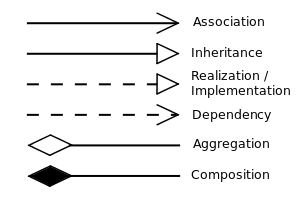
\includegraphics[scale=0.5]{OOPandUML/uml_arrow_cheatsheet}
        \caption{UML logical connectors}
        \label{fig:uml-arrows}
    \end{figure}
    \begin{itemize}
        \item \textbf{Association}\\ 
              a \highlightit{relationship bewteen classes 
              of objects} that allows one object instance to cause another 
              \highlightit{to perform an action on its behalf}.
              \newline
              This relationship is structural and does not represent 
              any behavioural trait.
              \newline
              Code implementation usually requires the requsting object 
              to invoke a method or member function using a 
              \highlightit{reference or a pointer to the controlled 
              object}.
              \newline
              Association can be \highlightit{bidirectional, 
              unidirectional, aggregation and reflexive}.
              \newline
              Objects related via the association are considered to act 
              in a role with respect to the association.
              \newline
              The ends of the association can have all the 
              characteristics of a property: 
              \newline
              \highlightit{multiplicity, name, 
              visibility and a specification} explaining whether the 
              association is ordered and / or unique.
              
        \item \textbf{Dependency}\\ 
              a relationship showing that \highlightit{an element requires 
              other model elements} for their specification or implementation. 
              \newline
              The dashed lines from the dependent/client to 
              the independent/supplier element specifies 
              \highlightit{the direction of a relationship and not of a process}.
              
        \item \textbf{Aggregation}\\
              a variant of \highlightit{has a association relationship 
              and more specific than the latter}. 
              It represents a part-whole or a part-of relationship. 
              As a type of association, an aggregation can be named and 
              have the same adornments an association can.
              \newline
              An aggregation \highlightit{can occur when a class is a 
              collection or a container of other classes}, but 
              \highlightit{the content of the container continues 
              to exist when the container is destroyed}.
              \newline
              In UML notation, the \highlightit{hollow diamond shape is 
              drawn on the containing class end} of the connecting line. 
              \newline
              An example of aggregarion is a Pond which has zero or more 
              Ducks and Duck which has at most one Pond.
              \newline
              \highlightit{A duck can exist separately from a pond}.
              
        \item \textbf{Composition}\\ 
              refers to \highlightit{combining objects within 
              compound objects, ensuring the encapsulation} of each 
              object by \highlightit{using the well-defined interface without 
              exposing the internals}. Differently, data structures do 
              not enforce encapsulation.
              \newline
              Composition can be regarded as a \highlightit{relationship 
              between types}: an object of composite type \highlightit{has} objects 
              of other types
              \newline
              \highlightit{Composition must be distinguished from subtyping}, 
              which is the process of adding detail to a general data type 
              to create a more specific one.
              \newline
              In UML notation, the \highlightit{filled diamond shape is 
              drawn on the containing class end} of the connecting line. An example of 
              composition is a University which has one or more 
              Departments, which belong exactly to one Univerity.
              \newline
              \highlightit{A Department can not exist as a separate entity} 
              detached from a specific University.
    \end{itemize}
    %%% Composition versus Aggregation
    %~ \nparagraph{Composition versus Aggregation}
    %~ \begin{itemize}
        %~ \item Composition relationship
        %~ \item Aggregation relationship
    %~ \end{itemize}
    %%% Class level relationship
    \subsubsection{Class-level relationships}
    \begin{itemize}
        \item \textbf{Generalization/Inheritance}
              \newline
              a relationship between two classes, in which the \highlightit{subclass} is 
              considered to be a specialization from the \highlightit{super type}. 
              \newline
              \highlightit{Any instance of the subtype is also an instance 
              of the superclass}. 
              As an example, \\
              \highlightit{humans are a subclass of simian which is a subclass of mammal}.
              \newline
              Generalization is also known as \highlightbf{inheritance} or a 
              \highlightit{is a} relationship. 
              \newline
              The base class is also known as parent, superclass, 
              base class or base type.
              \newline
              The subtype is also known as child, subclass, 
              derived class, derived type, inheriting class or 
              inheriting type.
        \item \textbf{Realization/Implementation}
              \newline
              a relationship between two model elements, in which
              the \highlightit{client} realizes (implements or executes) the behavior 
              that the \highlightit{supplier} specifies.
    \end{itemize}
    %%% General relationship
    \subsubsection{General relationship}
    \begin{itemize}
        \item \textbf{Dependency}\\
              a weaker form of bond that indicates that one class depends 
              on another because it uses it at some point in time. 
              Sometimes this relationship might be implemented as member 
              function arguments.
        \item \textbf{Multiplicity}\\
              an optional notation which can be 
              useful to add details to the association relationship. At 
              each end of the line, one of the following notation can be 
              used to indicate the range of number of objexts that 
              partecipate in the association from the perspective of the 
              other end.
             \begin{table}[ht]
                 \begin{center}
                     \begin{tabular}{l l}
                         $0$ & No instances\\
                         $0..1$ \quad & No instances, or one instance\\
                         $1$ & Exactly one instance\\
                         $1..1$ & Exactly one instance\\
                         $0..*$ & Zero or more instances\\
                         $*$ & Zero or more instances\\
                         $1..*$ & One or more instances\\
                     \end{tabular}
                 \end{center}
             \end{table}
    \end{itemize}

    \subsubsection{Class and Sequence diagram Cheatsheet}
    Following \highlightit{a summary of the information for class and sequance UML 
    diagrams}
    \begin{figure}[H]
        \centering
        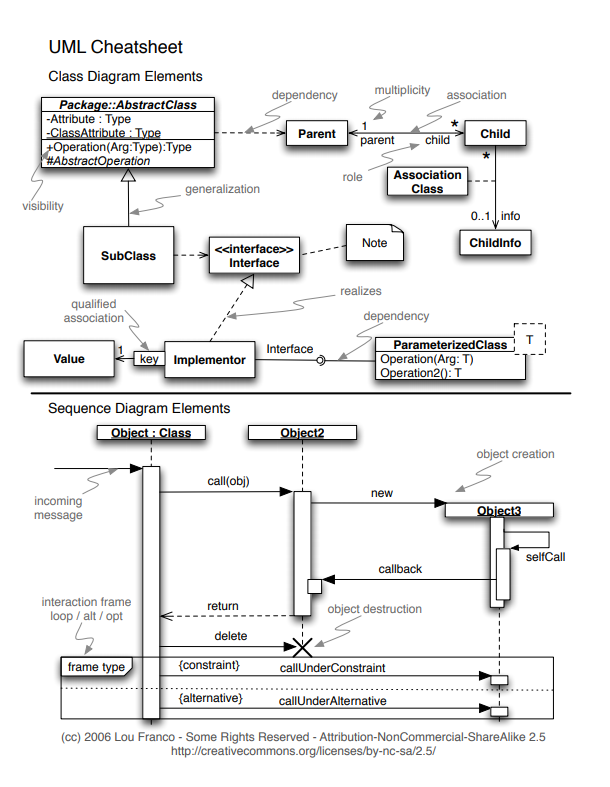
\includegraphics[scale=0.7]{OOPandUML/uml_class_sequence_diag_cheatsheet}
        \caption{Class and Sequence diagrams cheatsheet}
        \label{fig:class-seq-diag-cheatsheet}
    \end{figure}

    \subsection{Sequence Diagram}
    
%%% OOP.
\section{Object Oriented Programming}
    \subsection{Polymorphism}
    In C++ there are different kinds of polymorphism, summarized it 
    the figure~\ref{fig:cpp-poly}
    \begin{figure}[H]
        \centering
        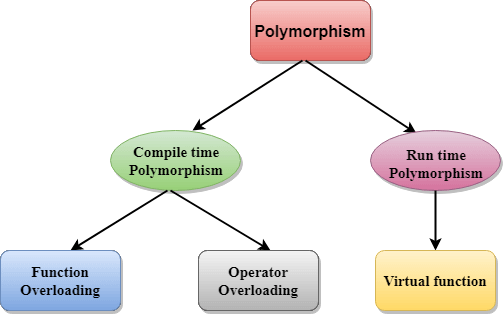
\includegraphics[scale=0.5]{OOPandUML/cpp_polymorphism}
        \caption{Polimorphism in C++}
        \label{fig:cpp-poly}
    \end{figure}
    \subsubsection*{Compile time polymorphism}
    \highlightit{Overloaded functions} are invoked by matching the type 
    and number of arguments at compile time, because the compiler already has all the 
    information needed. This is know by the name of 
    \highlightit{static binding} or \highlightit{early binding}.
    \subsubsection*{Run time polymorphism}

\subsection{Interface vs Abstract class}
\begin{itemize}
    \item Interface can contain only body-less abstract 
    \item Abstract Class
\end{itemize}

\newpage
\printbibsection{subbibintoc}{umlandoop}{UML and OOP Bibliography}
\part{Other Topics}
\chapter{Python}
\label{chap:python}
\vspace{10.5cm}
%~ foo
%~ \newpage{}
\section{PEP}
\section{Built-in Data TYpes}
\subsection{\href{https://docs.python.org/3/library/stdtypes.html\#dict}{dict}}
\subsection{\href{https://docs.python.org/3/library/stdtypes.html\#list}{list}}
\subsection{\href{https://docs.python.org/3/library/stdtypes.html\#set}{set}}
\subsection{\href{https://docs.python.org/3/library/stdtypes.html\#frozenset}{frozenset}}
\subsection{\href{https://docs.python.org/3/library/stdtypes.html\#tuple}{tuple}}
\subsection{\href{https://docs.python.org/3/library/stdtypes.html\#string}{string}}
\subsection{\href{https://docs.python.org/3/library/stdtypes.html\#bytes}{bytes}}
\subsection{\href{https://docs.python.org/3/library/stdtypes.html\#bytearray}{bytearray}}

\newpage
\section{Decorator}
A function decorator is a callable object that takes a function as its 
input parameter
\href{https://www.programiz.com/python-programming/decorator}{decorator} \\
\href{https://www.geeksforgeeks.org/decorators-with-parameters-in-python/}{Decorators with parameters} \\
\href{https://wiki.python.org/moin/PythonDecoratorLibrary}{PythonDecoratorLibrary}
\newpage{}
\section{Special Instance Method}
\href{https://docs.python.org/3/reference/datamodel.html#specialnames}{Special Instance Method}


\section{Providing Multiple Ctors}
\href{https://realpython.com/python-multiple-constructors/}{multiple \texttt{\char`_\char`_init\char`_\char`_}}

\newpage

\newpage
\printbibsection{subbibintoc}{python}{Python Bibliography}
\chapter{Software Testing}
\label{chap:testing}
\vspace{10.5cm}
\section{Seven Tesing Principles}
\section{SDLC vs. STLC}
\section{Unit Testing}

\section{Integration Test and Regression Test}
\subsection{Integration Test}
Integration testing \highlightit{checks the communication and data flow between 
two modules}
\newline 
\highlightit{of the same system after integrating them}. \\
A software consists of \highlightit{several small modules} that carry certain features 
and come together to build the system. 
Sometimes even when these modules pass the quality test independently, 
they \highlightit{might encounter data flow issues upon integration}. 
\newline
Integration testing verifies the \highlightit{compatibility between these individual 
parts} and ensures they work in unison \highlightit{without any issues after integration}. 
It can be a black-box testing or white-box testing technique.
\newline
\highlightit{An example} of integration testing would be checking the logical connection 
between the ‘Proceed to Payment’ page and the payment gateway for an 
e-commerce application.

\subsection{Regression Test}
Regression testing \highlightit{re-checks 
software or an application after new changes are introduced}. 
This testing process runs \highlightit{functional and non-functional checks on the 
existing features}
\newline
\highlightit{of the software to ensure that no issues arise due 
to new code changes}.
\newline
The goal of regression testing is \highlightit{to identify 
any defects in the present system that may}
\newline
\highlightit{occur due to updates/changes}. 
Regression testing can either be white box testing or black box testing.
\newline
You can \highlightit{re-use the test cases} in regression testing to verify the existing 
functionalities. This includes running the same test cases and scripts 
to get the same output that validates the present features.
\newline
\highlightit{An example} of regression testing is checking the Camera, Phone, and other 
applications in your mobile after a system update. Smartphones often receive 
regular system updates that can hamper the ongoing functions of the phone. 
Regression testing would assess if any OS or parts upgrade impacted your phone.


\subsection{terms from the youtube video}
\begin{itemize}
    \item decision coverage
    \item predicate coverage
    \item all path coverage
    \item boundary coverage
    \item black box testing
    \item white box testing
\end{itemize}

\newpage
\printbibsection{subbibintoc}{testing}{Testing Bibliography}
\chapter{AI}
\label{chap:ai}
\vspace{10.5cm}


\newpage
\printbibsection{subbibintoc}{ai}{AI Bibliography}
\part{Reference}
\setboolean{@twoside}{true} 
\clearpage
\pagestyle{dictionarystyle}

\chapter{Dictionary}
\label{chap:dictionary}

\subsection{A}

\begin{multicols*}{2}

    \dictentry{ABA}{CAS failure mode where a location returns to an old value 
    after intervening updates, so compare-and-swap succeeds incorrectly; 
    mitigated with tags or safe reclamation (Chapter~\ref{chap:memorymodel}).}

    \dictentry{ADL}{Argument Dependent Lookup}
        
    \dictentry{ADT}{Abstract Data Type}

    \dictentry{AF\_XDP}{Address Family XDP: Linux socket type for high-performance 
    packet I/O with zero-copy options; a kernel-bypass-adjacent path 
    (Chapter~\ref{chap:kernelbypass}).}

    \dictentry{Affinity}{binding a thread (or IRQ) to a CPU set so it does not 
    migrate; pairs with \texttt{isolcpus} and NUMA placement 
    (Chapter~\ref{chap:linuxprocesses}).}

    \dictentry{Allocate}{to assign, allot, distribute, or set apart for 
    a particular purpose}

    \dictentry{Allocator (C++)}{type that satisfies the Allocator requirements and 
    supplies \texttt{allocate}/\texttt{deallocate} for containers; PMR variants use 
    a runtime \texttt{memory\char`_resource} (Section~\ref{subsec:custom-allocators}).}

    \dictentry{Amortized}{cost of an operation averaged over a long sequence 
    (e.g.\ \texttt{vector::push\char`_back}); one step may be expensive, the 
    sequence is cheap (Section~\ref{subsec:amortized-vs-average}).}

    \dictentry{Arena}{preallocated memory region from which many objects are 
    carved; avoids hot-path \texttt{malloc} (Chapter~\ref{chap:memmag}).}

    \dictentry{Atomic}{Objects of atomic types are the only C++ objects 
    that are free from data races; that is, if one thread writes to an 
    atomic object while another thread reads from it, the behavior is 
    well-defined. In addition, accesses to atomic objects may establish 
    inter-thread synchronization and order non-atomic memory accesses 
    as specified by \textbf{\texttt{std::memory\char`_order}}.}
    
\end{multicols*}

\subsection{B}
\begin{multicols*}{2}

    \dictentry{BBO}{Best Bid and Offer: top-of-book prices (and often sizes); 
    the first level of the order book (Chapter~\ref{chap:algorithms}).}

    \dictentry{Big O}{asymptotic upper-bound notation for growth of time or 
    space with input size (Chapter~\ref{chap:algorithms}).}

    \dictentry{Black--Scholes}{classic continuous-time option pricing model; 
    basis for implied volatility (Chapter~\ref{chap:quantbasics}).}

    \dictentry{branch}{a mean for teams to develop features giving them 
    a separate workspace for their code. The branch to create are part 
    of the branching strategy, which could be different depending on 
    the specific svn used.}

    \dictentry{Busy polling}{spinning on I/O or a queue instead of sleeping 
    (e.g.\ \texttt{SO\char`_BUSY\char`_POLL}, epoll timeout 0); lower latency, 
    higher CPU use (Chapter~\ref{chap:lowlatency}).}

\end{multicols*}

\subsection{C}
\begin{multicols*}{2}

    \dictentry{Cache coherence}{protocol that keeps multiple CPU caches 
    consistent for shared lines (e.g.\ MESI); basis of false sharing 
    (Chapter~\ref{chap:cacheperformance}).}

    \dictentry{Cache line}{granularity of cache transfers and coherence 
    (often 64\,B); pad hot fields to avoid false sharing 
    (Chapter~\ref{chap:cacheperformance}).}

    \dictentry{CAS}{Compare-And-Swap: atomic read-modify-write that updates a 
    location only if it still holds an expected value 
    (\texttt{compare\char`_exchange\char`_*} in C++); basis of many lock-free 
    structures (Chapter~\ref{chap:memorymodel}).}

    \dictentry{CFS}{Completely Fair Scheduler: default Linux policy 
    (\texttt{SCHED\char`_OTHER}); migrates work across CPUs unless isolated 
    (Chapter~\ref{chap:linuxprocesses}).}

    \dictentry{Context switch}{saving/restoring thread or process CPU state 
    when the scheduler runs another task; costs $\mu$s and adds jitter 
    (Chapter~\ref{chap:linuxprocesses}).}

    \dictentry{constexpr}{a C++ specifier which declares that it is 
    possible to evaluate the value of the function or variable 
    at compile time.}

    \dictentry{CPU affinity}{see Affinity.}

\end{multicols*}

\subsection{D}

\begin{multicols*}{2}

    \dictentry{data race}{undefined behavior in C++ when two threads access the 
    same memory location, at least one access is a write, and the accesses are 
    not ordered by the memory model (Chapter~\ref{chap:memorymodel}).}

    \dictentry{deadlock}{any situation in which no member of some group 
    of entities can proceed because each waits for another member, 
    including itself, to take action, such as sending a message or, 
    more commonly, releasing a lock}

    \dictentry{Dependency injection}{design technique where a component receives 
    its dependencies from the outside (constructor/setter/framework) instead of 
    creating them itself; improves testability and decoupling.}

    \dictentry{DPDK}{Data Plane Development Kit: user-space packet processing 
    with poll-mode drivers; a common kernel-bypass stack 
    (Chapter~\ref{chap:kernelbypass}).}

    \dictentry{DSU}{Disjoint Set Union (Union--Find): nearly $O(1)$ amortized 
    connectivity queries (Section~\ref{subsec:pat-uf}).}

    \dictentry{duck typing}{a concept related to \textit{dynamic typing}, 
    where the type or the class of an object is less important than the 
    methods it defines}
    
    \dictentry{double dispatch}{choosing a method from the runtime types of 
    \emph{two} objects (e.g.\ Visitor): a single virtual call is not enough; 
    typically one virtual on the element then a virtual on the visitor.}
    
    \dictentry{dynamic binding}{selecting which function body runs at run time 
    (typically via \texttt{virtual} functions); opposed to static / early binding 
    (Section~\ref{sec:cpp-polymorphism}).}

\end{multicols*}

\subsection{E}
\begin{multicols*}{2}

    \dictentry{encapsulation}{preventing unauthorized access to some piece of information or functionality}

    \dictentry{Epoch reclaim}{safe memory reclamation for lock-free structures 
    by retiring nodes only after all threads leave a shared epoch 
    (Chapter~\ref{chap:memorymodel}).}

    \dictentry{EPOLLET}{edge-triggered \texttt{epoll}: notify on state change; 
    must drain until \texttt{EAGAIN} (Chapter~\ref{chap:eventdrivenio}).}

    \dictentry{epoll}{Linux scalable I/O event notification 
    (\texttt{epoll\char`_create}/\texttt{ctl}/\texttt{wait}); preferred over 
    \texttt{select}/\texttt{poll} for many file descriptors 
    (Chapter~\ref{chap:eventdrivenio}).}

\end{multicols*}

\subsection{F}
\begin{multicols*}{2}

    \dictentry{False sharing}{performance pathology where threads update different 
    variables on the same cache line, causing coherence ping-pong 
    (Chapter~\ref{chap:cacheperformance}).}

    \dictentry{First-touch}{NUMA page placement: a page is usually bound to the 
    node of the CPU that first writes it; pin threads before warm-up 
    (Chapter~\ref{chap:numa}).}

    \dictentry{FIX}{Financial Information eXchange: tag-value messaging standard 
    for many order/broker links; not usually the colocated matching-engine hot path 
    (Section~\ref{sec:market-wire-protocols}).}

    \dictentry{FOK}{Fill-or-Kill: execute the full quantity immediately or cancel 
    (Chapter~\ref{chap:quantbasics}).}

\end{multicols*}

\subsection{G}
\begin{multicols*}{2}

    \dictentry{Greeks}{option risk sensitivities (e.g.\ delta, gamma, theta, vega) 
    (Chapter~\ref{chap:quantbasics}).}

    \dictentry{GTC}{Good-Till-Cancel: order remains until filled or cancelled 
    (Chapter~\ref{chap:quantbasics}).}

\end{multicols*}

\subsection{H}

\begin{multicols*}{2}

    \dictentry{Happens-before}{memory-model relation that defines when one 
    operation's side effects are visible to another; established by 
    mutexes, atomics, etc.\ (Chapter~\ref{chap:memorymodel}).}

    \dictentry{Hazard pointers}{safe reclamation scheme: readers publish 
    pointers they may dereference; reclaimers skip those nodes 
    (Chapter~\ref{chap:memorymodel}).}

    \dictentry{Heap}{a large pool of memory used to satisfy memory 
    request by allocating part.}

    \dictentry{Huge pages}{large page sizes (e.g.\ 2\,MiB) that reduce TLB 
    pressure for big working sets (Chapter~\ref{chap:cacheperformance}).}

\end{multicols*}

\subsection{I}

\begin{multicols*}{2}

    \dictentry{Idiom}{a group of code fragments sharing an equivalent 
    semantic role (meaning), which recurs frequently across software 
    projects often expressing a special feature in one or more 
    programming languages or libraries.}

    \dictentry{Implied vol}{market price of an option expressed as the 
    Black--Scholes volatility that matches it (Chapter~\ref{chap:quantbasics}).}

    \dictentry{Interrupt coalescing}{NIC/driver (or OS) batches several packet 
    arrivals into fewer hard IRQs to raise throughput and cut interrupt rate. 
    That saves CPU but adds latency and jitter --- usually the wrong trade for 
    tick-to-trade paths (Chapter~\ref{chap:lowlatency}).}

    \dictentry{IOC}{Immediate-or-Cancel: take what is available now, cancel 
    the rest (Chapter~\ref{chap:quantbasics}).}

    \dictentry{I/O mux}{waiting on many file descriptors for readiness 
    (\texttt{select}/\texttt{poll}/\texttt{epoll}) 
    (Chapter~\ref{chap:eventdrivenio}).}

    \dictentry{irqaffinity}{kernel boot parameter setting the default CPU mask 
    for IRQs; keep defaults on housekeeping cores so isolated CPUs stay quiet 
    (Section~\ref{subsec:irq-affinity}).}

    \dictentry{irqbalance}{userspace daemon that reshuffles IRQ-to-CPU affinity 
    at runtime; disable or constrain on latency boxes or it undoes manual 
    \texttt{smp\char`_affinity} (Section~\ref{subsec:irq-affinity}).}

    \dictentry{isolcpus}{kernel boot parameter that removes CPUs from the general 
    scheduler balance set (scheduling exclusion); used with pinning for dedicated 
    HFT cores (Section~\ref{subsec:isolcpus}).}

    \dictentry{ITCH}{family of binary multicast market-data protocols 
    (order-book incremental updates) (Section~\ref{sec:market-wire-protocols}).}

    \dictentry{Iter. invalid.}{when a container operation makes iterators or 
    references unusable (e.g.\ \texttt{vector} reallocation) 
    (Section~\ref{sec:iterator-invalidation}).}

\end{multicols*}

\subsection{J}
\begin{multicols*}{2}

    \dictentry{Jitter}{variability of latency (not just the mean); isolation 
    and allocation-free paths target lower jitter (Chapter~\ref{chap:lowlatency}).}

\end{multicols*}

\subsection{K}
\begin{multicols*}{2}

    \dictentry{Kernel bypass}{moving packet path out of the kernel networking 
    stack (DPDK, OpenOnload, AF\_XDP, \ldots) to cut syscall/copy overhead 
    (Chapter~\ref{chap:kernelbypass}).}

\end{multicols*}

\subsection{L}
\begin{multicols*}{2}

    \dictentry{Locality}{spatial: nearby addresses used together; temporal: 
    same addresses reused soon; drives cache-friendly layout 
    (Chapter~\ref{chap:cacheperformance}).}

    \dictentry{Lock convoy}{many threads queueing on one mutex so throughput 
    collapses under contention (Chapter~\ref{chap:memorymodel}).}

    \dictentry{Lock-free}{algorithm that guarantees system-wide progress even if 
    some threads are delayed; typically built with atomics/CAS, not wait-free 
    for every thread (Chapter~\ref{chap:memorymodel}).}

    \dictentry{L1 (MD)}{market-data top-of-book (BBO) feed depth 
    (Chapter~\ref{chap:quantbasics}).}

    \dictentry{L2 (MD)}{market-data aggregated depth by price level 
    (Chapter~\ref{chap:quantbasics}).}

    \dictentry{L3 (MD)}{market-data full order-by-order / order-id book 
    (Chapter~\ref{chap:quantbasics}).}

\end{multicols*}

\subsection{M}
\begin{multicols*}{2}

    \dictentry{Matching engine}{venue component that matches orders and 
    publishes trades / book updates (Chapter~\ref{chap:quantbasics}).}

    \dictentry{Memory order}{C++ atomic ordering: \texttt{relaxed}, 
    \texttt{acquire}, \texttt{release}, \texttt{acq\char`_rel}, 
    \texttt{seq\char`_cst}; controls visibility and reordering 
    (Chapter~\ref{chap:memorymodel}).}

    \dictentry{MESI}{Modified / Exclusive / Shared / Invalid cache-coherence 
    protocol states (Chapter~\ref{chap:cacheperformance}).}

    \dictentry{method chaining}{API style where setters / builders return 
    \texttt{*this} (or a proxy) so calls can be written 
    \texttt{obj.setA(1).setB(2)}; common in the Named Parameter idiom.}

    \dictentry{mmap}{POSIX call that maps files or anonymous pages into a process 
    address space; basis for memory-mapped I/O and some shared memory 
    (Chapter~\ref{chap:memorymapping}).}

    \dictentry{mock}{test double that stands in for a dependency and records / 
    asserts how it was used (calls, arguments); contrasts with a stub, which 
    mostly returns canned data.}

    \dictentry{most vexing parsing}{C++ grammar ambiguity where a declaration 
    looks like an object definition but is parsed as a function declaration 
    (e.g.\ \texttt{TimeKeeper t(Timer());}); fix with extra parentheses or braces.}

    \dictentry{MPMC}{Multi-Producer Multi-Consumer queue; heavier than SPSC 
    (e.g.\ Michael--Scott) (Chapter~\ref{chap:memorymodel}).}

\end{multicols*}

\subsection{N}
\begin{multicols*}{2}

    \dictentry{Nagle}{TCP algorithm that coalesces small sends; disable with 
    \texttt{TCP\char`_NODELAY} for latency paths (Chapter~\ref{chap:linuxnetworking}).}

    \dictentry{NAPI}{Linux networking softirq path that polls the NIC after 
    an interrupt; can still preempt user threads 
    (Chapter~\ref{chap:kernelbypass}).}

    \dictentry{nohz\_full}{kernel boot option enabling adaptive-ticks / tickless 
    behaviour on listed CPUs (fewer scheduler timer interrupts when a single 
    task runs); often paired with \texttt{isolcpus} / \texttt{rcu\char`_nocbs} 
    (Section~\ref{subsec:nohz-full}).}

    \dictentry{NUMA}{Non-Uniform Memory Access: multi-socket systems where local 
    DRAM is faster than remote; place threads, memory, and NICs carefully 
    (Chapter~\ref{chap:numa}).}

\end{multicols*}

\subsection{O}

\begin{multicols*}{2}

    \dictentry{Object pool}{reuse preconstructed objects instead of 
    allocating on the hot path (Chapter~\ref{chap:memmag}).}

    \dictentry{OpenOnload}{Solarflare/Xilinx kernel-bypass stack that accelerates 
    sockets in user space (Chapter~\ref{chap:kernelbypass}).}

    \dictentry{object}{region of storage with associated semantics}

    \dictentry{Order book}{local structure of resting bids and asks by price 
    (and often order id); updated from market data (Chapter~\ref{chap:algorithms}).}

    \dictentry{Overloading}{a compile time polymorphism achieved 
    specifying more than one function with the same name but different 
    signature in the same scope.}
    
    \dictentry{Overridding}{the act of redefining a method of a base 
    class in a derived class, using the same name, return type and 
    parameters.}

\end{multicols*}

\subsection{P}

\begin{multicols*}{2}

    \dictentry{Page fault}{CPU trap when a virtual page is not mapped or not 
    present; major faults hit disk/IO and blow hot-path latency 
    (Chapter~\ref{chap:linuxprocesses}).}

    \dictentry{Parameterized type}
              {another definition for \highlight{class templates}.}

    \dictentry{perf}{Linux profiling tool (\texttt{perf record}/\texttt{stat}) 
    for cycles, cache misses, false sharing hunts 
    (Chapter~\ref{chap:cacheperformance}).}

    \dictentry{Pinning}{see Affinity.}

    \dictentry{PMD}{Poll-Mode Driver: NIC driver that busy-polls rings 
    (DPDK-style) instead of interrupt-driven RX (Chapter~\ref{chap:kernelbypass}).}

    \dictentry{PMR}{Polymorphic Memory Resource (\texttt{std::pmr}): runtime-selected 
    \texttt{memory\char`_resource} behind containers 
    (Section~\ref{subsec:custom-allocators}).}

    \dictentry{poll}{POSIX I/O multiplexer; improves on \texttt{select} but still 
    scales worse than \texttt{epoll} for large FD sets 
    (Chapter~\ref{chap:eventdrivenio}).}

    \dictentry{Polymorphysm}
              {ability of different objects to be accessed by a common 
              interface.}
                      
\end{multicols*}

%~ \subsection{Q}
%~ \begin{multicols*}{2}\end{multicols*}

\subsection{R}

\begin{multicols*}{2}
    
    \dictentry{Race Condition}{undesirable situation which occurs when 
    two instructions from different threads access the same memory 
    location, at least one of these accesses is a write and there is no 
    synchronization that is mandating any particular order among these 
    accesses.}
    
    \dictentry{RAII}{acronym for Resource Acquisition Is Initialization.}
    
    \dictentry{RBV optimization}{see~\cite{isocpp-rbv-optimization}.}

    \dictentry{RCU}{Read-Copy-Update: Linux synchronization for read-heavy shared 
    data; writers defer freeing old versions via callbacks. Those callbacks can 
    jitter isolated CPUs unless offloaded with \texttt{rcu\char`_nocbs} 
    (Section~\ref{subsec:rcu-nocbs}).}

    \dictentry{rcu\_nocbs}{kernel boot option that offloads RCU callback processing 
    from listed CPUs onto housekeeping cores (Section~\ref{subsec:rcu-nocbs}).}

    \dictentry{Reactor}{event-loop style: demultiplex I/O readiness then 
    dispatch handlers (typical \texttt{epoll} server) 
    (Chapter~\ref{chap:eventdrivenio}).}

    \dictentry{RTTI}{acronym for Run-Time Type Information: language mechanism 
    that exposes dynamic type of polymorphic objects (e.g.\ \texttt{typeid}, 
    \texttt{dynamic\char`_cast}). Requires a polymorphic type (usually a virtual 
    function); typically implemented via type info reachable from the vtable. 
    Can be disabled with compiler flags (\texttt{-fno-rtti}) to save space/cost.}

    \dictentry{RVO}{acronym for Return Value Optimization.}

\end{multicols*}

\subsection{S}
\begin{multicols*}{2}

    \dictentry{SBE}{Simple Binary Encoding: compact, schema-driven binary 
    messages for market data / OE (Section~\ref{sec:market-wire-protocols}).}

    \dictentry{SCHED\_FIFO}{Linux real-time FIFO scheduling policy; use carefully 
    on dedicated cores (Chapter~\ref{chap:linuxprocesses}).}

    \dictentry{SCHED\_RR}{Linux real-time round-robin scheduling policy 
    (Chapter~\ref{chap:linuxprocesses}).}

    \dictentry{select}{classic POSIX I/O multiplexer with an FD-count limit and 
    $O(n)$ scans; prefer \texttt{poll}/\texttt{epoll} for scale 
    (Chapter~\ref{chap:eventdrivenio}).}

    \dictentry{Seq. consistency}{strongest C++ atomic default 
    (\texttt{memory\char`_order\char`_seq\char`_cst}): a single total order of 
    all seq\_cst ops (Chapter~\ref{chap:memorymodel}).}

    \dictentry{smp\_affinity}{per-IRQ CPU mask under 
    \texttt{/proc/irq/<n>/smp\char`_affinity} (or 
    \texttt{smp\char`_affinity\char`_list}); steer hard IRQs (e.g.\ NIC queues) 
    onto housekeeping cores (Section~\ref{subsec:irq-affinity}).}

    \dictentry{softirq}{deferred kernel interrupt work (e.g.\ networking) that 
    can run on a CPU and add jitter (Chapter~\ref{chap:kernelbypass}).}

    \dictentry{Spinlock}{busy-wait lock for very short critical sections; 
    burns CPU while waiting (Chapter~\ref{chap:memorymodel}).}

    \dictentry{Spread}{difference between best ask and best bid 
    (Chapter~\ref{chap:quantbasics}).}
    
    \dictentry{static typing}{types are checked at compile time; variables and 
    expressions have types known to the compiler (as in C++), opposed to 
    dynamic typing where much checking happens at run time.}
    
    \dictentry{SFINAE}{acronym for \textbf{Substitution} \textbf{Failure} 
    \textbf{Is} \textbf{Not} \textbf{An} \textbf{Error}, a technique 
    used in template programming which discards the specialization from 
    the overloaded set avoiding a compile error, when substituting the 
    explicitly specified or deduced type for the template parameter fails.}

    \dictentry{SPSC}{Single-Producer Single-Consumer queue (often a ring buffer): 
    lock-free handoff between exactly two threads 
    (Section~\ref{sec:spsc-ring-buffer}).}
    
    \dictentry{Stack}{LIFO-ordered contiguous region of temporary memory 
    whose size is known to the compiler, which manages to allocate and 
    deallocate blocks of memory for the stack variables like functions' 
    local data. . If a region of memory lies on the thread's stack, 
    that memory is said to have been allocated on the stack, i.e. 
    stack-based memory allocation (SBMA).}
    
    \dictentry{Stub}{test double that provides canned answers to calls; lighter 
    than a mock (which also verifies interaction). In broader software slang, 
    also an unfinished placeholder implementation.}

    \dictentry{Syscall}{trap from user space into the kernel (e.g.\ 
    \texttt{recv}, \texttt{epoll\char`_wait}); mode switch cost motivates 
    bypass (Chapter~\ref{chap:kernelbypass}).}

\end{multicols*}


\newpage{}
\subsection{T}
\begin{multicols*}{2}

    \dictentry{Tail latency}{high percentiles of latency (p99 / p999), not the 
    mean; HFT cares about tails and jitter (Chapter~\ref{chap:lowlatency}).}

    \dictentry{TCP\_NODELAY}{socket option that disables Nagle coalescing for 
    lower send latency (Chapter~\ref{chap:linuxnetworking}).}

    \dictentry{template function}
              {instantiation of a function template}

    \dictentry{Test-driven Development}
              {\href{https://en.wikipedia.org/wiki/Test-driven_development}{wikipedia}}

    \dictentry{tick-to-trade}{end-to-end latency from receiving a market event 
    to sending an order (Chapter~\ref{chap:lowlatency}).}

    \dictentry{TLB}{Translation Lookaside Buffer: CPU cache of 
    virtual$\rightarrow$physical address translations 
    (Chapter~\ref{chap:cacheperformance}).}

    \dictentry{Type erasure}{hiding a concrete type behind a uniform interface 
    (virtuals, \texttt{std::function}/\texttt{any}, or a custom eraser); related 
    but not identical to opaque \texttt{void*} payloads 
    (Section~\ref{subsec:type-erasure}).}

\end{multicols*}

\subsection{U}
\begin{multicols*}{2}

    \dictentry{Union--Find}{see DSU.}

\end{multicols*}

\subsection{V}
\begin{multicols*}{2}
    
    \dictentry{virtual member function}{a mean to allow derived classes 
    to replace the implementation provided by the base class. The 
    compiler makes sure to call the correct replacement when 
    the object is of the derived class and also when the object is 
    accessed through a pointer to the base rather than to the derived 
    class.}
    
\end{multicols*}

\subsection{W}
\begin{multicols*}{2}

    \dictentry{Wait-free}{stronger than lock-free: every thread completes 
    its operation in a bounded number of its own steps 
    (Chapter~\ref{chap:memorymodel}).}

\end{multicols*}

\subsection{X}
\begin{multicols*}{2}

    \dictentry{XDP}{eXpress Data Path: early in-kernel packet hook; 
    AF\_XDP exposes XDP rings to user space (Chapter~\ref{chap:kernelbypass}).}

\end{multicols*}

%~ \subsection{Y}
%~ \begin{multicols*}{2}\end{multicols*}

\subsection{Z}
\begin{multicols*}{2}

    \dictentry{Zero-copy}{I/O path that avoids copying packet/payload bytes 
    between kernel and user buffers (Chapter~\ref{chap:kernelbypass}).}

\end{multicols*}



\setboolean{@twoside}{false} 
\pagestyle{basicstyle}

\newpage
\printbibsection{subbibintoc}{dictionary}{Dictionary Bibliography}
\newpage
\pagestyle{basicstyle}
\chapter{References}
\label{chap:references}
\printbibliography[heading=none]



\end{document}
